\documentclass[twoside,11pt]{article}

% Any additional packages needed should be included after jmlr2e.
% Note that jmlr2e.sty includes epsfig, amssymb, natbib and graphicx,
% and defines many common macros, such as 'proof' and 'example'.
%
% It also sets the bibliographystyle to plainnat; for more information on
% natbib citation styles, see the natbib documentation, a copy of which
% is archived at http://www.jmlr.org/format/natbib.pdf

\usepackage{jmlr2e}
 \usepackage{lastpage}
\usepackage{smile_jmlr}
 \usepackage{mathtools}

 
 \newtheorem{assumption}[theorem]{Assumption}
            
% Definitions of handy macros can go here

  \newcommand{\defeq}{\vcentcolon=}
 
\newcommand*{\BR}{\mathbb{R}}
\newcommand*{\BB}{\mathbb{B}}
\newcommand*{\hbgamma} {\hat{\bgamma}}
\newcommand*{\tbdelta}{\tilde \bdelta}
\newcommand*{\hbdelta}{\hat\bdelta}


\newcommand*{\Sc}{\cS^{\perp}}
\newcommand*{\Ac}{\cA^{\perp}}
\newcommand*{\supp}{\mathrm{supp}}
\newcommand*{\tx}{\tilde{\bx}}
\newcommand*{\tX}{\tilde{\bx}}
\newcommand*{\hbbeta}{\hat{\bbeta}}
\newcommand*{\hbbetanull}{0,\hbbeta_{\setminus _{st}}}
\newcommand*{\tbbeta}{\tilde{\bbeta}}
\newcommand*{\bbetas}{\bbeta^*}
\newcommand*{\hdbeta}{\hat{\bbeta}^d}
\newcommand*{\beq}{\begin{equation}}
\newcommand*{\eeq}{\end{equation}}
\newcommand*{\bbDelta}{\hat{\bDelta}}
\newcommand*{\tbDelta}{\tilde{\bDelta}}
\newcommand*{\gradstar} {\nabla L (\bbeta^*)}
\newcommand*{\grad} {\nabla L(\bbeta)}
\newcommand*{\hgrad} {\nabla L (\hbbeta)}
\newcommand*{\tgrad}{\nabla L(\tbbeta)}
\newcommand*{\hessstar}{\nabla^2  \ell(\bbeta^*)}
\newcommand*{\hess}{\nabla^2  L(\bbeta)}
\newcommand*{\hhess}{\nabla^2  L(\hbbeta)}
\newcommand*{\thess}{\nabla^2  L(\tbbeta)}

\newcommand*{\gradstars} {\nabla L_j(\bbeta^*)}
\newcommand*{\grads} {\nabla L_j(\bbeta)}
\newcommand*{\hgrads} {\nabla L_j(\hbbeta)}
\newcommand*{\tgrads}{\nabla L_j(\tbbeta)}
\newcommand*{\hessstars}{\nabla^2  L_j(\bbeta^*)}
\newcommand*{\hesss}{\nabla^2  L_j(\bbeta)}
\newcommand*{\hhesss}{\nabla^2  L_j(\hbbeta)}
\newcommand*{\thesss}{\nabla^2  L_j(\tbbeta)}

\newcommand*{\gradstarst} {\nabla L_{jk}\bigl(\bbeta_{j\vee k}^*\bigr)}
\newcommand*{\gradst} {\nabla L_{jk}\bigl(\bbeta_{j \vee k}\bigr)}
\newcommand*{\hgradst} {\nabla L_{jk}\bigl(\hbbeta_{j \vee k}\bigr)}
\newcommand*{\tgradst}{\nabla L_{jk}\bigl(\tbbeta_{j \vee k}\bigr)}
\newcommand*{\hessstarst}{\nabla^2  L_{jk}\bigl(\bbeta_{j \vee k}^*\bigr)}
\newcommand*{\hessst}{\nabla^2  L_{jk}\bigl(\bbeta_{j \vee k}\bigr)}
\newcommand*{\hhessst}{\nabla^2  L_{jk}\bigl(\hbbeta_{j \vee k}\bigr)}
\newcommand*{\thessst}{\nabla^2  L_{jk}\bigl(\tbbeta_{j \vee k}\bigr)}

\newcommand*{\gradstarstt} {\nabla \ell_{st}\bigl(\bbeta^*_{\sbb \cup \tb}\bigr)}
\newcommand*{\gradstt} {\nabla \ell_{st}(\bbeta_{\sbb \cup \tb})}
\newcommand*{\hgradstt} {\nabla \ell_{st}(\hbbeta_{\sbb \cup \tb})}
\newcommand*{\tgradstt}{\nabla \ell_{st}(\tbbeta_{\sbb \cup \tb})}
\newcommand*{\hessstarstt}{\nabla^2  \ell_{st}(\bbeta^*_{\sbb \cup \tb})}
\newcommand*{\hessstt}{\nabla^2  \ell_{st}(\bbeta_{\sbb \cup \tb})}
\newcommand*{\hhessstt}{\nabla^2  \ell_{st}(\hbbeta_{\sbb \cup \tb})}
\newcommand*{\thessstt}{\nabla^2  \ell_{st}(\tbbeta_{\sbb \cup \tb})}

\newcommand*{\gradstarss} {\nabla {L_j}(\bbeta^*_{j})}
\newcommand*{\gradss} {\nabla{L_j}(\bbeta_{j})}
\newcommand*{\hgradss} {\nabla {L_j}(\hbbeta_{j})}
\newcommand*{\tgradss}{\nabla {L_j}(\tbbeta_{j})}
\newcommand*{\hessstarss}{\nabla^2 {L_j}(\bbeta^*_{j})}
\newcommand*{\hessss}{\nabla^2  {L_j}(\bbeta_{j})}
\newcommand*{\hhessss}{\nabla^2 {L_j}(\hbbeta_{j})}
\newcommand*{\thessss}{\nabla^2{L_j}(\tbbeta_{j})}

\newcommand*{\gradstarsu} {\nabla {L_j}(\ub)}
\newcommand*{\gradsu} {\nabla{L_j}(\ub)}
\newcommand*{\hgradsu} {\nabla{L_j}(\ub)}
\newcommand*{\tgradsu}{\nabla{L_j}(\ub)}
\newcommand*{\hessstarsu}{\nabla^2 {L_j}(\ub)}
\newcommand*{\hesssu}{\nabla^2 {L_j}(\ub)}
\newcommand*{\hhesssu}{\nabla^2  {L_j}(\ub)}
\newcommand*{\thesssu}{\nabla^2 {L_j}(\ub)}

\newcommand*{\sbbeta}{\bbeta_{j}}
\newcommand*{\hbbetas}{\hat{\bbeta}_{j}}
\newcommand*{\tbbetas}{\tilde{\bbeta}_{j}}
\newcommand*{\bbetass}{\bbeta^*_{j}}


\makeatletter
\newcommand{\rmnum}[1]{\romannumeral #1}
\newcommand{\Rmnum}[1]{\expandafter\@slowromancap\romannumeral #1@}
\makeatother

\def\##1\#{\begin{align}#1\end{align}}
\def\$#1\${\begin{align*}#1\end{align*}}


\newcommand*{\hOmega}{\hat{\bOmega}}
\newcommand*{\hTheta}{\hat{\bTheta}}
\newcommand*{\hSigma}{\hat{\bSigma}}
\newcommand*{\tSigma}{\tilde{\bSigma}}
\newcommand*{\homega}{\hat{\bomega}}
\newcommand*{\hvartheta}{\hat \bvartheta}
\newcommand*{\sW}{\Wb^*}
\newcommand*{\hW}{\hat{\Wb}}
\newcommand*{\hw}{\hat{\wb}}
\newcommand*{\sw}{\wb^*}
\newcommand*{\la}{\langle}
\newcommand*{\ra}{\rangle}
\newcommand*{\limn}{\lim \limits_{n\rightarrow \infty} }

% Heading arguments are {volume}{year}{pages}{date submitted}{date published}{paper id}{author-full-names}

\jmlrheading{1}{2000}{1-48}{4/00}{10/00}{meila00a}{Marina Meil\u{a} and Michael I. Jordan}

% Short headings should be running head and authors last names


\jmlrheading{19}{2018}{1-\pageref{LastPage}}{9/15; Revised
10/18}{10/18}{15-493}{Zhuoran Yang, Yang Ning, Han Liu }
\ShortHeadings{On Semiparametric Exponential Family Graphical Models}{Yang, Ning, and Liu}



 
\firstpageno{1}

\begin{document}

\title{On Semiparametric Exponential Family Graphical Models}

\author{\name Zhuoran Yang \email zy6@princeton.edu \\
       \addr Department of Operations Research and Financial Engineering\\
       Princeton University\\
       Princeton, NJ 08544, USA
       \AND
       \name Yang Ning \email yn265@cornell.edu \\
       \addr Department of Statistical Science\\
       Cornell University\\
       Ithaca,  NY 14853, USA
       \AND
       \name Han Liu \email hanliu@northwestern.edu\\
       \addr Department of Electrical Engineering and Computer Science\\
       Northwestern University\\
       Evanston, IL 60208, USA}

\editor{David Blei}

\maketitle

\begin{abstract}%   <- trailing '%' for backward compatibility of .sty file
We propose a new class of semiparametric exponential family graphical models for the analysis of high dimensional mixed data. Different from the existing mixed graphical models, we allow the nodewise conditional distributions to be semiparametric generalized linear models with unspecified base measure functions. Thus, one advantage of our method is that it is unnecessary to specify the type of each node and the method is more convenient to apply in practice. Under the proposed model, we consider both problems of parameter estimation and hypothesis testing in high dimensions. In particular, we propose a symmetric pairwise score test for the presence of a single edge in the graph. Compared to the existing methods for hypothesis tests, our approach takes into account of the symmetry of the parameters, such that the inferential results are invariant with respect to the different parametrizations of the same edge. 
Thorough numerical simulations and a real data example are provided to back up our theoretical results. \end{abstract}

\begin{keywords}
  Graphical Models, Exponential Family, High Dimensional Inference
\end{keywords}
 
 
 
 


\section{Introduction}
 

Given a $d$-dimensional random vector $\bX = (X_1,\ldots,X_d)^T$, inferring the conditional independence among $\bX$ and quantifying its uncertainty are important tasks in statistics. We propose a unified framework for modeling, estimation, and uncertainty assessment for a new type of graphical model, named as semiparametric exponential family graphical model. Let $G  = (V,E)$ be an undirected graph with node set $V = \{1,2,\ldots,d\}$ and edge set $E \subseteq \{(j,k)\colon  1 \leq  j  <   k \leq  d\}$. 
The semiparametric exponential family graphical model specifies the joint distribution of $\bX $ such that  for each $j \in V,$ 
the conditional distribution  of $X_j$ given $\bX_{\setminus {j}}\defeq (X_1,\ldots, X_{j-1}, X_{j+1},\ldots, X_{d})^T $ is of the form 
\begin{eqnarray}\label{eq::spexf}
p (x_j\mid \bx_{\setminus j}) = \exp\bigl[\eta_j(\bx_{\setminus j})\cdot x_j + f_j(x_j) - b_j(\eta_j, f_j)\bigr],
\end{eqnarray}
where $\bx_{\setminus j} = (x_1,\ldots, x_{j-1},x_{j+1},\ldots, x_d)$, $\eta_j(\bx_{\setminus j}) = \alpha_j + \sum_{k \neq j} \beta_{jk} x_k$ is the canonical parameter, $f_j(\cdot)$ is an unknown base measure function,  and $b_j(\cdot,\cdot)$ is the log-partition function.
Besides, we assume   $\beta_{jk} = \beta_{ kj}$ for all $j \neq k$. 
 By definition, the unknown parameter contains $\{ (\alpha_j, \beta_{jk}, f_j ) \colon 1 \leq j <  k\leq d\}$. 
To make the model identifiable, we set $\alpha_j=0$ and absorb the term $\alpha_jx_j$ into $f_j(x_j)$. By the Hammersley-Clifford theorem \citep{besag1974spatial}, 
%it is easy to see that 
 we have  $\beta_{jk} \neq 0$ if and only if $X_j$ and $X_k$ are conditionally independent given $\{ X_{\ell}\colon \ell\neq j,k\}$.   Therefore, we set $(j,k) \in E$ if and only if $\beta_{jk}\neq 0$.  The graph $G$ thus characterizes the conditional independence relationship among the high dimensional distribution of $\bX$. The key feature of the proposed model is that (1) it is a general semiparametric model and (2) it can be used to handle mixed data, which means that $\bX$ may contain both continuous and discrete random variables. 
Unlike the existing mixed graphical models, we allow the nodewise conditional distributions to be semiparametric generalized linear models with unspecified base measure functions. Thus, our method does not need to specify the type of each node and is more convenient to apply in practice. In addition to the proposed new model, our paper has the following two novel contributions. 
 

First, for the purpose of estimating  $\beta_{jk}$, we extend the multistage relaxation algorithm \citep{zhang2010analysis} and conduct a localized analysis for a more sophisticated loss function obtained by a statistical chromatography method \citep{liang2000regression,diao2012maximum,chan2012nuisance, ning2014sparc}. The gradient and    Hessian matrix of the loss function are nonlinear U-statistics with unbounded kernel functions. This makes our technical analysis more challenging than that in  \cite{zhang2010analysis}. Under the assumption that the sparse eigenvalue condition holds locally, we prove the same optimal statistical rates for parameter estimation as in high dimensional linear models.

Second, we propose a symmetric pairwise score test for the null hypothesis $H_0 \colon \beta_{jk} = 0$. This is equivalent to testing whether $X_j$ and $X_k$ are conditionally independent given $\{ X_{\ell}\colon \ell\neq j,k\}$. Compared with \cite{ning2014sparc}, the novelty of our method is that we consider a more sophisticated cross type inference which incorporates the symmetry of the parameter, i.e., $\beta_{jk}=\beta_{kj}$. By considering this unique structure of the graphical model, our proposed method achieves the invariance property of the inferential results. That means the same p-values are obtained for testing  $\beta_{jk} = 0$ and $\beta_{kj} = 0$. In contrast, the asymmetric method in \cite{ning2014sparc} may lead to different conclusions for testing these two equivalent null hypotheses. 




%Third, we consider the uncertainty quantification for inferring the whole graph. In particular, we aim to test whether a given graph $G$ is a super-graph of $G^*$, i.e.,  the null hypothesis $H_0\colon G^* \subset G$. The null hypothesis is rejected is equivalent to the given graph fails to cover all the edges. 

%Due to the complexity caused by the unknown base measure functions $\{f_j\}_{j=1,\ldots, d}$, our test statistic has a structure of maximum of high dimensional $U$-processes evaluated at the estimated parameters. A novel $U$-statistic based multiplier bootstrap method is proposed to approximate the limiting distribution of the test statistic. Theoretically, controlling the estimation errors due to the estimated high dimensional parameters and the approximation errors due to the H\'ajek projection of high dimensional $U$-statistics is technically more challenging than  \cite{chernozhukov2013gaussian}.


%For this, we propose the NOSI (\underline{N}uisance-Free \underline{O}ptimal Estimation and \underline{S}imultaneous \underline{I}nference) procedure which is invariant to arbitrary base measures $\{f_j\}_{j=1,\ldots, d}$ under model \eqref{eq::spexf}. More specifically, let $\bbeta_j \defeq (\beta_{jk}; k\neq j)^T$ be the parameters associated with node $j$, NOSI  estimates  $\bbeta_j$ by minimizing a pairwise logistic loss function  with a nonconvex penalty function. Our results improve the convergence rate obtained in \cite{ning2014sparc}, who considered the semiparametric generalized linear model in the regression context with the LASSO penalty. To solve this nonconvex optimization, we use an iterative algorithm named Adaptive Multi-stage Convex Relaxation originated in \cite{zhang2010analysis}. Once a graph $\widehat{G}$ is estimated from the data,  another important inferential task is to assess the uncertainty of  $\widehat{G}$. More specifically, we are interested in two problems: local inference and global inference. The local inference  aims to test whether a specific edge $(j,k)$ belongs to the true graph $G^*$, i.e., the null hypothesis $H_0 \colon \beta_{jk} = 0$. Based on the local inference, the global inference aims to test whether a given graph $G$ is a super-graph of $G^*$, i.e.,  the null hypothesis $H_0\colon G^* \subset G$. Unlike \cite{ning2014sparc}, the test statistics are constructed based on the composition of pairwise score functions, which account for the symmetry of $\beta_{jk}$ and $\beta_{kj}$. Under the high dimensional setting, we establish the limiting distribution of the score test statistics, and  exploit the Gaussian approximation method in \cite{chernozhukov2013gaussian} for super-graph testing.

%In addition to estimation, we also assess the uncertainty of the estimated graphs. We define $\bbeta_{s \cup t} = \bigl(\beta_{uv}\colon \{u,v\} \cap \{s,t\} \neq \emptyset \bigr)^T\in \BR^{2d-1}$ be the subvector of $\bbeta$ that involves node $s$ and $t.$
% Let $\ell_{st}(\bbeta_{s\cup t}) = \ell_s(\sbbeta) + \ell_t(\bbeta_t)$ be the sum of loss functions for the  parameters  associated with node $s$ and $t$. For the problem of inferring the existence of edge $(s,t),$ we propose a pairwise score test  testing  whether $\beta_{st}^*\! = \!0$ using  test statistic $\hat S_{st}\defeq \sqrt{n} \hOmega_{st}^T\! \nabla \ell(\hbbeta_{s\cup t})\big\vert_{\beta_{st} =0}.$ This test statistic is obtained by computing the inner product of a vector $\hOmega_{st}\in \BR^{2d-1},$ which is obtained from a Dantzig-type optimization problem,  and $\!\nabla \ell(\hbbeta_{s\cup t})\big\vert_{\beta_{st} =0},$
% the gradient of $\ell_{st}(\cdot)$ evaluated at the estimator $\hbbeta_{s \cup t}$  except that $\hat\beta_{st}$ is changed to $0.$ We call this test statistic {\!\!\!\it{ pairwise score test}} because the test statistic $\hat S_{st}$ is constructed only using the quantities involving nodes $\!s\!$ and $\!t.\!$ 
%Under the null hypothesis, the test statistic has a Gaussian limiting distribution.
%Thus we can define a valid hypothesis test by rejecting the null hypothesis $H_0 \colon \beta_{st} = 0$ if $\hat S_{st}$ is too extreme.
%
%Furthermore, we can also derive a Wald-type hypothesis test by inverting the Hessian of the loss function $\ell_{st}(\cdot).$ Let $\hTheta$ be an approximate inverse of $\nabla^2\ell_{st}(\hbbeta_{s\cup t})$, we can define a debiased estimator $\hdbeta_{s\cup t} \defeq \hbbeta_{s \cup t} - \hTheta^T \nabla\ell(\hbbeta_{s\cup t}).$ We prove that the difference of this debiased estimator between the true parameter has the following asymptotic normality:
%$$
%\sqrt{n}(\hat\beta_{st} - \beta^*_{st} )\xrightarrow{d} N(0,\sigma_{st}^2) \quad \forall (s,t)\in \{1\leq s<t\leq d\}.
%$$
%Thus we can derive an confidence interval for every parameter of the graphical model and construct a valid hypothesis test by inverting the confidence interval.
%
%In addition to the local statistical inference results described above, we are also interested in global inference of the graph. 
%Our global inference results consists of two parts.
%First we show that for any given graph $G$, we can test whether this graph contains the true graph $G^*$ at any asymptotic confidence level $\alpha\in [0,1],$ that is
%$$
%\limn \sup\limits_{\alpha \in [0,1]} \bigl |\PP\bigl( \psi_{G}(\alpha) =1\!\mid\! G^* \subset G\bigr) - \alpha \bigr| = 0,
%$$
%where $\psi_{G}(\alpha)$ is the test function of a asymptotically level $\alpha$ test which takes value $1$ if the null hypothesis is rejected and $0$ if the null hypothesis is accepted. 
%The other global inference result is that, for any confidence level $\alpha$, we are able to construct a graph $G(\alpha)$ that is contained within the true graph $G^*$ with probability at least $1-\alpha$. That is
%$$
%\limn \sup \limits_{\alpha \in [0,1]} \bigl| \PP\bigl(G(\alpha) \subset G^*\bigr ) - \alpha \bigr | =  0.
%$$

\subsection{Related Works}

There is a huge literature on estimating undirected graphical models
\citep{lauritzen1996graphical,edwards2000introduction,whittaker2009graphical}.  %In the following, we summarize different methods according to different data types: continuous data, discrete data, and mixed data.
For modeling continuous data, the most commonly used methods are Gaussian graphical models  \citep{yuan2007model,banerjee2008model,friedman2008sparse,ravikumar2011high,rothman2008sparse,lam2009sparsistency,shen2012likelihood,yuan2010high,cai2011constrained,sun2013sparse,guo2011joint,danaher2014joint,mohan2014node,meinshausen2006high,peng2009partial,friedman2010applications}. To relax the Gaussian assumption, \cite{liu2009nonparanormal,xue2012regularized,liu2012high,ning2013high} propose the Gaussian copula model and \cite{voorman2014graph} study the joint additive models for graph estimation. For modeling binary data, the Ising graphical model is considered by  \cite{lee2006efficient,hofling2009estimation,ravikumar2010high,xue2012nonconcave,cheng2012sparse}. In addition to binary data, \cite{allen2012log} and \cite{ yang2013poisson} consider the Poisson data and \cite{guo2014graphical} consider the ordinal data. Moreover, \cite{yang2013graphical} propose exponential family graphical models, and \cite{tan2014learning} propose a general framework for graphical models with hubs. 

Recently, modeling the mixed data attracts increasing interests  \citep{lee2013structure,fellinghauer2013stable, cheng2013high,chen2013selection,fan2014high,yang2014mixed}. Compared with \cite{lee2013structure, cheng2013high,chen2013selection,yang2014mixed}, our model has the following two main advantages. First, it is a semiparametric model, which does not need to specify the parametric conditional distribution for each node. Therefore, it provides a more flexible modeling framework than the existing ones. Second, under our proposed model, the estimation and inference methods are easier to implement. Unlike these existing methods, we propose a unified estimation and inference procedure, which does not need to distinguish whether the node satisfies the Gaussian distribution or the Bernoulli distribution. In addition, our estimation and inference methods are more efficient than the nonparametric approach in \cite{fellinghauer2013stable}. Finally, our method is more convenient for modeling the count data than the  latent Gaussian copula approach in \cite{fan2014high}.
%To be more specific, \cite{lee2013structure} consider the problem of structure learning  for mixed graphical models;  \cite{fellinghauer2013stable} propose a random forest approach combined with stability selection for graph estimation; \cite{chen2013selection} establish the consistency of edge selection via conditional maximum likelihood estimation with $\ell_1$-penalization; \cite{cheng2013high} propose a conditional Gaussian model for mixed data and propose graph estimation via maximizing conditional log-likelihood  with weighted $\ell_1$-penalty. \cite{yang2014mixed} propose a more general class of mixed graphical models where the nodes form different blocks. The edges within each block are undirected whereas the edges across different blocks are directed. \cite{fan2014high} propose a latent graphical model approach for mixed data. 
%\cite{yang2014mixed}  propose an $\ell_1$-penalized nodewise regression to fit this model and establish the graph estimation consistency. 

Though significant progress has been made towards developing new graph estimation procedures, the research on uncertainty assessment of the estimated graph lags behind. In low dimensions, \cite{drton2007multiple,drton2008sinful} establish   confidence subgraph of Gaussian graphical models.
In high dimensions, \cite{ren2013asymptotic,jankova2014confidence,gu2015local} study the confidence interval for a single edge under Gaussian (copula) graphical models and \cite{liu2013gaussian} study the false discovery rate control.  %Recently, under the sub-Gaussian assumption, \cite{wasserman2014berry} construct confidence subgraphs. 
However, all these methods rely on the Gaussian or sub-Gaussian assumption and cannot be easily applied to the discrete data and more generally the mixed data in high dimensions.
%Compared with these  results, this paper considers the inferential problems under  a general family of semiparametric models for mixed data, which is much more challenging and requires new methods and theory.


%%%%%%Begin of Our contributions



%\noindent {\bf{Our Contributions:}} In this paper, we tackle the problem of estimation and statistical inference for the class of semiparametric graphical models. Our main contributions are as follows:

%\begin{itemize}
%\item Firstly, we propose the semiparametric graphical model, which can be viewed as a multivariate extension of exponential distribution . We show that many of the most popular graphical models are included by this broad family of graphical models. Then we establish a novel pseudolikelihood function that remove all the nuisance parameters and only include the parameters we are interested in. 
%\item Secondly, we obtain an estimator of the true parameters by minimizing the pseudo-log-likelihood loss function with a nonconvex penalty. We exploit an algorithm called {\bf{ Adaptive Convex Relaxation Estimation }} which is an iterative algorithm that solves a convex optimization problem in each step. We show that the estimation error of our estimator is smaller than that of the estimator obtained by minimizing the $L_1$ penalized loss function.
%\item Thirdly, we construct a pairwise score test for the existence of  each individual edge of the graphical model. The test statistic is constructed by solving a Dantzig selector problem and has a Gaussian asymptotic distribution. Then we go one step further and propose a test for supergraph which examines  whether a given graph captures the true graph with specific confidence level. This test is in fact a  multiple testing  procedure and we use the method of Gaussian multiplier bootstrap to derive the sampling distribution of the test statistic. 
%\item Finally, we construct a debiased estimator by inverting the Hessian of the loss function. We establish an asymptotic normality using this debiased estimator and propose another hypothesis testing method to determine the existence of each edge. Furthermore, a more interesting result is that we construct a confidence subgraph that is contained in the true graph with specified confidence level. Our result resembles that in \cite{drton2008sinful} and can be viewed as an extension in the sense of both high-dimensionality and broader model class.
%\end{itemize}
%%%%End of Our Contributions



\subsection{Notation}
We adopt the following notation throughout this paper.
 For any vector $\vb = (v_1, \ldots, v_d)^T \in\BR^d,$  we define its support as  $\text{supp}(\vb) = \{ t\colon v_t \neq 0\}.$ 
 We define its $\ell_0$-norm, $\ell_p$-norm, and $\ell_\infty$-norm as $\|\vb\|_0 =   |\text{supp}(\vb) |$, $\|\vb\|_p  =  (\sum_{j \in[d]} |v_j|^p )^{1/p}$ and $\| \vb\|_\infty =  \max_{j \in[d]} |v_j|,$ respectively, where $p > 1$. 
Let  $\vb^{\otimes 2}  =  \vb \vb^T$ be the Kronecker product of a vector $\vb$ and itself. We write $\vb \circ \ub = (v_1 u_1, \ldots, v_d u_d)^T$  as  the Hadamard product of two vectors $\ub, \vb\in \BR^d.$ 
In addition, we use $|\vb|    =(|v_1|,\ldots,|v_d|)^T$ to denote the elementwise absolute value of vector $\vb$ and define  $\|\vb\|_{\min} = \min_{j\in[d]} |v_j|.$
For any matrix $\Ab =  [a_{jk}]  \in  \BR^{d_1 \times d_2},$ let $\Ab_{S_1 S_2} \!=\! [a_{jk }]_{j\in S_1, k\in S_2}$ be the submatrix of $\Ab$ with indices in $S_1 \times  S_2;$  let $\Ab_{j \setminus j} = [a_{j k}]_{k\neq j}.$ 
Besides, let $\| \Ab\|_2$, $ \|\Ab\|_1$, $\|\Ab\|_\infty$, $\|\Ab\|_{\ell_p}$ be the spectral norm,  elementwise $\ell_1$-norm,  elementwise $\ell_{\infty}$-norm, and operator $\ell_p$-norm of $\Ab$,  respectively.
 Furthermore, for two matrices $\Ab_1$ and $\Ab_2$, we write  $\Ab_1  \preceq  \Ab_2$ if $\Ab_2  -  \Ab_1$ is positive semidefinite and  write $\Ab_1  \leq \Ab_2$ if every entry of $\Ab_2 - \Ab_1$ is nonnegative. 
 For a function $f(\bx)\colon \BR^{d}\rightarrow \BR,$ we write $\nabla f(\bx)$,  $\nabla _S f(\bx)$, $\nabla^2 f(\bx)$ and $\partial f(\bx)$ as  the gradient of $f(\bx)$, the gradient of $f(\bx)$ with respect to $\bx_S$, the Hessian of $f(\bx)$, and  the subgradient of $f(\bx) $, respectively. 
 Moreover, we write  $   \{1,2,\ldots,d\}$ as $[d]$.   For a sequence of  random vectors $\{ \bY_i\}_{i\geq 1}$ and a random vector $\bY$,  we write $\bY_i \leadsto \bY$ if  $\{ \bY_i \}_{i\geq 1 }$  converges to   $\bY$  in distribution. Finally, for functions $f(n)$ and $g(n)$, we write $f(n)\lesssim g(n)$ to denote that $f(n) \!\leq\! cg(n)$ for a universal constant $c\!\in \! (0,\!+\!\infty)$ and we write $f(n) \asymp g(n)$ when $f(n)\lesssim g(n)$ and $g(n)\lesssim f(n)$ hold simultaneously.


\subsection{Paper Organization}

The rest of this paper is organized as follows. In \S\ref{sec::background} we introduce the semiparametric exponential family graphical models. In \S\ref{sec::methodology} we present our methods for graph estimation and uncertainty assessment. In 
 \S\ref{sec::theory} we lay out the assumptions and main theoretical results. We study the finite-sample performance of our method on both simulated and real-world datasets in \S\ref{sec::simulations} and conclude the paper in  \S\ref{sec::conclusion} with some discussion.

%For graphical models, let $G  = (V,E)$ be a graph with $d$ nodes and  $V = \{1,2,\ldots,d\}$ is the set of nodes and $E \subset V \otimes V \defeq \{(s,t) \colon 1 \leq s<t \leq d\} $ be the set of edges.   Let $\bX = (X_1,\ldots,X_d)^T$ be a real-valued $d$-dimensional random vector. For any subset $V_1\subset V$, $\bX_{\setminus _{V_1} }= (X_t;t\notin V_1)^T \in \BR^{d - |V_1|}$ be the subvector of $\bX$ with entries whose indices are not in $V_1$ removed. And we denote the i.i.d observations of $X$ as $\bx_1,\bx_2,\ldots,\bx_n$ whose entries are denoted as $\bx_i = (x_{i1}, \ldots, x_{id})^T\!\!\in \!\BR^{d}$ which is a realization of random vectors $\bX_i \defeq (X_{i1},\ldots,X_{id})^T\!.$
%  Moreover, we let $\bx_{i\setminus s} = (x_{it}, t\neq s)^T \in \BR^{d-1}$ be the subvector of $\bx_i$ with observation $x_{is}$ removed. Similarly, we let $\bX_{i\setminus s} = (X_{it}, t\neq s)^T$ be the random vector corresponding to $\bx_{i \setminus s}$. We denote the parameters in the graphical model as a vector with double indices $(s,t)$, the parameters are denoted as $\bbeta\! =\! \bigl(\beta_{st}; 1\leq s < t\leq d \bigr)\!^T\in \BR^{d(d-1)/2}\!$ and we denote the true parameters as $\bbetas.$ Here the index of entry $\beta_{st}$ is $(s,t).$
 %For simplicity, we allow the $s \geq t$ for the index $(s,t)$ and always set $\beta_{st} = \beta_{ts} $ and use them interchangeably. For any $s\in V$, we denote $\sbb = \{(s,t)\colon  1\leq t \leq d,t\neq s\}$ and $\bbeta_{\sbb} = (\beta_{st}; 1\leq t \leq d,t\neq s)^T \in \BR^{d-1}.$ 
%  For each node $s$, we denote the support of $s$ as $\cN(s) = \{ t\colon \beta_{st}^* \neq 0\} = \text{supp}(\bbetas_{\sbb})$ and we define $s_s^* = |\cN(s)| = \| \bbetas_{\sbb}\|_0$, $s^* = \max_{1\leq j\leq d} s_j^*$ and $s_{0}^* = \sum_{j\in V} s_j^*.$
 %%%% End of Notation
%%%% End of Introduction
 


\section{Semiparametric Exponential Family Graphical Models}\label{sec::background}

 
The semiparametric exponential family graphical models are defined by specifying the conditional distribution of each variable $X_j$  given the rest of the variables $\{X_k\colon  k\neq j\}$. %In particular, it requires such a conditional distribution to follow a generalized linear model with canonical link. 
%%%% Begin of Model Formulation
\begin{definition}[Semiparametric  exponential family graphical model]\label{def::model}
A $d$-dimensional random vector $\bX =(X_1, \ldots, X_d)^T\!\!\in\!\BR^d$  follows a semiparametric exponential graphical model with graph $G=(V,E)$  if for any node $ j \in V,$
 the conditional density of $X_j$ given $\bX_{\setminus j}  $ satisfies
\begin{align}\label{equ::conditional}
p ( x_j \!\mid\! \bx_{\setminus j}) = \exp \bigl [ x_j (\bbeta^T_j \bx_{\setminus j} )+ f_j(x_j)-  b_j(\bbeta_j,f_j)\bigr],
\end{align}
where $f_j(\cdot)$ is an unknown base measure function and $b_j(\cdot,\cdot)$ is a known log-partition function. In particular, $(j,k)\in E$ if and only if $\beta_{jk}\neq 0$. 
\end{definition} 


% In definition \ref{def::model},  if $X_j$ takes discrete values in $\{ a_{jl} \} _{l\geq 1},$ we define a measure $\nu_j \defeq \sum_{l\geq 1} \delta _{a_{jl}}$ where  $\delta_x$ is the Dirac delta measure which assigns weight $1$ to $x$ an $0$ elsewhere. If $X_j$ is a continuous, we define $\nu_{j}$ to be the Lebesgue measure on $\BR.$ Then the log-partition function $b_j (\cdot,\cdot)$ is given by
%\begin{align}\label{equ::normalFunc}
%b_j(\bbeta_j,f_j) := \log \biggl[\int _{\BR} \exp\bigl \{ \Bigl(\bbeta^T_j \bx_{\setminus j} \bigr) t + f_j(t)\Bigr\} \ud \nu_j(t)\biggr].
%\end{align}
% Definition \ref{def::model} states that $X_j$ follows an exponential family distribution with canonical parameter $\bbeta_j ^T \bX_{\setminus j}$ and sufficient statistic $T (X_j) = X_j.$ The base measure function $f_j(\cdot)$ is a fixed function; it can be viewed as a Radon-Nikodym derivative of some measure with respect to the Lebesgue measure or Dirac delta measure depending on whether $X_j$ is continuous or discrete. From a measure-theoretic perspective, any member of the univariate  exponential family distribution has cumulative distribution function of the form 
%\begin{align*}
% F(x ) = \int _{-\infty}^ x \exp\bigl[ \eta T(t) - b(\eta,T,\mu) \bigr] \ud \mu (t),
%\end{align*}
%where $\eta$ is the canonical parameter, $T(X)$ is the sufficient statistic, $\mu$ is a measure on $\BR$  and the normalization function $b(\eta)$ depends on $T(\cdot)$ and $\mu$ implicitly \citep{lehmann1998theory}. Moreover, if $X$ is continuous, then measure $\mu$ is absolute continuous with respect to the Lebesgue measure $m(\cdot)$ ; if we denote the Radon-Nikodym derivative $\ud \mu / \ud m $ as $\exp\bigl[f(\cdot)\bigr],$ then the probability density function of $X$ becomes $p(x) = \exp\bigl[ \eta T(x) - b(\eta)+ f(x) \bigr].$  If $X$ is discrete, then $\mu\bigl(-\infty, x\bigr]$ is a step function, hence we can  write $\mu = \sum_{i} \exp\bigl[f(x_i)\bigr] \delta_{x_i}$ where $\{ x_i\}_{i\geq 1}$ are the atoms of $\mu$.  In this case  the probability mass function of $X $ becomes $p(x) =  \exp\bigl[ \eta T(t) - b(\eta)+ f(x) \bigr]$ where $x \in \{ x_i\}_{i\geq 1}.$ Thus we can see that $f_j(\cdot)$ in in definition \eqref{equ::conditional} encodes the base measure $\mu.$ Because we do not specify the form of base measure function $f_j(\cdot),$ the normalization function $b_j(\cdot,\cdot)$ depends on both $\eta_j$ and $f_j(\cdot).$ Here we make make dependency explicit by treating $f_j(\cdot)$ as an infinite-dimensional parameter and $b_j(\cdot,\cdot)$ as a functional of $\eta_j$ and $f_j(\cdot).$  Under this framework, our model is identifiable as a semiparametric probability model.

This model is semiparametric since we treat both $\bbeta_j= (\beta_{j1},\ldots, \beta_{jj-1}, \beta_{jj+1}, \ldots, \beta_{jd})^T\in\BR^{d-1}$ and the univariate function $f_j(\cdot)$ as parameters, where $\bbeta_j$ and $f_j(\cdot )$ are the parametric and nonparametric components, respectively. 
%If we treat $X_j$ as response and $\bX_{\setminus j}$ as covariates,  Definition \ref{def::model} reduces to a semiparametric regression model. 
%In this case,  $\bbeta_j$ is our parameter of interest and $f_j(\cdot)$ is an infinite-dimensional nuisance. 
Because the model in Definition \ref{def::model} is only specified by the conditional distributions  of each variable, it is important to understand the conditions under which a valid joint distribution of $\bX$ exists. This problem has been addressed by \cite{chen2013selection}. As shown in their Proposition $1$, one sufficient condition for the existence of joint distribution of $\bX$ is that, (\rmnum{1})
$\beta_{jk}  =   \beta_{kj}$ for $1\leq j , k\leq d$ and  (\rmnum{2}) $g(\bx)\defeq \exp \bigl  [\sum_{j<k}  \beta_{jk} x_j x_k +  \sum_{j=1}^d f_j(x_j) \bigr ]$ is integrable.

Hereafter, we  assume that  the above two conditions   hold. Thus,   there exists  a joint probability distribution for the model defined in \eqref{equ::conditional}, whose density has the form of 
\begin{align}\label{equ::joint}
 p(\bx ) = \exp\biggl[ \sum_{k<\ell} \beta_{k\ell} x_k x_\ell +  \sum\limits_{j =1}^d f_j(x_j)  - A \bigl( \{\bbeta_i, f_i\}_{i\in [d]}\bigr)\biggr],
\end{align}
where $\beta_{k\ell}\neq 0$ if and only if $(k,\ell)\in E$.  Here $ A(\cdot)$ is  the log-partition function  given by 
\begin{align}\label{log partition}
A \bigl( \{\bbeta_i, f_i\}_{i\in [d]}\bigr):= \log \biggl\{\int_{ \BR^d}\exp \biggl [\sum_{k<\ell} \beta_{k\ell} x_k x_\ell + \sum\limits_{j=1}^d  f_j(x_j)\biggr ]  \nu(\ud\bx)\biggr\},
\end{align}
where  $\nu(\cdot ) $ is a  product measure   satisfying $\nu(\ud \bx ) = \prod_{j \in [d]} \nu_j (\ud x_j)$, and each $\nu_j$ is   either a Lebesgue or a counting measure on the domain of $X_j$, depending whether $X_j$ is discrete or continuous. Since $\beta_{k\ell} = \beta_{\ell k}$ for all pairs of nodes $(k,\ell)$, in the sequel, we will use $\beta_{k\ell} $ and $\beta_{\ell k}$ interchangeably for notational simplicity.

Furthermore, we remark that,   without the knowledge of  $\{ f_j\}_{j \in [d]}$, estimating parameters $\{ \bbeta_j \}_{j \in [d]}$ is insufficient to learn the distribution of $\bX$. In this paper, we focus on the statistical inference of the underlying conditional independence graph specified by $\{ \bbeta_j \}_{j \in [d]}$. In the next section, by adopting a loss function for  $\{ \bbeta_j \}_{j \in [d]}$ that is free of the base measures, we 
obtain estimators of these parameters, which are used to construct an estimator of the underlying graph. Moreover, by further considering the hypothesis testing  problem for each $\beta_{jk}$, we 
are able  to assess  the  uncertainty of the estimated graph.  
\subsection{Examples} 

We provide some widely used parametric examples in the class  of semiparametric exponential family graphical models.

\vspace{5pt}
\noindent{\bf Gaussian Graphical Models:} The Gaussian graphical models assume that $\bX\in \BR^d $ follows a multivariate Gaussian distribution $ N(\bm{0}, \bTheta^{-1})$, where  $ \bTheta\in\BR^{d\times d}$ is the precision matrix satisfying $\bTheta_{jj} = 1$ for $j\in [d]$. The conditional distribution of $X_j$ given $\bX_{\setminus j}$ satisfies 
$$
X_j \given  \bX_{\setminus j} =  \balpha_j^T  \bX_{\setminus j} + \epsilon_j~~\text {with} \quad \epsilon_j \sim N(0, 1),
$$
where $\balpha_j  =  \bTheta_{\setminus j,j }$. 
The conditional density is given by
$$
p  (x_j  \given   \bx _{\setminus j} ) =  \sqrt{1/(2\pi)} \exp\bigl[  - x_j (\bTheta_{\setminus j, j}^T \bx_{\setminus j} ) - 1/2\cdot x_j^2  - 1/2\cdot(\bTheta_{\setminus j, j}^T \bx_{\setminus j} )^2 \bigr].
$$
Compared with \eqref{equ::conditional}, we obtain   $\bbeta_{j} = -\bTheta_{\setminus j, j},$ $f_j(x) = - x^2/2$ and $b_j(\bbeta_j,f_j) =   (\bbeta_j^T \bx_{\setminus j} )^2/2 +  \log (2\pi)/2.$

\vspace{5pt}
\noindent{\bf Ising Models:}
In an Ising model with no external field, $\bX$ takes value in $\{0,1\}^{d}$ and the joint probability mass function  $p (\bx) \propto \exp ( \sum_{j<k} \theta_{jk} x_j x_k).$ Let $\btheta_j = (\theta_{j1},\ldots, \theta_{j,j-1}, \theta_{j,j+1},\ldots, \theta_{jd})^T$.  The conditional distribution of $X_j$  given $\bX_{\setminus j} $ is of the form
$$
p (x_j \given \bx_{\setminus j} ) = \frac{ \exp \bigl ( \sum_{k<\ell} \theta_{k\ell} x_k x_\ell\bigr ) } { \sum_{x_j \in  \{0,1\}} \exp \bigl ( \sum_{k<\ell } \theta_{k\ell } x_k x_\ell\bigr  )  } = \exp \Bigl\{ x_j \bigl(\btheta_{j}^T \bx_{\setminus j}\bigr) - \log \bigl [ 1 + \exp(\btheta_{j}^T \bx_{\setminus j})\bigr]\Bigr \}.
$$
Therefore, in this case  we have $\bbeta_{j} = \btheta_{j}$, $f_j(x) = 0$  and $b_j(\bbeta_j,f_j ) = \log [1 + \exp(\bbeta_{j}^T \bx_{\setminus j})].$

\vspace{5pt}
\noindent{\bf Exponential Graphical Models:}
For exponential graphical models, $\bX$  takes values in $[0,+\infty)^d$ and the joint probability density satisfies
$
p (\bx) \propto \exp (   - \sum_{j =1}^d \phi_j x_j - \sum_{k<\ell } \theta_{k\ell} x_k x_\ell ) .
$
In order to ensure that  this probability distribution is normalizable, we require that $\phi_j >0, \theta_{jk} \geq 0$ for all $j,k\in [d].$ Then we obtain the following conditional probability density of $X_j$ given $\bX_{\setminus j}$:
\begin{align*}
p ( x_j \given  \bx_{\setminus j}) &= \exp\biggl ( - \sum\limits_{k =1}^d \phi_k x_k- \sum\limits_{k<\ell} \theta_{k\ell} x_k x_\ell\biggr )  \bigg/ \int_{x_j\geq 0}  \exp\bigg ( - \sum\limits_{k   =1}^d \phi_k x_k  - \sum\limits_{k<\ell} \theta_{k\ell} x_k x_\ell\biggr ) \ud x_j \\
&=  \exp \bigl[ - x_j\bigl( \phi_ j+ \btheta_{j}^T\bx_{\setminus j}\bigr)- \log \bigl(\phi_j + \btheta_{j}^T\bx_{\setminus j}\bigr)\bigr].
\end{align*}
Thus, we have  $\bbeta_{j} = - \btheta_{j},$ $ f_j(x) = -\phi_j x$ and $b_j(\bbeta_j,f_j) = \log (\bbeta_j^T \bx_{\setminus j}+ \phi_j).$

\vspace{5pt}
\noindent{\bf Poisson Graphical Models:}
In a Poisson graphical model, every node $X_j$ is a discrete random variable  taking values in $\mathbb{N} = \{ 0,1,2,\ldots\}.$ The joint probability mass function is given by
$$
p(\bx) \propto \exp\biggl [ \sum\limits_{j=1}^d \phi_j x_j  - \sum\limits_{j=1}^d \log (x_j!) + \sum\limits_{k<\ell } \theta_{k\ell } x_kx_ \ell\biggr ] .
$$
Similar to the  exponential graphical models, we also need to impose some restrictions on the parameters so that the probability mass function is normalizable. Here we require that $\theta_{jk} \leq 0$ for all $j,k \in [d].$ By direct computation, the    conditional probability mass function of $X_j$ given $\bX_{\setminus j}$ is given by 
$$
p (x_j\given \bx_{\setminus j}) = \exp\bigl [  x_j \bigl(\btheta_{j} ^T \bx_{\setminus j}\bigr) + \phi_j x _j- \log (x_j!)- b_j(\btheta_j, f_j)\bigr] ,
$$
where 
  we have  $\bbeta_j = \btheta_{j}$, $f_j(x) = \phi_j x  - \log (x !)$ and $b_j(\bbeta_j, f_j) = \log \bigl\{ \sum_{y=0}^{\infty} \exp\bigl[ y  (\bbeta_j^T \bx_{\setminus j} ) + f_j(y)\bigr] \bigr\}.$ 



\section{Graph Estimation and Uncertainty Assessment}\label{sec::methodology}

 
In this section, we lay out the procedures for graph estimation and uncertainty assessment. Throughout our analysis, we use $\{\bbetas_i,f_i^* \}_{i\in[d]}$ to denote the true parameters, and $\EE(\cdot)$ to denote the expectation with respect to the joint density in  \eqref{equ::joint} with the true parameters. We first introduce a pseudo-likelihood loss function for the parametric components  $\{\bbeta_j\}_{j=1}^d$ that is invariant to the nuisance parameters  $\{ f_j \}_{j\in[d]}$.  Based on such a  loss function, we  present an Adaptive Multi-stage Convex Relaxation algorithm to  estimate each $\bbetas_j$ by  minimizing the  loss function regularized by a nonconvex penalty function. We then proceed to introduce the   inferential procedure  for accessing the uncertainty of a given edge in the graph.
%a low-dimensional component of the parameters and   testing whether a given graph contains all the edges of the  true graph.

%%%% Begin of Introduction to the Algorithm
%%%% Begin of Loss Function
\subsection{A Nuisance-Free Loss Function} 
For graph estimation, we treat $\bbeta_j$ as the parameter of interest and the base measures $f_j(\cdot)$ as nuisance parameter. Let $\bX_1,\ldots,\bX_n$ be $n$ i.i.d. copies of $\bX$.  Due to the presence of $f_j(\cdot)$,   finding the conditional maximum likelihood estimator of $\bbeta_j$ is intractable. To  solve this problem, we exploit a pseudo-likelihood  loss function proposed in \cite{ning2014sparc} that is invariant to the nuisance parameters $ \{ f_j \}_{j\in[d]}$. This pseudo-likelihood loss is based on pairwise local order statistics, which have been previously studied in \cite{liang2000regression,diao2012maximum, chan2012nuisance} for semiparametric regression models. More details are presented as follows. 

Let  $\bx_1,\bx_2,\ldots,\bx_n$ be $n$ data points that are realizations of $ \bX_ 1, \bX_2, \ldots, \bX_n$.
 For any $1  \leq  i < i' \leq  n$, let  $$\cA_{ii'}^j\defeq \bigl   \{ (X_{i j},  X_{i'j}) = (x_{i  j}, x_{i' j}), \bX_{i \setminus j} = \bx_{ i \setminus j}, \bX_{i'\setminus j} = \bx_{i'\setminus j} \bigr  \}$$ 
 be the event that we observe $\bX_{i \setminus j}=  \bx_{ i \setminus j}$ and $\bX_{i'\setminus j}=\bx_{i'\setminus j}$ and the order statistics of $X_{ij}$ and $X_{i' j}$ (but not the relative ranks of  $X_{ij}$ and $X_{i' j}$). More specifically,   we denote  $  
  \max \{ X_{ij}, X_{i' j}\}$ and   $ \min \{ X_{ij}, X_{i'j}\}$   by  $O_1$ and $O_2$, and let  $o_1$ and $o_2$ be the observed values of $O_1$ and $O_2$. Then $\cA_{ii'}^j $ can be equivalently written as  $\{ O_1 = o_1, O_2 = o_2 , \bX_{i \setminus j} = \bx_{ i \setminus j}, \bX_{i'\setminus j} = \bx_{i'\setminus j}\} $.   Let $R \in \{ (1, 2) , (2,1)\} $ be the relative rank of $X_{ij}$ and $X_{i'j}$, and $r $ be the observed value. Then, by definition, we have 
  \$
  & \PP  \bigl(X_{ij} =  x_{ij},  X_{i'j} = x_{i'j }  \biggiven  \bX_{i \setminus j} = \bx_{ i \setminus j}, \bX_{i'\setminus j} = \bx_{i'\setminus j} \bigr)   \notag \\
  &\qquad = \PP \bigl (O_1 = o_1, O_2 = o_2\biggiven \bX_{i \setminus j} = \bx_{ i \setminus j}, \bX_{i'\setminus j} = \bx_{i'\setminus j}  \bigr  ) \cdot \PP \bigl ( R = r \biggiven \cA_{i i'}^j \bigr  ). 
  \$ 
 Furthermore, we have
% we know the values of a pair of observations $\bx_{i}$ and $\bx_{i'}$ except that we are not aware of $x_{i j}>x_{i' j}$ or $x_{i j}<x_{i' j}$. 
% 
% 
% 
%  \cite{ning2014sparc} show that 
\begin{align} \label{eq:conditional_likelihood}
 & \PP \bigl ( R = r \biggiven \cA_{i i'}^j \bigr  )  
  =  \Biggl [1 + \frac{  \PP   (X_{ij} =  x_{i'j},  X_{i 'j} = x_{i j }  \biggiven  \cA_{i i'}^j  )}{  \PP   (X_{ij} =  x_{i j},  X_{i 'j} = x_{i' j }  \biggiven  \cA_{i i'}^j ) } \Biggr ]^{-1} \notag  \\ 
& \qquad =  \Biggl [1 + \frac{  \PP   (X_{ij} =  x_{i'j},  X_{i 'j} = x_{i j }  \biggiven \bX_{i \setminus j} = \bx_{ i \setminus j}, \bX_{i'\setminus j} = \bx_{i'\setminus j}   )}{  \PP   (X_{ij} =  x_{i j},  X_{i 'j} = x_{i' j }  \biggiven \bX_{i \setminus j} = \bx_{ i \setminus j}, \bX_{i'\setminus j} = \bx_{i'\setminus j} ) } \Biggr ]^{-1} =  \bigl [  1 + R_{ii'}^j (\bbeta_j)  \bigr ]^{-1}   ,
\end{align} 
where $R_{ii'}^j(\bbeta_j):=\exp[- (x_{ij} - x_{i'j}) {\bbeta_j}^T (\bx_{i\setminus j} - \bx_{i' \setminus j })]$.  Based on the conditional likelihood in \eqref{eq:conditional_likelihood}, we construct 
 the following  pseudo-likelihood loss function for $\bbeta_j$:
\begin{align}\label{equ::NodewiseLoss}
L_j(\bbeta_j) := \frac{2}{n(n-1)} \sum\limits_{1 \leq i<i'\leq n}\log \bigl[1  + R_{ii'}^j(\bbeta_j) \bigr].
\end{align}
Obviously,  ${L_j}(\cdot)$ only involves $\bbeta_j$. Since
  its form resembles the logistic loss, to find a minimizer of this loss function, we could readily apply any logistic regression solver.
 %The entries of gradient of $ \ell(\bbeta) $ are given by 
%\begin{align}\label{equ::gradient}
%\nabla_{st}  \ell (\bbeta) &\defeq \partial \ell(\bbeta) /\partial \beta_{st}= \nabla_{st}  \ell_s \bigl(\bbeta\bigr) + \nabla_{st} \ell _t \bigl(\bbeta\bigr) \notag \\
%&= -\frac{2}{n(n-1)}\sum_{1\leq i < j\leq n} \biggl(\frac{R_{ij}^s(\bbeta)}{1 + R_{ij}^s(\bbeta)} + \frac{R_{ij}^t(\bbeta)}{1 + R_{ij}^t(\bbeta)}\biggr)(x_{is} - x_{js})(x_{it} - x_{jt}).\end{align}
%For the Hessian of  $ \ell(\bbeta) $, we denote the entries of of $\nabla^2\ell$ as $\nabla^2_{(st)(uv)}  \ell (\bbeta)=\partial ^2 \ell(\bbeta)/(\partial \beta_{st}\partial \beta_{uv}).$ Then for $s\neq t \neq u\neq v,$ we have
%\begin{align}
%&\nabla^2_{(st)(st)}  \ell (\bbeta) = -\frac{2}{n(n-1)} \sum_{1\leq i < j\leq n} \biggl[\frac{R_{ijs}(\bbeta)}{\bigl(1 + R_{ijs}(\bbeta)\bigr )^2} + \frac{R_{ij}^t(\bbeta)}{\bigl(1 + R_{ij}^t(\bbeta)\bigr )^2}\biggr](x_{is} - x_{js})^2(x_{it} - x_{jt})^2,\label{equ::hessian1}\\ 
%&\nabla^2 _{(st) (su)} \ell (\bbeta)  =  -\frac{2}{n(n-1)} \sum_{1\leq i < j\leq n} \frac{R_{ijs}(\bbeta)}{\bigl(1 + R_{ijs} (\bbeta) \bigr)^2} (x_{is}  - x_{js}) ^2 (x_{it} - x_{jt})(x_{iu} - x_{ju}),
%\label{equ::hessian2}\\ 
%&\nabla^2 _{(st) (uv)} \ell (\bbeta)= 0.\label{equ::hessian3}
%\end{align}
%Note that both $\grad$ and $\hess$ are $U$-statistics, we will denote the kernel function of $\grad$ as $ \hb_{ij}(\bbeta)$, which is a function of $\bx_i,\bx_j,\bbeta.$ Then the gradient can be expressed as 
%\begin{align}\label{equ::gradUstat}
%\grad = \frac{2}{n(n-1)} \sum_{1\leq i<j \leq n} \hb_{ij}(\bbeta).
%\end{align}

%\begin{remark}
%The loss function $\ell_s(\bbeta)$ is actually a function of only $\sbbeta$ because the parameter $\beta_{(uv)}$ with $\{u,v\} \cap \{s,t\} = \emptyset$ does not appear in $\ell_s(\bbeta)$. So it is more precise to write $\ell_s(\bbeta)$ as $\ell_s(\sbbeta).$ For simplicity of the notations, we will use $\ell_s(\sbbeta)$ if we want to emphasize that the function $\ell_s(\cdot)$ is taking values in $\BR^{d-1}$ whereas in other occasions, we will simply use $\ell_s(\bbeta).$ 
%\end{remark}
 
%To justify that ${L_j}(\bbeta_j)$ is a valid loss function, suppose $\bigl\{\beta_{jk}^*\bigr\}$ and $\bigl\{ f_j^*\bigr\}$  are the true parameters of the graphical model, then Lemma 3.1 in \cite{ning2014sparc} shows that  $\EE \bigl( \nabla {L_j} (\bbeta_j^*) \bigr) = 0$ and $\bbeta_j^*$ is the global minimizer of $\EE \bigl({L_j}(\bbeta_j)\bigr),$ where $\EE(\cdot)$ is the expectation with respect to the density \eqref{equ::joint} under the true parameters  $\bigl\{\beta_{jk}^*\bigr\}$ and $\bigl\{ f_j^*\bigr\}.$


\subsection{Adaptive Multi-stage Convex Relaxation Algorithm} \label{subsec::estimation}
Now we are ready to present the algorithm for parameter estimation. For high dimensional sparse estimation,  to promote sparsity, we minimize the sum of the loss functions ${L_j}(\bbeta_j)$ and some penalty function. Two of the most prevalent methods are the LASSO ($\ell_1$-penalization) \citep{tibshirani1996regression} and the folded concave  penalization \citep{fan2014strong}. Although the $\ell_1$-penalization enjoys good computational properties as a convex optimization problem, it is known to incur significant estimation bias for parameters with large absolute values \citep{zhang2008sparsity}. In contrast, nonconvex penalties such as smoothly clipped absolute deviation (SCAD) penalty, minimax concave penalty (MCP) and capped-$\ell_1$ penalty  can eliminate such bias and attain improved rates of convergence.  
Therefore, we consider the nonconvex optimization problem 
\begin{align}\label{equ::concave}
\hbbeta_j = \argmin\limits_{\BR^{d-1}}~  \biggl \{ L_j  (\bbeta_j) + \sum\limits_{k\neq j} p_{\lambda}(|\beta_{jk}|) \biggr \},
\end{align}
where $\lambda>0$ is  a  regularization parameter and  $p_{\lambda}(\cdot): [0,+\infty) \rightarrow  [0,+\infty) $ is a penalty function satisfying the following three conditions:
\begin{enumerate}
\item[(C.1)]\label{cond::penalty1} The penalty function $p_{\lambda}(u)$ is continuously nondecreasing and  concave with $p_{\lambda} (0) =0.$
\item[(C.2)]\label{cond::penalty2}  The right-hand derivative at $u=0$ satisfies $p_{\lambda}'(0) = p_{\lambda}'(0+) = \lambda.$
\item[(C.3)]\label{cond::penalty3} There exist constants $c_1\in [0,1]$ and $c_2\in (0,+\infty)$ such that $p_{\lambda}'(u+) \geq c_1 \lambda$ for $u\in [0,c_2 \lambda].$
\end{enumerate}
Note that we only require the penalty function to be right-differentiable. In what follows, we   denote by $p_{\lambda}'(u)$  the right-hand derivative. By   (C.1),  $p_{\lambda}'(u)$ is nonincreasing and nonnegative in $[0,\infty).$ It is easy to verify that SCAD, MCP and capped-$\ell_1$ penalty all  satisfy    (C.1)--(C.3).


Due to the penalty term, the optimization problem in  \eqref{equ::concave} is nonconvex and may have multiple local solutions. To overcome such difficulty, we exploit  the local linear approximation algorithm \citep{zou2008one,fan2014strong} or equivalently,  the  multi-stage convex relaxation \citep{zhang2010analysis,zhang2013multi, fan2018lamm} to attain an estimator of $\bbeta_j^*$. Compared with  previous works that mainly focus on   sparse linear regression, our loss function ${L_j}(\bbeta_j)$ is a $U$-statistics based logistic loss, which requires nontrivial extensions of the existing theoretical analysis.

 We present the proposed adaptive multi-stage convex relaxation method in Algorithm \ref{algo::multi}. Our algorithm solves a sequence of convex optimization problems corresponding to  finer and finer convex relaxations of the original nonconvex optimization problem. More specifically, for each $j = 1,\ldots,d,$ in the first iteration, step \ref{alg::step4} of Algorithm \ref{algo::multi}  is equivalent to a $\ell_1$-regularized optimization problem and we obtain the first-step solution $\hbbeta_j^{(1)}.$ Then, in each subsequent iteration, we solve an adaptive $\ell_1$-regularized optimization problem where  the weights of the penalty depend on the solution of the previous step. For example, in the $\ell$-th iteration, the regularization parameter $\!\lambda_{jk}^{( \ell-1)}$ in \eqref{opt::convex} is updated using the $(\ell- 1)$-th step estimator $\hbbeta_j^{(\ell-1)}.$  Note that  $ p_{\lambda}'\bigl(|\beta_{jk}^{(\ell)}|\bigr)$ is the right-hand derivative of $p_{\lambda}(u)$ evaluated at $u  =  |\beta_{jk}^{(\ell)}|$.

Since the optimization problem in step \ref{alg::step4} is convex, our method is computationally efficient. Besides, note that     \eqref{opt::convex} with  $\ell=1$ corresponds to the  $\ell_1$-regularized problem. Hence, our approach can be viewed as a refinement of LASSO.  As we will show in \S \ref{subsec::TheoryEstimation}, the estimator $\hbbeta_j$ of $\bbeta_j^*$ constructed  by Algorithm \ref{algo::multi} attains the optimal statistical rates of convergence for parameter estimation.

\begin{algorithm}
\caption{Adaptive Multi-stage Convex Relaxation algorithm for parameter estimation}
\label{algo::multi}
\begin{algorithmic}[1]
\STATE{Initialize $\lambda_{jk}^{(0)} = \lambda$ for $1\leq j, k \leq d$.}
\FOR {j= 1,2,\ldots,d} 
\FOR {$\ell = 1,2 ,\ldots,\text{until convergence}$}
\STATE { Solve the convex  optimization problem }\label{alg::step4}
\begin{equation}\label{opt::convex}
\hbbeta_j^{(\ell)} = \argmin_{\BR^{d-1}} \Bigl\{  {L_j}(\bbeta_j)  + \sum\limits_{k\neq j} \lambda_{jk}^{(\ell-1)} |\beta_{jk}|\Bigr\}.
\end{equation}
\STATE{Update $\lambda_{jk}^{(\ell)}$ by $\lambda_{jk} ^{(\ell)} = p_{\lambda}'(|\hat\beta_{jk}^{(\ell)}|)$ for $1\leq k \leq d, k\neq j$.} \ENDFOR
\STATE{{\bf{Output}} $\hbbetas\! =\! \hbbetas^{(\ell)}\!$, where $\ell$ is the number of iterations until convergence is attained.} \label{alg::Step7}
\ENDFOR
\end{algorithmic}
\end{algorithm}

\subsection{Graph Inference: Composite Pairwise Score Test}
For any given $1 \leq j < k\leq d$, we are interested in testing if $(j,k) \in E$, i.e., 
we consider the hypothesis testing problem $H_0: \beta_{jk}^* = 0$ versus $H_1: \beta_{jk}^* \neq 0$.
To simplify the notation, we write 
$
\bbeta_{j\setminus k} =  (\beta_{j1},\ldots, \beta_{jj-1},\beta_{jj+1},\ldots, \beta_{jk-1}, \beta_{jk+1},\ldots,\beta_{jd})^T \in\BR^{d-2}$ and 
denote the parameters associated with node $j$ and node $k$ by  $\bbeta_{j\vee k} \defeq \bigl( \beta_{jk};  \bbeta_{j\setminus k}^T,\bbeta_{k\setminus j}^T \bigr)^T\in \BR^{2d-3} .$ In addition, let  $\Hb^j \defeq \EE\bigl[  \nabla^2 {L_j} (\bbeta_j^*) \bigr]$ be the expected   Hessian of ${L_j}(\bbeta_j)$ evaluated at   $\bbeta_j^*.$ We define two submatrices $\Hb_{jk, j \setminus k}^{j}$ and  $\Hb_{j\setminus k,j \setminus k}^{j}$ of $\Hb^{j}$  as 
 $$
\Hb_{ jk,j \setminus k}^{j} \defeq \Biggl[ \EE \frac{\partial ^2 L_j(\bbeta_j^*)} {\partial \beta_{jk} \partial \beta_{jv}} \Biggr]_{v\neq k} \in\RR^{d-2} ~~\text{and} ~~\Hb_{j\setminus k,j \setminus k}^{j} \defeq \Biggl[ \EE \frac{ \partial ^2 L_j(\bbeta_j^*)} {\partial \beta_{ju} \partial \beta_{jv} }\Biggr]_{u \neq k ,v \neq k}\in\RR^{(d-2)\times (d-2)}, 
 $$
and  we define $\Hb_{jk,k\setminus j}^k  $ and $\Hb_{k\setminus j,k\setminus j}^k $ similarly.
Furthermore, we define  
\begin{align}\label{eq:sw_vec}
 {\sw_{j,k}}  =  \Hb_{jk, j\setminus k}^{j} \!\bigl[\Hb_{j\setminus k,j\setminus k}^{j}\bigr]^{-1} \quad  \text{and} \quad {\sw_{k, j}}  =  \Hb_{jk, k\setminus j}^k \!\bigl[\Hb_{k\setminus j,k \setminus j}^{k}\bigr]^{-1} .
 \end{align} 
Following the general approach in \cite{ning2017general,neykov2018unified}, the composite pairwise score function for parameter $\beta_{jk}$ is defined as 
\begin{align}\label{equ::score}
S_{jk}(\bbeta_{j \vee k} ) = \nabla_{jk}  L_{j} (\bbeta_j) + \nabla_{jk}L_k(\bbeta_k) - {\sw_{j,k}} ^T \nabla_{j\setminus k} L_{j}(\bbeta_j) - {\sw_{k, j}} ^T \nabla_{k\setminus j} L_k (\bbeta_k).
\end{align}
where we write  $\nabla_{jk}  L_{j} (\bbeta_j) = \partial L_{j}(\bbeta_j) /\partial \beta_{jk}$ and $\nabla_{j\setminus k}  L_{j} (\bbeta_j) = \partial L_{j}(\bbeta_j)/ \partial \bbeta_{j\setminus k}.$ Here, the last two terms in \eqref{equ::score} are constructed to reduce the effect of nuisance parameters $\bbeta_{j\setminus k}$ and $\bbeta_{k\setminus j}$ on assessing the uncertainty of  $\beta_{jk}^*$, which is the parameter of interest. A key feature of $S_{jk}(\bbeta_{j \vee k} )$ is that the symmetry of $\beta_{jk}$ and $\beta_{kj}$ (i.e., $\beta_{jk}=\beta_{kj}$) is taken into account, which is distinct from the existing works  such as  \cite{ren2013asymptotic,jankova2014confidence,liu2013gaussian} for Gaussian graphical models and  \cite{ning2014sparc} in the regression setup.



 %for define $\ell_{jk}(\bbeta_{j \cup k}) = {L_j}(\bbeta_j ) + \ell_k(\bbeta_k)$ as the loss function for $\bbeta_{j \cup k}$.  
 %In classical statistics, the score function for the parameter $\bbeta_{st}$ is defined as $\nabla_{st}  L(0, \hbgamma),$ where $\hbgamma$ is the maximum likelihood estimator under the null hypothesis and $L(\bbeta)$ is the loss function.
 %But for high dimensional testing problem, we consider a slightly different score function which can be viewed as a projection of $ \nabla_{st}\ell (\bbeta)$ onto the orthogonal complement of the space spanned by $\nabla_{C_{st}}  \ell (\bbeta)$ where $C_{st}$  is defined in subsection \ref{subset::lemmaNormality} as $C_{st}\defeq C_{st 1}\cup C_{st 2} = \sbb \cup \tb \setminus \{(s,t)\}.$ Recall that we define the index sets $C_{st 1}$ and $C_{st 2}$ in \eqref{equ::DefineCst}
%For notational  simplicity, we omit the subscript $st$ in $C_{st},C_{sty}$ and $C_{st2}$  by letting $C= C_{st}, C_1 = C_{st1}$ and $C_2 = C_{st2}.$
Note that both $\sw_{j , k}$ and $\sw_{k, j}$ are computed from $\Hb$, which is  unknown.  We estimate  them using the Dantzig-type estimators \citep{candes2007dantzig}.
Specifically, we define the empirical versions of $\Hb_{jk,j \setminus k}^j$ and $\Hb_{j\setminus k ,j\setminus k}^{j}$ as 
$$
\nabla_{jk,j \setminus k}^2 L_j(\bbeta_j) = \Biggl[ \frac{\partial ^2 L_j(\bbeta_j) }{\partial \beta_{jk}\partial \beta_{j v}}\Biggr]_{v\neq k} ~~\text{and} \quad \nabla_{j\setminus k,j \setminus k}^2 L_j(\bbeta_j) = \Biggl[ \frac{\partial ^2 L_j(\bbeta_j) }{\partial \beta_{ju }\partial \beta_{j v}}\Biggr]_{u \neq k ,v\neq k}.
$$
We also define $\nabla_{jk,k\setminus j}^2 L_k(\bbeta_k)$ and $\nabla_{k\setminus j ,k\setminus j}^2 L_k(\bbeta_k)$  similarly. 
Then we estimate $\sw_{j,k}$ by solving  
\begin{align}\label{equ::Dantzig}
\hw_{j , k} =\argmin  \|\wb  \|_{1} \quad \text{such that } \quad 
\big\|\nabla_{jk,j\setminus k}^2  L_{j}(0,\hbbeta_{j\setminus k}) - \wb^T \nabla_{j\setminus k,j \setminus k}^2  L_{j}(0,\hbbeta_{j \setminus k})\big\|_{\infty} \leq \lambda_D,
\end{align}
where $\hbbeta_j$ is the estimator of $\bbeta_j^*$ obtained from Algorithm \ref{algo::multi} 
and $\lambda_D$ is a regularization parameter.
 An estimator $\hw_{k,j}$ of $\sw_{k,j}$ can be similarly obtained.
Based on  $\hw_{j,k}$ and $\hw_{k,j},$ we  construct the  composite pairwise score statistic for $\beta_{jk}^*$ by 
\begin{align}\label{equ::ScoreStat}
\hat{S}_{jk} = \nabla_{jk}  L_{j} (0,\hbbeta_{j\setminus k}) + \nabla_{jk}L_k\bigl(0,\hbbeta_{k\setminus j}\bigr) - {\hw_{j,k}} ^T \nabla_{j\setminus k} L _{j}\bigl(0,\hbbeta_{j\setminus k}\bigr) - {\hw_{k ,j }}^T \nabla_{k\setminus j} L_k \bigl(0,\hbbeta_{k\setminus j}\bigr).
\end{align}
Comparing \eqref{equ::score} and \eqref{equ::ScoreStat}, we see that $ \hat{S}_{jk}$  is obtained  by replacing $\bbeta_j$ and $\bbeta_k$ in \eqref{equ::score} by  $(0, \hbbeta_{j\setminus k})$ and $(0,\hbbeta_{k\setminus j})$ respectively and replacing $\sw_{j,k}$ and $\sw_{k,j}$ in \eqref{equ::score} by $\hw_{j,k}$ and $\hw_{k,j}.$

% The reason why we obtain $\hw_{k,j}$ via a Dantzig-type problem is that we want the solution to be sparse so that $\hat{S}_{jk}$ do not involve too many entries of $\nabla_{j} L (\bbeta_j)$ and $\nabla L_k(\bbeta_k).$ The intuition is that $\nabla {L_j}(\bbeta_j^*)$ is a $(d-1)$ dimensional random vector and the dependency and associations between its components might be very complicated. So we use a sparse $\hw_{j,k}$ to select only a small portion of components such that we can keep track of the asymptotic behavior of $\hat{S}_{jk}.$



To obtain a valid hypothesis test, we  need to establish   the limiting distribution of $\hat{S}_{jk}$ under the null hypothesis. Note that $\hat{S}_{jk}$ is a linear combination of entries of $\nabla{L_j}(\bbeta_j)$ and $\nabla L_k(\bbeta_k)$, both of which are $U$-statistics. In the next section, we prove  the asymptotic normality of $\hat{S}_{jk}$.   More specifically, under the null hypothesis, we have $\sqrt{n} \hat{S}_{jk} /2\leadsto N(0,\sigma_{jk}^2)$,  where the limiting variance can be estimated consistently by $\hat{\sigma}_{jk}^2$  (More details will be explained in the following  section). With a  significance level $\alpha\in(0,1)$, the test function  $\psi_{jk}(\alpha)$  is defined as 
\begin{align}\label{equ::testFunc1}
\psi_{jk}(\alpha) = 
\begin{cases}
1 &\text{if}\quad \bigl |  \sqrt{n} \hat{S}_{jk} \big/(2\hat{\sigma}_{jk})\bigr|  > \Phi^{-1}(1- \alpha/2)\\
0 & \text{if} \quad\bigl |  \sqrt{n} \hat{S}_{jk}\big /(2\hat{\sigma}_{jk})\bigr| \leq \Phi^{-1}(1- \alpha/2)
\end{cases},
\end{align}
where $\Phi(t)$ is the cumulative  distribution function of a standard normal random variable.

In sum, the composite pairwise score test for the null hypothesis $H_0\colon \beta_{jk}^* = 0$ consists of the  following four steps: 
(\rmnum{1}) Calculate $\hbbeta_j$ and $\hbbeta_k$ from Algorithm \ref{algo::multi};
(\rmnum{2}) Obtain $\hw_{j,k}$ and $\hw_{k , j}$ by solving two Dantzig-type problems defined in  \eqref{equ::Dantzig};
(\rmnum{3}) Compute the limiting variance $\hat \sigma_{jk}^2$;
(\rmnum{4})  Evaluate the test function \eqref{equ::testFunc1}.




%%%%% End of Section 3



\section{Theoretical Properties}\label{sec::theory}
In this section, we present our theoretical results.  We first prove that the proposed procedure attains the optimal rate of convergence for parameter estimation. Then, we  provide theory for the composite pairwise score test.

\subsection{Theoretical Results for Parameter Estimation}\label{subsec::TheoryEstimation}
We first establish  the rates of convergence  of the adaptive multi-stage convex relaxation estimator. We begin by listing several required assumptions. The first  is about  moment conditions of $\{X_j\}$ and the  local smoothness of the log-partition function $A(\cdot)$ defined in \eqref{log partition}. This assumption also appears in \cite{yang2013graphical} and  \cite{chen2013selection} as a pivotal technical condition for theoretical analysis.

\begin{assumption}\label{assume::NodeTail}
For all $j \in [d]$, we assume that the first two moments of $X_j$ are bounded. That is, there exist two constants $\kappa_m$ and $\kappa_v$ such that 
$
 | \EE( X_j) | \leq \kappa_m$ and $\EE(X_j^2) \leq \kappa_v$. 
Denote the true parameters by $ \{ \bbeta_j^*, f_j^* \}_{j\in[d]}$ and  define $d$ univariate functions $\bar{A}_j(\cdot) \colon \BR\rightarrow \BR$ as 
\begin{align*}
\bar {A}_j(u) \defeq \log \biggl\{ \int_{ \BR^d}\exp \biggl [ u x_j + \sum_{k<\ell} \beta_{k\ell}^* x_k x_\ell + \sum\limits_{i=1}^d  f_i^*(x_i)\biggr ] \ud \nu(\bx)\biggr\}, ~~j\in [d].
\end{align*}
We assume that  there exists a constant $\kappa_h$ such that $\max _{u\colon |u|\leq 1} \bar{A}_j''(u)  \leq \kappa_h$ for all $j\in[d].$ 
\end{assumption}


Unlike the Ising graphical models,  $\{ X_j\}_{j\in[d]}$ are not bounded in general for semiparametric exponential family graphical models. Instead, we impose mild conditions as in Assumption \ref{assume::NodeTail}  to obtain a loose control of the tail behaviors of the distribution of $\bX$. As shown in  \cite{yang2013graphical}, Assumption \ref{assume::NodeTail} implies that for all $j\in[d],$ 
$$
\max\bigl\{ \log \EE [\exp(X_j)  ] , \log \EE  [\exp(- X_j) ] \bigr\} \leq \kappa_m + \kappa_h/2.
$$
Markov inequality implies for any $x>0$,  
\begin{align}\label{equ::largeDeviation}
\PP\bigl(|X_j| \geq x \bigr) \leq   2 \exp( \kappa_m+ \kappa_h/2) \cdot \exp(-x).
\end{align}
Thus, by setting $x  =C \log d$ in \eqref{equ::largeDeviation} with constant $C$   sufficiently large, we have     $ \|\bX\|_{\infty} \leq C\log d$  with high probability. In addition to  Assumption \ref{assume::NodeTail}, we also impose  conditions to control the curvature of function $L_j(\cdot).$ 
%In high dimensional settings, although the  loss function  is  not strongly convex in general, it can be  strongly convex when restricted  in some subsets of $\RR^{d-1}$.  To characterize  this phenomenon, we define the  sparse eigenvalue condition  as follows.

\begin{definition}[Sparse eigenvalue condition]\label{def::sparseEig}
For any $j, s \in[d]$,  we define the $s$-sparse eigenvalues  of $\EE [\hessstarss ]$  as
\begin{align*}
\rho_{j+}^* (s) &\coloneqq\sup\limits_{\vb\in \BR^{d-1}} \bigl\{\vb^T\EE\bigl[ \hessstarss\bigr]\vb \colon \| \vb\|_ 0 \leq s, \|\vb \|_2 = 1 \bigr\};\\
\rho_{j-}^*(s)& \coloneqq \inf\limits_{\vb\in \BR^{d-1}} \bigl\{\vb^T \EE\bigl[\hessstarss\bigr]\vb\colon \| \vb\|_ 0 \leq s, \|\vb \|_2 = 1\bigr\}.
\end{align*}
\end{definition}

\begin{assumption}\label{assume::sparseEig}
Let $s^* =  \max_{j\in[d]}   \|\bbeta_j^* \|_0.$ We assume that for any $j\! \in\! [d]$, there exist an integer $k^* \geq 2s^*$    satisfying $ \limn k^* (\log^9  d/n)^{1/2}  =0$    and a positive number $\rho_*$ 
such that the sparse eigenvalues of $\EE [\hessstarss ]$ satisfy
\begin{flalign*}%\label{equ::SEcondition}
 & 0 < \rho_{*}\leq \rho_{j-}^*( 2s^* \! \!+  2k^*)<\rho_{j+}^*(k^*)< +\infty~~\text{and}~\notag\\
& \rho_{j+}^*(k^*)\big/ \rho_{j-}^*(2s^* \!\!+  2k^*)\leq 1 + 0.2 k^*\!/s^*~~\text{for any}~j\in [d].
  \end{flalign*}

 \end{assumption}
The condition $ \rho_{j+}^*(k^*)\big/ \rho_{j-}^*( 2s^* \!+ 2 k^*)\leq 1 + 0.2 k^*\!/s^*$ requires the eigenvalue ratio $\rho_{j+}^* (k) / \rho_{j-}^* (2k+2s^*)$ to grow sub-linearly in $k.$ Assumption \ref{assume::sparseEig} is commonly referred to as sparse eigenvalue condition, which is standard for sparse estimation problems and has  been studied by \cite{bickel2009simultaneous,raskutti2010restricted,zhang2010analysis,negahban2012unified,xiao2013proximal,loh2013regularized} and \cite{wang2013optimal}.   Our assumption is similar to that in \cite{zhang2010analysis} and is weaker than the restricted isometry property (RIP) proposed in \cite{candes2005decoding}. We claim that this assumption is true in general and will be verified for Gaussian graphical models in the appendix.

Now we are ready to present the main theorem of this section. Recall that the penalty function $p_{\lambda}(u)$ satisfies conditions (C.1)--(C.3) in \S \ref{subsec::estimation}. We use $p_{\lambda}'(u)$ to denote its right-hand derivative.  For convenience, we will set $p_{\lambda}'(u)  =  1$ when $u < 0.$


 \begin{theorem}[$\ell_2$- and $\ell_1$-rates of convergence]\label{thm::l2rate}
 For all $j\in [d],$ we define the support of $\bbetass$ as $S_j\!\defeq\! \bigl\{(j,k)\colon \beta_{jk}^*\! \neq\! 0, k\!\in\! [d]\bigr\}$ and let $s^*\! =\! \max_{j\in[d]} \| \bbetass \|_0$.  Let $\rho_*>0$  be defined in Assumption \ref{assume::sparseEig}. 
Under Assumptions \ref{assume::NodeTail} and \ref{assume::sparseEig},  there exists an absolute constant $K>0$ such that $\| \gradstarss\|_{\infty} \leq K \sqrt{\log d/n}, \forall j\in [d]$ with probability at least $1-(2d)^{-1}$. Moreover, the penalty function $p_{\lambda}(\cdot) $  in \eqref{equ::concave} satisfies   (C.1)--(C.3) listed   in \S \ref{subsec::estimation} with $c_1 \!=\! 0.91$ and $c_2  \!\geq\! 24/\rho_*$ for condition (C.3). We set the regulization parameter $\lambda \!=\! C \sqrt{\log d/n}$ with $C\! \geq\! 25K$.
We denote constants $\varrho = c_2 (c_2 \rho_*\! -\!11)^{-1}\!$,  $A_1\! =\! 22\varrho$,  $A_2\! =\! 2.2 c_2$, $B_1 \!=\! 32\varrho $, $B_2\! =\! 3.2 c_2,$ $\gamma\! =\! 11  c_2^{-1} \rho_*^{-1}\!<\!1$, and  define $\Upsilon_j\!\!\defeq \! [\sum_{{(j,k)}\in S_j}p_{\lambda}'(|\beta_{jk}^*|\! -\! c_2 \lambda)^2 ]^{1/2}.$ Then,  with probability at least $1\!-\! d^{-1}$, we have the following statistical rates of convergence:
\begin{flalign}
&\bigl \| \hbbetas^{(\ell)} - \bbetass \bigr \|_2 \leq A_1  \bigl[\big\|\nabla_{S_j} L_j(\bbetas_j)\big\|_2   +\Upsilon_j\bigr] + A_2\sqrt{s^*}  \lambda\gamma^\ell  ~~\text{and}\label{equ::L2Rate}\\
&\bigl\|\hbbetas^{(\ell)}- \bbetass\bigr\|_1 \leq B_1 \sqrt{s^*}  \bigl[ \big\|\nabla_{S_j} L_j(\bbetas_j)\big\|_2 +\Upsilon_j  \bigr]+B_2 s^* \lambda\gamma^\ell , \forall j\in [d].\label{equ::L1Rate}
\end{flalign}
\end{theorem}

 
By Theorem \ref{thm::l2rate},  the statistical rates are  dominated by the second term if $p_{\lambda}'(|\beta_{jk}^*| \!-\! c_2\lambda)$ is not negligible. If the signal strength is large enough such that $p_{\lambda}'(\beta\!-\! c_2\lambda)\! =\!0$  where $\beta \!=\! \min_{(j,k)\in S_j} |\beta^*_{jk} |,$ after sufficient number of iterations, the statistical rates will be of the order
$$
\big \| \hbbetas^{(\ell)}- \bbetass\big\| _2= \cO_{\PP}\bigl(\big\|\nabla_{S_j} L_j(\bbetas_j)\big\|_2 \bigr) \quad \text{and}\quad \big \| \hbbetas^{(\ell)}- \bbetass\big\| _1 = \cO_{\PP}\bigl(\sqrt{s^*}\big\|\nabla_{S_j} L_j(\bbetas_j)\big\|_2 \bigr).
$$
However, if the signals are uniformly small such that $p_{\lambda}'\bigl( |\beta_{jk}^*| \!-\! c_2\lambda\bigr)\! >\! 0$ for all $(j,k)\!\in\! S_j$, 
the rates of convergence will be of the order
$$
\big \| \hbbetas^{(\ell)}- \bbetass\big\| _2 = \cO_{\PP}\bigl(\sqrt{s^*}\lambda\bigr) \quad \text{and}\quad \big \| \hbbetas^{(\ell)}- \bbetass\big\| _1 = \cO_{\PP}\bigl(s^*\lambda\bigr),
$$
which are identical to the $\ell_2$- and $\ell_1$-rates of the LASSO estimator, respectively \citep{ning2014sparc}. 
Thus $c_2 \lambda$ can be viewed as the threshold of signal strength. Therefore,  after sufficient numbers of iterations, the final estimator $\hbbeta_j$ obtained by Algorithm \ref{algo::multi} attains the following more refined rates of convergence:
$$
\big \| \hbbetas- \bbetass\big\| _2 = \cO_{\PP}\Bigl(\bigl \| \nabla _{S_j}L_j(\bbetas_j) \bigr\|_2 + \Upsilon_j\Bigr) ~~ \text{and}~~\big \| \hbbetas- \bbetass\big\| _1 = \cO_{\PP}\Bigl(\sqrt{s^*}\bigl[\bigl \| \nabla _{S_j}L_j(\bbetas_j) \bigr\|_2 + \Upsilon_j\bigr]\Bigr).
$$
These statistical rates of convergence are optimal in the sense that they cannot be improved in terms of the  order.


Finally, we comment that the sparsity level $s^*$ in \eqref{equ::L2Rate} and \eqref{equ::L1Rate} can be replaced by the sparsity level of each $\bbetass.$ Let $s_j^*  =   \| \bbetass  \|_0$ be the sparsity level of $\bbetas_j$ and $\lambda_j$ be the regularization parameter for optimization problem \eqref{equ::concave} such that $\lambda_j  \asymp  \| \gradstarss  \|_\infty.$ %Let $\hbbeta_j^{(\ell)}$ be the solution of the $\ell$-th convex relaxation problem \eqref{opt::convex} of Algorithm \ref{algo::multi} ,  
The statistical rates of convergence for each $\hbbeta_j^{(\ell)}$ can be improved to
$$
\big \| \hbbetas^{(\ell)}- \bbetass\big\| _2 = \cO_{\PP}\bigl(\sqrt{s_j^*}\lambda_j\bigr) \quad \text{and}\quad \big \| \hbbetas^{(\ell)}- \bbetass\big\| _1 = \cO_{\PP}\bigl(s_j^*\lambda_j\bigr).
$$
We use the uniform sparsity level $s^*\! =\! \max_{j\in [d]} s_j^*$ and the same regularization parameter $\lambda$ for simplicity, but the proof can be easily adapted to individual $s_j^*$ and $\lambda_j$ for each $j\!\in\! [d].$
 

\subsection{Theoretical Results for Composite Pairwise Score Test}\label{subsec::score}
In the composite pairwise score test for the null hypothesis $H_0: \beta_{jk}^*\! =\! 0$,  we construct the test statistic by combining the loss functions $L_j(\cdot)$ and $L_{k}(\cdot)$ together because $\beta_{jk}$ appears in both $L_j(\bbeta_j)$ and $L_k(\bbeta_k)$ (recall that we use $\beta_{jk}$ and $\beta_{kj}$ interchangeably). 
In the sequel, we present the theoretical results that guarantee the validity of the proposed inferential method.
 
%Both of them involve linear combinations of entries of $\nabla L_j(\cdot)$ and $\nabla L_k(\cdot).$ To characterize the limiting distribution of  $\hat S_{jk},$ we first derive the limiting distribution of $S_{jk}(\bbetas_{j\vee k})$ and then show that $\hat S_{jk}$ converges to $S_{jk}(\bbetas_{j\vee k})$ in probability.  To begin with, we study the asymptotics of the pair of score functions $\nabla L_j(\bbetas_j)$ and $\nabla L_k(\bbetas_k)$ together.

%\subsubsection{The Limiting Distribution the Score function}

Recall that we define the pairwise score function $S_{jk}(\bbeta_{j \vee k})$ and the pairwise score statistic $\hat{S}_{jk}$ in \eqref{equ::score} and \eqref{equ::ScoreStat} respectively.  
According to a fixed pair of nodes $(j,k)$,  entries in $\bbeta_j$ and $\bbeta_k$ can be categorized into three types: (\rmnum{1}) $\beta_{jk},$  (\rmnum{2}) $\bbeta_{j\setminus k} =  (\beta_{j \ell}; \ell \neq k)^T$, and (\rmnum{3}) $\bbeta_{k\setminus j}  =  (\beta_{k\ell};\ell \neq  j)^T.$
Recall that we write  $\bbeta_{j\vee k} =   (\beta_{jk}, \bbeta_{j\setminus k}^T,\bbeta_{k\setminus j}^T )^T$ for notational simplicity.
Moreover, letting $L_{jk}\bigl(\bbeta_{j\vee  k}\bigr) \defeq L_j(\bbeta_j) + L_k(\bbeta_j),$   the entries  of $\nabla L_{jk}\bigl(\bbeta_{j\vee  k}\bigr)$  are  given by
 \begin{flalign*}
\nabla_{jk} L_{jk}(\bbeta_{j\vee k} )& = \nabla_{jk}L_j(\bbeta_j)+ \nabla_{kj} L_k(\bbeta_k);~~
\nabla_{j\setminus k} L_{jk}(\bbeta_{j\vee k} )=  \nabla_{j\setminus k} L_j(\bbeta_j),~~\text{and}\\
\nabla_{k\setminus j} L_{jk}(\bbeta_{j\vee k} )& = \nabla _{k\setminus j} L_k(\bbeta_k).
 \end{flalign*}
  Let $\hbbeta_j$ and $\hbbeta_k$ be the estimators of $\bbetas_j$ and $\bbetas_k$ obtained from Algorithm \ref{algo::multi}. 
%  Assume that $\Hb^{j} = \EE \bigl[\nabla^2 L_j(\bbetas_j)\bigr]$   is invertible and denote $\sw_{j,k} = \Hb_{jk,j\setminus k}^{j} \bigl(\Hb_{j\setminus k,j\setminus k}^{j}\bigr)^{-1}.$
Note that we can write the pairwise score function $S_{jk}(\cdot)$ and the test statistic $\hat S_{jk}$ as
\begin{align}
S_{jk} (\bbeta_{j\vee k}) &= \nabla_{jk}L_{jk}\bigl(\bbeta_{j\vee k} \bigr) - {\sw_{j,k}}\!\!\!\!^T \nabla _{j\setminus k} L_{jk}\bigl(\bbeta_{j \vee k} \bigr) - {\sw_{k,j} }^T \nabla _{k\setminus j} L_{jk}\bigl(\bbeta_{j\vee k}\bigr)~~\text{and} \label{equ::scoreFun2}\\
\hat S_{jk}& = \nabla_{jk}L_{jk}\bigl(\hbbeta'_{j\vee k} \bigr) - {\hw_{j,k}}^T \nabla _{j\setminus k} L_{jk}\bigl(\hbbeta'_{j \vee k} \bigr) - {\hw_{k,j} }^T \nabla _{k\setminus j} L_{jk}\bigl(\hbbeta'_{j\vee k}\bigr), \label{equ::score2}
\end{align}
where we write 
 $\hbbeta'_{j\vee k}\!\defeq \!\bigl( 0,\hbbeta_{j\setminus k}^T , \hbbeta_{k\setminus j}^T)^T$, 
  $\sw_{j,k}$ and $\sw_{k,j}$ are defined in \eqref{eq:sw_vec}, 
  $\hw_{j,k}$ is  obtained from the Dantzig-type problem in  \eqref{equ::Dantzig}, and  $\hw_{k,j}$ can  be obtained similarly.
To derive the asymptotic distribution of $\hat S_{jk} $ under the null hypothesis,  we first show that $\sqrt{n} \bigl[\hat S_{jk} - S_{jk}(\bbetas_{j\vee k})\bigr] \!=\! o_{\PP}(1)$. Then the problem is reduced to finding the   limiting distribution of  $S_{jk}(\bbetas_{j\vee k})$ under $H_0$. Thanks to its structure of being a  $U$-statistics, we can characterize the limiting distribution of $S_{jk}(\bbetas_{j\vee k})$ using the method of H\'ajek projection \citep{ van2000asymptotic}, which approximates a  $U$-statistic with a sum of independent random variables. 

  To begin with, we denote the kernel functions of $\nabla L_j(\bbeta_j),$ $\nabla L_k (\bbeta_k)$ and $\nabla L_{jk} (\bbeta_{j \vee k} )$ as $\hb_{ii'}^{j}(\bbeta_j),$ $\hb_{ii'}^k(\bbeta_k)$ and $\hb_{ii'}^{jk} (\bbeta_{j\vee k} )$ respectively. It can be shown that $\EE  [\hb_{ii'}^j(\bbetas_j) ]= \EE  [ \hb_{ii'}^k(\bbetas_k)  ] =0; $ hence $\hb_{ii'}^{jk} (\bbetas_{j\vee k} )$ is also centered. We define
\begin{align}
\gb_{jk}(\bX_{i}) &\defeq n/2\cdot \EE \bigl [ \gradstarst \big | \bX_i \bigr] = \EE \bigl[\hb_{ii'}^{jk}\bigl(\bbetas_{j\vee k} \bigr)\big | \bX_i \bigr]~~\text{and}\label{equ::hajek1}\\
 \Ub_{jk} & \defeq \frac{2}{n} \ \sum_{i=1}^n \gb_{jk}( \bX_i) = \sum\limits_{i=1}^n\EE \bigl [ \gradstarst \big| \bX_i \bigr ].\label{equ::hajek2}
\end{align}
Thus $2/n \cdot\gb_{jk}\bigl(\bX_{i}\bigr)$ is the projection of $\gradstarst$ onto the $\sigma$-filed generated by $\bX_i$ and $\Ub_{jk}$ is the H\'ajek projection of $\gradstarst.$
Under mild conditions, $\Ub_{jk}$ in \eqref{equ::hajek2} is a good approximation of $\gradstarst$, which enables us to characterize the limiting distribution of $S_{jk}(\bbetas_{j\vee k})$.
We present the following  assumption that guarantees the non-degeneracy of  $\gb_{jk}\bigl(\bX_{i}\bigr)$.
\begin{assumption} \label{assume::BoundedHess}
 Under Assumption \ref{assume::NodeTail}, for $\gb_{jk}(\bX_i)$ defined in \eqref{equ::hajek1}, we denote  the covariance matrix of $\gb_{jk}(\bX_i)$ as  $\bSigma^{jk} \defeq \EE  [ \gb_{jk}(\bX_{i})\gb_{jk}(\bX_i )^T  ].$  We assume that   there exists a  constant $c_\Sigma>0$   such that $\lambda_{\min}(\bSigma^{jk}) \geq c_\Sigma$ for all $1\!\leq\! j\!<\!k\!\leq\! d.$
\end{assumption}
Assumption \ref{assume::BoundedHess} requires the minimum eigenvalue of $\bSigma ^{jk}$ to be bounded away from $0, $ which implies   $\text{Var}(\vb^T \Ub_{jk} )\geq 4 c_{\Sigma}$ for   all $\vb\in \BR^{2d\!-\!3}$ with $\|\vb\|_2 = 1$.  Thus, this assumption guarantees the asymptotic variance of $\sqrt{n} S_{jk}(\bbetas_{j\vee k})$ is bounded away from $0$. 
We also present the following assumption that specifies the scaling of the Dantzig selector problem in \eqref{equ::Dantzig}.


%To see why Lemma \ref{lemma::normality} holds, first note that $\bbb^T \nabla L_{jk}\bigl(\bbetas_{j\vee k}\bigr)$ is a univariate $U$-statistic with kernel $\bbb^T \hb_{ii'}^{jk}\bigl(\bbetas_{j\vee k}\bigr).$ We denote $\bTheta^{jk}\!\defeq\! \EE\bigl\{ \hb_{ii'}^{jk}\bigl(\bbetas_{j\vee k}\bigr)\hb_{ii'}^{jk}\bigl(\bbetas_{j\vee k}\bigr)^T\!\bigr\}.$  By Hoeffding's theorem, the variance of $\bbb^T\nabla L_{jk}\bigl(\bbetas_{j\vee k}\bigr)$ is given by
%\begin{align}
%\text{Var}\bigl[\bbb^T \nabla L_{jk}\bigl(\bbetas_{j\vee k}\bigr)\bigr] \!=\!\frac{2}{n(n-1)}  \bigl [2 (n-2) \mu _1 + \mu_2\bigr ],
%\end{align}
%where $\mu_1\! \defeq \!\bbb^T \bSigma ^{jk} \bbb$ and $\mu_2\! \defeq \!\bbb^T \bTheta ^{jk} \bbb.$
%Moreover, the variance of $\bbb^T \Ub_{jk}$ is  $\text{Var}(\bbb^T \Ub_{jk}) \!= \!4 \mu_1\big/n.$
%Theory of H\'ajek projection implies that $\sqrt{n} \bbb^T \nabla L_{jk}\bigl(\bbetas_{j \vee k}\bigr)$ and $\sqrt{n} \bbb^T \Ub_{jk}$ has the same asymptotic distribution if
%$$
%\limn \text{Var}\bigl[\bbb^T \nabla L_{jk}\bigl(\bbetas_{j \vee k}\bigr)\bigr]\big / \text{Var}(\bbb^T \Ub_{jk}) = 1 +  \limn \mu_2 /(2n) =1.
%$$
%By H\"older's inequality we have $\mu_2 \leq \| \bbb\|_1^2 \| \bTheta^{jk}\|_{\infty} \leq  \tilde s \| \bbb\|_2^2\| \bTheta^{jk}\|_{\infty}$, where $\tilde s = \| \bbb\|_0$.   Therefore $\tilde s = o(n)$ guarantees that $\mu_2/n \rightarrow 0,$ which implies  the validity of H\'ajek projection in our high-dimensional setting.



\begin{assumption} \label{assume::Dantzig}
We assume that   $\Hb^j$ is invertible for  all $j \in [d]$.  In addition, we assume that there exist an integer $s_0^\star$ and a positive number $w_0$ such that  $\| \sw_{j,k}   \|_0 \leq  s_0^\star - 1$ and $ \| \sw _{j,k}  \|_1 \leq w_0.$    Besides, the regularization parameter $\lambda_D$ in  \eqref{equ::Dantzig} satisfies $\lambda_D \asymp \max\{1,w_0\}  s^* \lambda \log^2 d.$ Moreover, we assume that 
\begin{align}\label{equ::assumptionDantzig}
\limn (1 \!+\! w_0 \!+\! w_0^2 ) s^* \lambda \log^2 d  = 0,~~\limn (1\!+\! w_0) s_0^\star \lambda_D = 0,~~\text{and}~\limn \sqrt{n}(s^* \!\!+\! s_0^\star ) \lambda \lambda_D = 0.
\end{align}
In addition, recall that we denote the $s$-sparse eigenvalues of $\EE  [ \hessstarss ]$ by  $\rho_{j-}^*(s)$ and $\rho_{j+}^*(s)$. We further assume that there exist an integer $k_0^\star \geq  s_0^\star$ and  a positive number $\nu_*$ such that 
 \begin{align*} 
\limn k_0^\star \bigl(\log^ 9 d /n\bigr)^{1/2}  = 0,  \quad  0< \nu_{*} \leq \rho_{j-}^*( s_0^\star + k_0^\star) < \rho_{j+}^*( k_0^\star )   \leq \bigl (1 +  0.5k_0^\star /s_0^\star \bigr ) \nu_*,~~1\leq j\leq d.
\end{align*}


\end{assumption}

If we can treat $w_0$ as a constant, and $k^*$ and $k_0^\star$ is of the same order of $s^*$ and $s_0^\star$, respectively,  Assumption \ref{assume::Dantzig} is reduced to $\lambda_D \asymp s^* \lambda \log^2 d,$ $s_0^\star\lambda_D  = o(1)$,  $ s^*\lambda  \log^2 d = o(1)  $, and $(s^* \!\!+\! s^\star ) \lambda \lambda_D = o(n^{1/2}).$ Since $\lambda \asymp \sqrt{\log d/n},$ we can choose $\lambda_D = C s^*( \log^5 d/n)^{1/2}$ with a sufficiently large $C$, provided  $(s^* + s_0^\star )(\log ^9 d /n)^{1/2} = o(1)$, $ s_0^\star  s^* (\log^5 d/n)^{1/2} = o(1)$, and $(s^* + s_0^\star ) s^* \log ^3d/n = o(n^{-1/2}).$  Hence this  condition is fulfilled if  $$\log d =o\Bigl ( \min \bigl \{  (\sqrt {n} / s^* \bigr )^{2/9}, (\sqrt {n} / s_0^\star  )^{2/9} ,   ( \sqrt{n} / {s^*}^2  ) ^{1/3} ,  ( \sqrt{n} / s^* s^\star   ) ^{1/3}\bigr \}\Bigr). $$


Now we are ready to present the main theorem of composite pairwise score test.
\begin{theorem}\label{thm::score}
Under the Assumptions \ref{assume::NodeTail}, \ref{assume::sparseEig}, \ref{assume::BoundedHess} and  \ref{assume::Dantzig},  %for $j,k\!\in\![d]$ and $j\!\neq k,$ we denote $\bbeta_{j\setminus k} = (\beta_{j\ell},\ell\!\neq\! k)^T,$ $\bbeta_{k\setminus j} = (\beta_{k\ell}, \ell\!\neq\! j)^T\!$ and $\bbeta_{j\vee k} = (\beta_{jk}, \bbeta_{j\setminus k}^T,\bbeta_{k\setminus j}^T)^T.$ The pairwise score statistic and pairwise score function $\hat{S}_{jk}$ and  $S_{jk}\bigl(\bbeta_{j\vee k}\bigr)$ are defined in \eqref{equ::ScoreStat} and \eqref{equ::score} respectively. Then 
it holds uniformly for all $j\!\neq\! k$ and $j,k\!\in\![d]$ that
$
\sqrt{n} \hat{S}_{jk} = \sqrt{n} S_{jk}\bigl(\bbetas_{j\vee k}\bigr) + o_{\PP}(1).
$
Furthermore, we let $\hbbeta_{j\vee k}' = (0,\hbbeta_{j\setminus k}^T,\hbbeta_{k\setminus j}^T)^T$ and define  
$
\hSigma^{jk}\coloneqq n^{-1} \sum_{i=1}^n \bigl\{(n\!-\!1)^{-1}\sum_{i'\neq i} \hb_{ii'}^{jk}(\hbbeta_{j \vee k}') \bigr\}^{\otimes 2},
$
where $\hb_{ii'}^{jk} \bigl(\bbeta_{j\vee k}\bigr) $ is the kernel function of the second-order $U$-statistic  $\nabla L_{jk} (\bbeta_{j \vee k} )$.
In addition, we define $\hat \sigma_{jk}$ by 
$$
\hat\sigma_{jk}^2 \defeq \hSigma^{jk}_{jk,jk} - 2 \hSigma_{jk,j\setminus k}^{jk} \hw_{j,k} -2 \hSigma_{jk,k\setminus j}^{jk} \hw_{k,j}  + {\hw_{j,k}}^T \hSigma_{j\setminus k,j\setminus k} ^{jk}\hw_{j,k} + {\hw_{k,j} }^T \hSigma_{k\setminus j,k\setminus j} ^{jk}\hw_{k,j}.
$$
Then, under the null hypothesis $H_0\colon \beta_{jk}^* = 0,$  we have $\sqrt{n} \hat{S}_{jk} \big/(2\hat{\sigma}_{jk}) \leadsto
N(0,1)$. 
\end{theorem}


By Theorem \ref{thm::score}, to test the null hypothesis $H_0\colon  \beta^* _{jk}=0$ against the alternative hypothesis $H_1\colon \!\beta^* _{jk} \neq 0, $
 we reject $H_0$ if the studentized test statistic $\sqrt{n} \hat{S}_{jk} \big/(2\hat{\sigma}_{jk})$ is too extreme. 
Recall that the test function of the composite pairwise score test with significance level $\alpha$ is deboted by  $\psi_{jk}(\alpha)$ in \eqref{equ::testFunc1}.
The associated p-value is defined as $p_{\psi}^{jk}\defeq 2 \bigl[1- \Phi \bigl(\bigl |  \sqrt{n} \hat{S}_{jk} \big/(2\hat{\sigma}_{jk})\bigr|  \bigr)\bigr].$ By Theorem \ref{thm::score}, under $H_0$, we have 
\begin{align*}
\limn \PP\bigl(\psi_{jk}(\alpha) = 1\mid H_0\bigr) = \alpha \quad \text {and }\quad 
p _{\psi}^{jk} \leadsto \text{Unif} [0,1]~~\text{under}~ H_0,
\end{align*}
where $\text{Unif}[0,1]$ is  the uniform distribution over  $[0,1].$


 We note that our inferential approach is still valid if we replace $\hat \bbeta_{j\vee k} '$ in \eqref{equ::score2} by other estimators of $\bbeta_{j \vee k}^*$, provided such an estimator  converges to $\bbeta_{j \vee k}^*$ at an appropriate statistical rate. Our theory still holds after simple modification on the proof when controlling the order of the remainder terms. 
% Here we adopt the estimator constructed via Algorithm \ref{algo::multi} for simplicity.  





 
\begin{remark}
	There are a number of recent works on the uncertainty assessment for high dimensional linear models or generalized linear models with $\ell_1$-penalty; see \cite{lee2016exact,lockhart2014significance,belloni2012sparse,belloni2013honest,zhang2014confidence,javanmard2013confidence,van2013asymptotically}. These works utilize the convexity and the Karush-Kuhn-Tuker conditions of the LASSO problem. Compared with these works, our pairwise score test is constructed using a nonconvex penalty function and is applicable to a larger model class. \cite{ning2014sparc} consider the score test for $\ell_1$-penalized semiparametric generalized linear models in the regression setting. Compared with this work, we adopt a composite score test with a nonconvex penalty and relax many technical assumptions including the bounded covariate assumption. For nonconvex penalizations, \cite{fan2011nonconcave,bradic2011penalized} establish the asymptotic normality for the low dimensional and nonzero parameters in high dimensional models based on the oracle properties. However, their approach depends on the minimal signal strength assumption, which  is not needed in our approach. 
	%Recently, \cite{voorman2014inference} propose a penalized score test for linear model. Compared with their method, our pairwise score test does not hinge on an irrepresentable-type condition and  is constructed for graphical models. 
\end{remark}





\section{Numerical Results}\label{sec::simulations}
%In this section we study the finite-sample performance of the proposed methods by both numerical simulations and real data analysis. 
In this section we study the finite-sample performance of the proposed graph inference methods  on both simulated and real-world datasets. %More specifically, for numerical simulations, we  examine the validity of the proposed methods on Gaussian, Ising, and  mixed graphical models. In addition, we analyze the music annotation dataset as a real data application.

\subsection{Simulation Studies}

We first examine the numerical performance of the proposed pairwise score tests for the null hypothesis $H_0\colon \beta_{jk}^* = 0.$ We simulate data from the following three settings: 
\begin{enumerate}
\item[(\rmnum{1})]Gaussian graphical model. We set $n=100$ and  $d=200.$ The graph structure is a $4$-nearest-neighbor graph, that is, for $j,k\!\in[d],$ $j\!\neq\! k,$ node $j$ is connected with node $k$ if $|j-k| = 1,2,d-2,d-1.$    More specifically, we sample $\bX_1,\ldots, \bX_n $  from a Gaussian distribution $N_d({\bf 0}, \bSigma).$ For the precision matrix $\bTheta = \bSigma^{-1},$ we set $\bTheta_{jj} = 1,$ $\bigl| \bTheta_{jk}\bigr| = \mu\in [0,0.25)$ for $|j-k|=1,2,d\!-\!2,d\!-\!1$ and $\bTheta_{jk}\! =\! 0$ for $2\!\leq\! |j-k| \!\!\leq\! d-2.$ Note that $\mu$ denotes the signal strength of the graph inference problem and $\mu\leq 0.25$ ensures that $\bTheta$ is diagonal dominant and invertible.
\item[(\rmnum{2})] Ising graphical model. We set $n=100$ and $d=200.$ The graph structure is a $10\!\times\! 20$ grid with  the sparsity level  $s^* = 4.$  We use Markov Chain Monte Carlo method (MCMC) to simulate $n$ data from an Ising model with joint distribution $p(\bx) \propto \exp\bigl( \sum_{j\neq k} \beta_{jk}^* x_j x_k\bigr)$ (using the package \texttt{IsingSampler} \citep{isingsampler}).  We set $|\beta_{jk}^* | = \mu\in [0,1]$ if there exists an edge connecting node $j$  and node $k$, and $\beta_{jk}^* = 0$ otherwise. 
\item [(\rmnum{3})]Mixed graphical model. We set $n=100$ and $d=200.$ The graph structure is a $10\!\times\! 10\!\times\! 2$ grid with the sparsity level $s^* = 5$. We set the nodes in the first layer to be binomial and nodes in the second layer to be Gaussian.  We set $|\beta_{jk}^* | = \mu \in[0,1]$ if there exists an edge connecting node $j$  and node $k$, and $\beta_{jk}^* = 0$ otherwise. We refer to \cite{lee2013structure} for details. 
\end{enumerate}



%The visualization of  a $4$-neighbor graph of $25$ nodes and a $6\times 6$ grid   as well as a three-dimensional $6\times 6\times 2$ grid are shown in Figure-1.

We denote the true parameters of the graphical models as $\{\beta_{jk}^*, j\neq k\}$. We also denote $\bbeta^*_j=(\beta^*_{j1},\ldots, \beta^*_{jd})^T$. For the Gaussian graphical model, we have $\beta_{jk}^* = \bTheta_{jk}$.  We first obtain a point estimate of $\bbetas_j$  by solving \eqref{equ::concave} using Algorithm \ref{algo::multi}  with the capped-$\ell_1$ penalty $p_{\lambda}(u) = \lambda \min\{ u, \lambda\}.$ The  parameter $\lambda$ is chosen by 10-fold cross validation as suggested by \cite{ning2014sparc}. 

Recall that the form of the loss function $L_j(\bbeta_j)$ is exactly the loss function for logistic regression, where we use Rademacher  random variables $y_{ii'}$ as response and $y_{ii'}(x_{ij} - x_{i'j}) \bbeta_j^T (\bx_{i\setminus j} - \bx_{i'\setminus j})$ as covariates, Algorithm \ref{algo::multi}  can be easily implemented by using the $\ell_1$-regularized logistic regression such as  the \texttt{PICASSO} package \citep{gepicasso}. In particular, the algorithm converges quickly after a few iterations,  indicating that it attains a good balance  between computational efficiency and statistical accuracy. 
Once $\hbbeta_j$ is obtained, we solve the Dantzig-type problem \eqref{equ::Dantzig} using $\hbbeta_j$ as input. We set  the regularization parameter $\lambda_D$  to be $1$. In practice, the performance  of the proposed method   is not very sensitive to the choice of  $\lambda_D$. 
 
To examine the performance of  our  semiparametric modeling approach, we  compare the  pairwise score test  with  the desparsity method in \cite{van2013asymptotically}. Although this method is proposed for hypothesis tests in generalized linear models (GLMs), it can be adapted for graphical models by performing nodewise regression, assuming the base measures $\{ f_j \}_{j\in [d] }$ are correctly specified. 
When testing $H_0\colon \beta_{jk}^* = 0$ with $j< k$, 
we apply the desparsity method with  $X_j$ and $\bX_{\setminus j}$ being the response and covariates, respectively.  
Furthermore, to show that combining both  $L_j(\bbeta_j)$ and $L_k(\bbeta_k)$ is beneficial for inferring $\beta_{jk} ^*$, we also compare our method with the asymmetric score test, which constructs a  score test statistic  similar to that in \eqref{equ::ScoreStat} based solely on   $L_j(\bbeta_j)$. 
 

To examine the validity of our method, we test   $H_0\colon \beta_{jk}^* = 0$ versus $H_1 \colon \beta_{jk}^* \neq 0$ for all  $(j,k)$. Recall that  $\beta_{jk}^* = \mu$ when there is an edge. 
 Here, we let $\mu$ increase from $0$ to a sufficiently large number.  We calculate the  type I errors and powers as
 $$
 \textrm{Type I error}=\frac{\textrm{the number of rejected hypotheses when there is no edge}}{d(d-1)/2- \textrm{the total number of edges}},
 $$
 $$
 \textrm{Power}=\frac{\textrm{the number of rejected hypotheses when there is an edge}}{\textrm{the total number of edges}}.
 $$
 We report  the type I errors  and powers of the hypothesis tests at the $0.05$ significance level in   Figure \ref{fig::type1} and Figure \ref{fig::power}, respectively.  The simulation is repeated $100$ times.
%In particular, the value corresponding to $\mu=0$ is the type I error. 
As revealed in Figure \ref{fig::type1}, both the asymmetric  and the pairwise score test   achieve  accurate type I errors, which is comparable to the desparsity method. 
Moreover, in terms of the power of the test, in Figure \ref{fig::power},
the two score tests based on the loss function defined in \eqref{equ::NodewiseLoss} are less powerful than 
 the desparsity method, which shows the loss of efficiency  by only considering the relative rank. However, as shown in Figure \ref{fig::power}-(b) and (c), the two score tests are nearly as powerful as  the desparsity method in the Ising  and mixed graphical models. 
 In addition, we emphasize that for mixed graphical models the desparsity method needs to know the type (or distribution) of each nodes as a priori. Such phenomenon suggests that we may sacrifice little efficiency for model generality/robustness. Furthermore, comparing the performances of these two score tests, we see that the pairwise score test achieves uniformly higher power than the asymmetric one, which perfectly illustrates that taking into consideration of the symmetry of $\beta_{jk}^*$ and $\beta_{kj}^* $ may improve the inference accuracy. 


\begin{figure}[ht]
	\centering
	\begin{tabular}{ccc}
		\hskip-20pt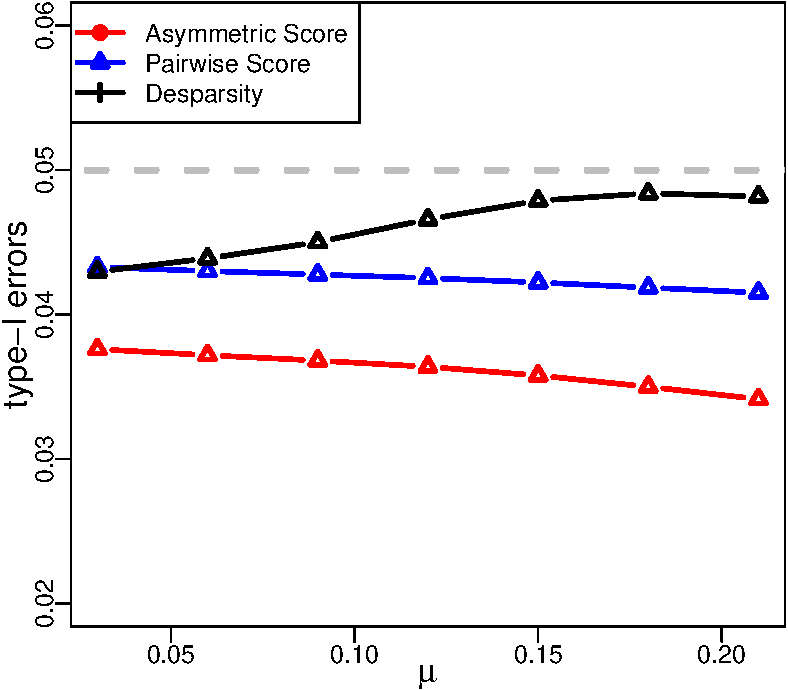
\includegraphics[width=0.35\textwidth]{./figures/GGM_2.pdf}
		&
		\hskip-10pt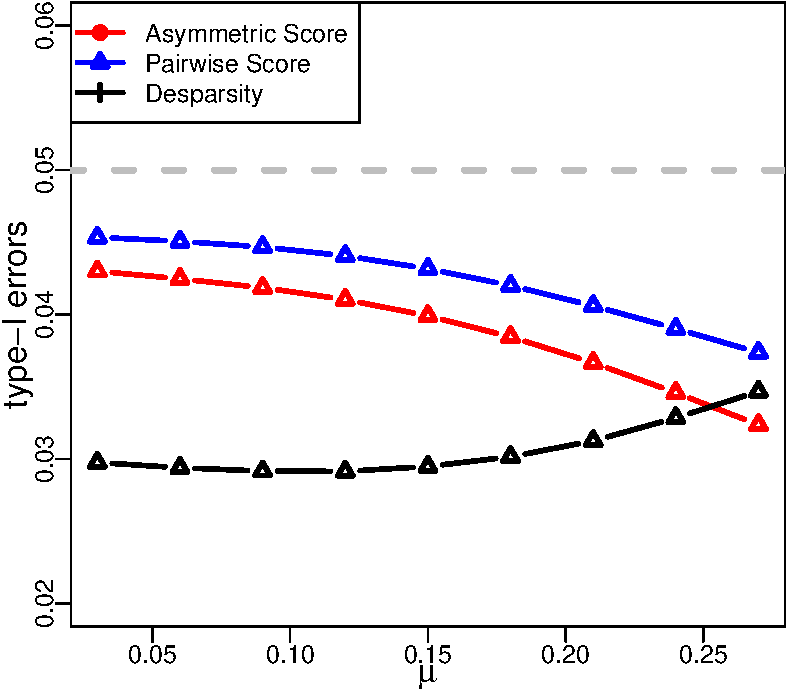
\includegraphics[width=0.35\textwidth]{./figures/Ising_2.pdf}
		&
		\hskip-10pt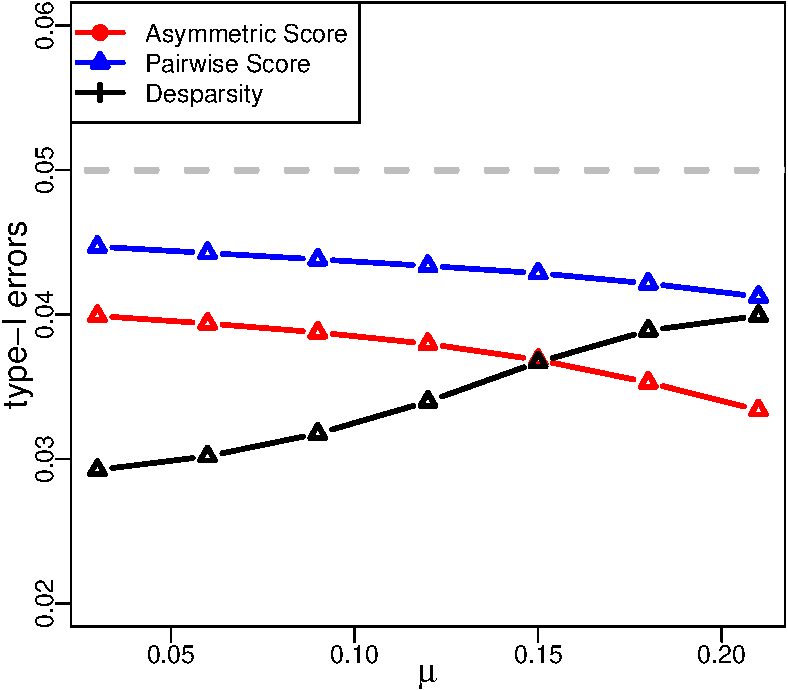
\includegraphics[height=0.306\textwidth]{./figures/Mixed_2.pdf}\\
		\hskip-30pt (a). Gaussian graphical model.&(b). Ising model. &(c). Mixed graphical model.\\
	\end{tabular}\\
	\caption{Type-I errors of the composite pairwise score test, asymmetric score test, and the desparsity method for the three graphical models at the $0.05$ significance level. These figures are  based on $100$ independent simulations. }
	\label{fig::type1}
\end{figure}


\begin{figure}[ht]
\centering
\begin{tabular}{ccc}
\hskip-10pt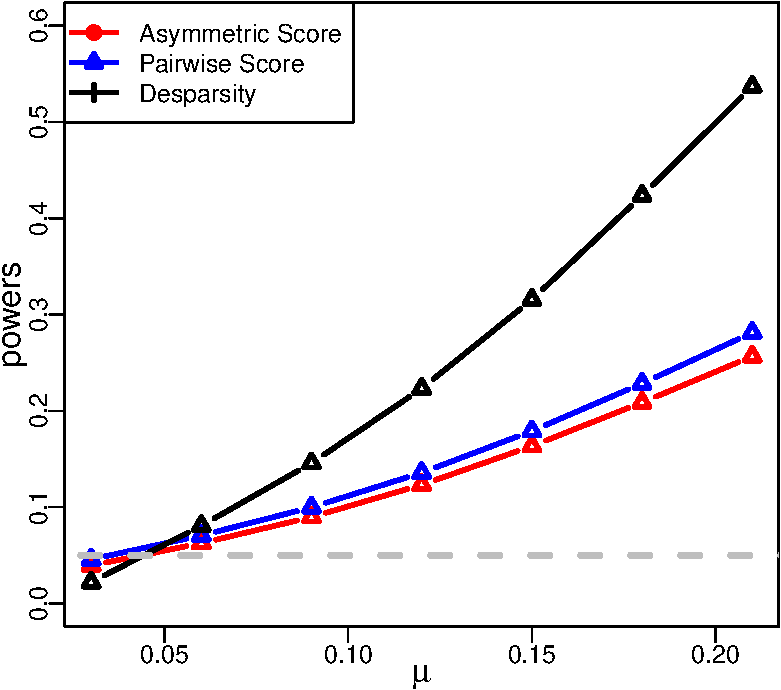
\includegraphics[width=0.35\textwidth]{./figures/GGM.pdf}
&
\hskip-10pt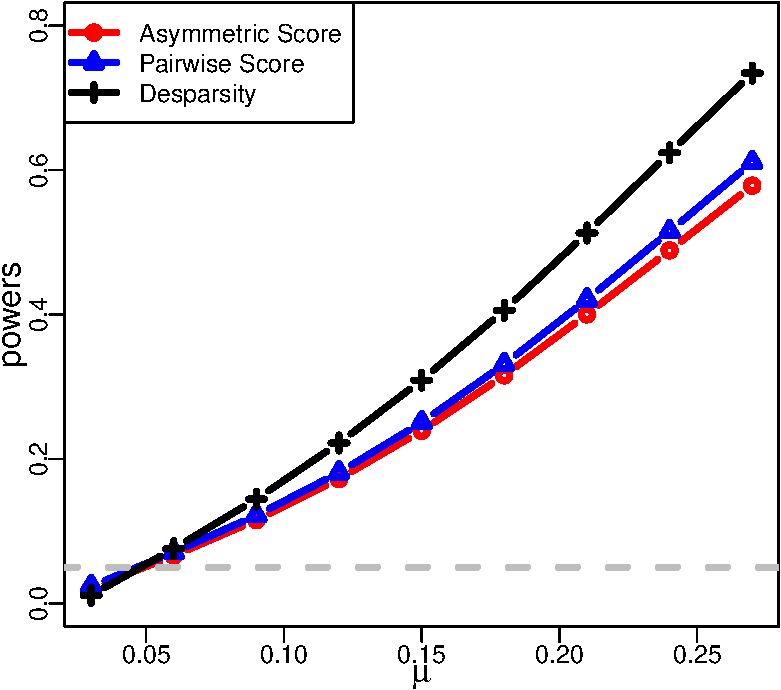
\includegraphics[width=0.35\textwidth]{./figures/Ising.pdf}
&
\hskip-10pt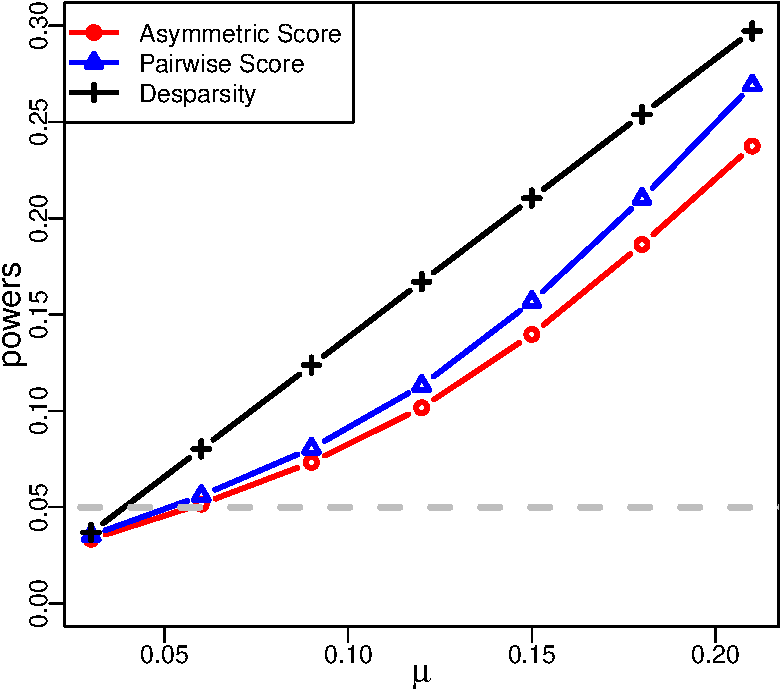
\includegraphics[height=0.309\textwidth]{./figures/Mixed.pdf}\\
\hskip-30pt (a). Gaussian graphical model.&(b). Ising model. &(c). Mixed graphical model.\\
\end{tabular}\\
\caption{Powers   of the composite pairwise score test, asymmetric score test, and the desparsity method for the three graphical models at the $0.05$ significance level. These figures are   based on $100$ independent simulations.}
\label{fig::power}
\end{figure}




%
%
%\begin{table}[ht]
%\begin{center}
%\caption{Local inference results for Gaussian graphical models: Type I errors and Powers of the pairwise score test and the desparsity method \citep{van2013asymptotically}  for $H_0\colon \beta_{jk}^* = 0$ at the $0.05$-significance level. ``Type-I" denotes the type I errors and $\mu$ is the signal strength. }\label{Tab::tab1}
%\begin{tabular}{rrrrrr}
%  \toprule
%  & & \multicolumn{2}{c}{Pairwise Score Test} &\multicolumn{2}{c}{Desparsity Method}\\
%  \cmidrule(r){3-4} \cmidrule(r){5-6}
% & $\mu$& Type-I & Power & Type-I &  Power \\ 
%  \midrule
%1 & 0.00 & 0.051 & 0.051 & 0.049 & 0.049 \\ 
%  2 & 0.03 & 0.051 & 0.068 & 0.055 & 0.078 \\ 
%  3 & 0.06 & 0.053 & 0.100 & 0.050 & 0.118 \\ 
%  4 & 0.09 & 0.056 & 0.159 & 0.052 & 0.188 \\ 
%  5 & 0.12 & 0.056 & 0.242 & 0.051 & 0.284 \\ 
%  6 & 0.15 & 0.052 & 0.432 & 0.055 & 0.496 \\ 
%  7 & 0.18 & 0.054 & 0.623 & 0.050 & 0.691 \\ 
%  8 & 0.21 & 0.053 & 0.724 & 0.052 & 0.781 \\ 
%  9 & 0.24 & 0.054 & 0.793 & 0.047 & 0.861 \\ 
%   \bottomrule
%\end{tabular}
%\end{center}
%\end{table}
%
%
%\begin{table}[ht]
%\centering
%\caption{Local inference results for Ising graphical models: Type I errors and Powers of the pairwise score test and the desparsity method \citep{van2013asymptotically}  for $H_0\colon \beta_{jk}^* = 0$ at the $0.05$-significance level. ``Type-I" denotes the type I errors and $\mu$ is the signal strength.}
%\begin{tabular}{rrrrrr}
%   \toprule
%  & & \multicolumn{2}{c}{Pairwise Score Test} &\multicolumn{2}{c}{Desparsity Method}\\
%  \cmidrule(r){3-4} \cmidrule(r){5-6}
% & $\mu$& Type-I & Power & Type-I &  Power \\ 
%  \midrule
%1 & 0.00 & 0.056 & 0.056 & 0.049 & 0.049 \\ 
%  2 & 0.10 & 0.062 & 0.101 & 0.054 & 0.088 \\ 
%  3 & 0.20 & 0.062 & 0.229 & 0.514 & 0.200 \\ 
%  4 & 0.30 & 0.050 & 0.446 & 0.055 & 0.533 \\ 
%  5 & 0.40 & 0.051 & 0.636 & 0.495 & 0.679 \\ 
%  6 & 0.50 & 0.045 & 0.726 & 0.048 & 0.764 \\ 
%  7 & 0.60 & 0.055 & 0.799 & 0.053 & 0.826 \\ 
%  8 & 0.70 & 0.052 & 0.866 & 0.049 & 0.872 \\ 
%  9 & 0.80 & 0.056 & 0.924 & 0.053 & 0.919 \\ 
%  10 & 0.90 & 0.052 & 0.955 & 0.056 & 0.943 \\ 
%  11 & 1.00 & 0.053 & 0.974 & 0.050 & 0.959 \\ 
%   \bottomrule
%\end{tabular}
%\label{Tab::tab2}
%\end{table}
%
%\begin{table}[ht]
%\centering
%\caption{Local inference results for mixed graphical models: Type I errors and Powers of the pairwise score test and the desparsity method \cite{van2013asymptotically}  for $H_0\colon \beta_{jk}^* = 0$ at the $0.05$-significance level. ``Type-I" denotes the type I errors and $\mu$ is the signal strength.}
%\begin{tabular}{rrrrrr}
%   \toprule
%  & & \multicolumn{2}{c}{Pairwise Score Test} &\multicolumn{2}{c}{Desparsity Method}\\
%  \cmidrule(r){3-4} \cmidrule(r){5-6}
% & $\mu$& Type-I & Power & Type-I &  Power \\ 
%  \midrule
%  1 & 0.00 & 0.057 & 0.057 & 0.054 & 0.054 \\ 
%  2 & 0.03 & 0.052 & 0.065 & 0.054 & 0.057 \\ 
%  3 & 0.06 & 0.056 & 0.104 & 0.052 & 0.128 \\ 
%  4 & 0.09 & 0.053 & 0.133 & 0.050 & 0.147 \\ 
%  5 & 0.12 & 0.050 & 0.219 & 0.046 & 0.253 \\ 
%  6 & 0.15 & 0.051 & 0.398 & 0.059 & 0.425 \\ 
%  7 & 0.18 & 0.058 & 0.592 & 0.052 & 0.589 \\ 
%  8 & 0.21 & 0.058 & 0.687 & 0.054 & 0.729 \\ 
%  9 & 0.24 & 0.053 & 0.753 & 0.050 & 0.786 \\ 
%   \bottomrule
%\end{tabular}
%\label{Tab::tab3}
%\end{table}
%
%
%


\subsection{Real Data Analysis}
We then apply the proposed methods to analyze a publicly available dataset named \texttt{Computer Audition Lab 500-Song (CAL500)} dataset \citep{turnbull2008semantic}. The data can be obtained from the \texttt{Mulan} database \citep{tsoumakas2011mulan}. The \texttt{CAL500} dataset consists of $502$ popular music tracks each of which is annotated by at least  three listeners. The attributes of this dataset include two subsets: (\rmnum{1}) continuous numerical  features extracted from the time series of the audio signal and (\rmnum{2}) discrete binary labels assigned by human listeners to give semantic descriptions of the song. For each music track,  short time Fourier transform is implemented for a sequence of half-overlapping $23$ms time windows over the song's digital audio file. This procedure generates four types of continuous features: \textit{spectral centroids, spectral flux, zero crossings} and a time series of Mel-frequency cepstral coefficient (MFCC).  For the MFCC vectors, every consecutive $502$ short time windows are  grouped together as a block window to produce the following four types of features: (\rmnum{1}) overall mean of MFCC vectors in each block window, (\rmnum{2}) mean of standard deviations of MFCC vectors in each block window, (\rmnum{3}) standard deviation of the means of  MFCC vectors in  each block window, and (\rmnum{4}) standard deviation of the standard deviations of MFCC vectors in each block window.  More details on the feature extraction can be found in  \cite{tzanetakis2002musical}. In addition to  these continuous variables, binary variables in the \texttt{CAL500} dataset include a $174$-dimensional array indicating the existence of each annotation.    These $174$ annotations can be grouped into six categories: emotions ($36$ variables), instruments (33), usages (15), genres (47), song characteristics (27)
and vocal types (16). %In summary, the \texttt{CAL500} dataset consists of $502$ instances with $68$ continuous variables and $174$ binary variables. 
Our goal is to infer the association between these different types of variables using graphical models. This dataset has been analyzed in \cite{cheng2013high} where they exploit a nodewise group-LASSO regression  to estimate the graph structure. In what follows, we use the proposed pairwise score test to examine the graph structure.

%We model the  \texttt{CAL500} dataset using the semiparametric exponential family graphical model. 
Similar to \cite{turnbull2008semantic} and \cite{cheng2013high}, we only keep the MFCC features because they can be interpreted as the amplitude of the audio signal and the other continuous features are not readily interpretable. Unlike \cite{cheng2013high}, we keep all the binary labels. Thus the processed dataset has $n=502$ data points of dimension $d=226$ with $52$ continuous variables and $174$ binary variables.   We apply the pairwise score test to each pair of variables to determine the presence of an edge between them.  The p-values for the null hypothesis that two variables are conditionally independence given the rest of variables are calculated.  
We then apply the Bonferroni  correction to control the familywise error rate at $0.05$.
We set the nonconvex penalty function in optimization problem \eqref{equ::concave} to be capped-$\ell_1$ penalty $p_{\lambda}(u) = \lambda \min\{u,\lambda\}$ with the regularization parameter $\lambda$ selected by $10$-fold cross-validation as in the previous section. 
%For numerical stability, in our analysis, we perform the above testing method $100$ times on randomly drawn  subsamples of size $n/2$ and report the edges selected at least 90 times. 

We compare the pairwise score test with the desparsity  method and the asymmetric score test, which are constructed in the same way as in the simulation. 
We present the fitted graphs obtained by these three methods  in Figure \ref{fig::real_data}-(a)--(c),  where we plot the connected components and omit the singletons. Moreover, in  Figure \ref{fig::real_data}-(d), we plot the intersection of these three graphs.
To better display the graphical structure, we use a square to represent each type of 13 MFCC features respectively. If a node is connected to any node within the group of variables in a MFCC node, then we draw an edge.  We use circles to represent the binary variables and use different colors to indicate their categories. 
The obtained graphs have some interesting properties.  
While all three tests create different graphs, the graphs  obtained by  the pairwise score  test and  the asymmetric score test  have more common edges, which agrees with our simulation results. Indeed, our test can correct the  inconsistency of the asymmetric score test, in the sense that the asymmetric score tests for $\beta_{jk}^*=0$ and $\beta_{kj}^*=0$ may yield different test results. To show this inconsistency problem, we also plot the graph obtained by the asymmetric score test based on the loss function $L_k(\bbeta_k)$ in Figure \ref{fig:real2} in the appendix. Comparing with Figure \ref{fig::real_data}-(b), we can see that the asymmetric score test  indeed leads to many contradictory edges.  

In Figure \ref{fig::real_data}, both the pairwise score test and this  asymmetric score test  discover that songs that are danceable (circle 92) are suited for parties (circle 93), but such a connection is not found by the desparsity method.    This is also true for the connection between  the rapping vocals (circle 119) and the   rap genre (circle 48) and the edge between  strong vocals (circle 122) and  songs with strong emotions (circle 19).   Moreover, in all  three graphs, the continuous features are densely connected within  themselves, which is  similar to the results in \cite{cheng2013high}. All three tests find that the noisiness of the music (square 4) is connected with the quality of songs (circle 85). Furthermore, the common edges  connecting two binary variables also display interesting patterns. For instance, we find that awakening emotions (circle 6) are  connected with soothing  emotions (circle 8); laid-back emotions (circle 14) are  connected with  songs with high energy (circle 32);  sad emotions (circle 20) are  connected with songs with positive feelings (circle 84);  songs with female lead vocals (circle 62) are connected with those with male lead vocals (circle 66). In addition, songs using drum sets (circle 59)  are connected with the electronica genre (circle 46), which is also connected with the acoustic texture (circle 88). %The acoustic texture (circle 88) and the electric texture (circle 89) are also connected. 
All these edges have fairly intuitive explanations. 

In summary, the proposed method reveals some interesting associations between these variables and can be used as a useful complement to analyze high dimensional datasets with more complex distributions.



\begin{figure}[h!]
\centering
\begin{tabular}{cc}
\hskip-30pt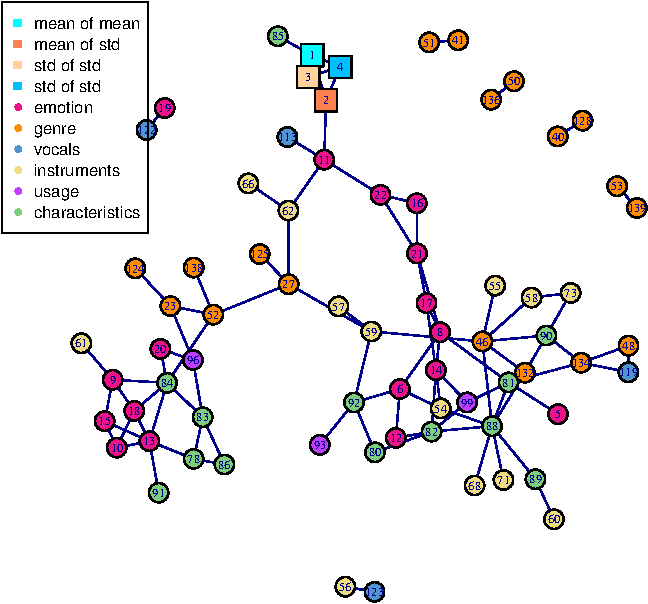
\includegraphics[width=0.49\textwidth]{./figures/real_sym.pdf}
&
\hskip-0pt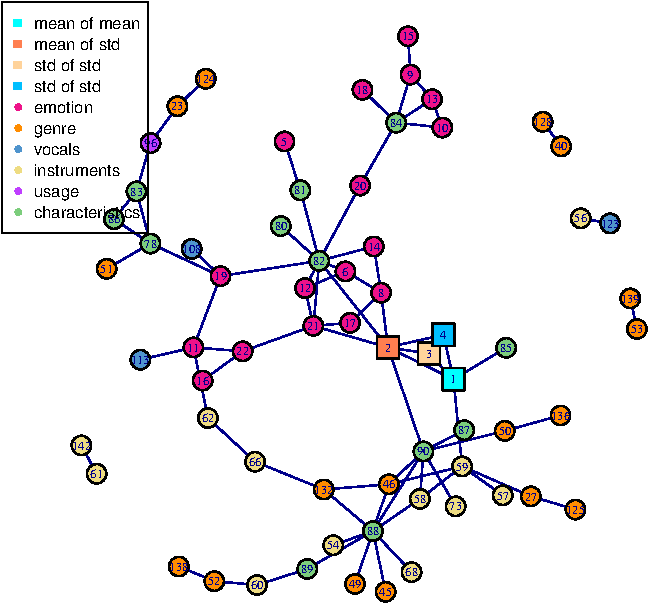
\includegraphics[width=0.49\textwidth]{./figures/real_asym.pdf}\\
\hskip-30pt (a). Pairwise score test.&(b). Asymmetric score test.\\
\hskip-30pt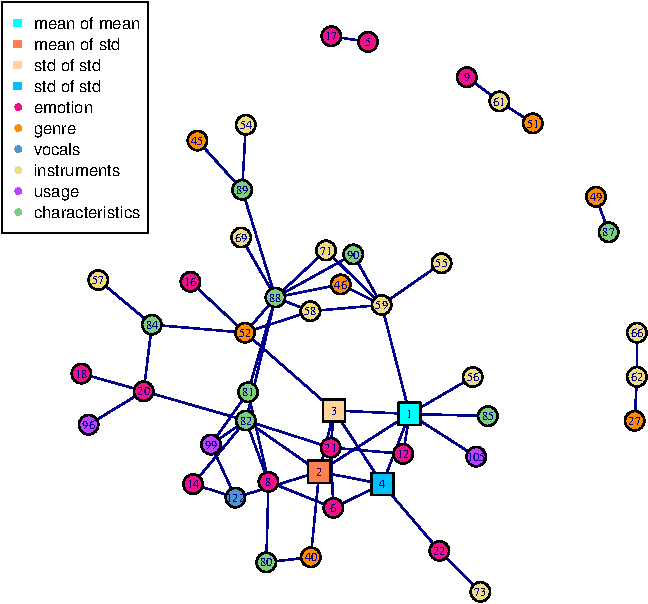
\includegraphics[width=0.49\textwidth]{./figures/real_de.pdf}
&
\hskip-0pt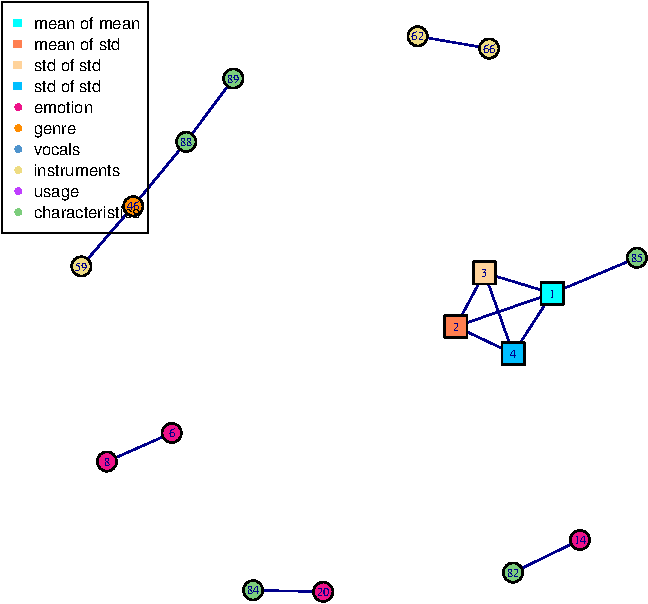
\includegraphics[width=0.49\textwidth]{./figures/intersect123.pdf}\\
\hskip-30pt (c). Desparsity method. &(d). The common edges.\\
\end{tabular}\\
\caption{Estimated graphs in the \texttt{CAL500} dataset inferred by the pairwise score test, asymmetric score test, and the desparsity method. We plot the connected components of the estimated graph. In (a)-(c) we plot the graphs obtained by these three approaches, respectively, and plot the common edges in (d). For better illustration, we only plot the connected components,  combine the same type of continuous variables, display them as a square and draw each binary variable as a circle. The edges of the estimated graph show the association between these variables. }
\label{fig::real_data}
\end{figure}


 

 
\section{Conclusion}\label{sec::conclusion}
We propose an integrated framework for uncertainty assessment of a new  semiparametric exponential family graphical model. The novelty of our model is that the base measures  of each nodewise conditional distribution are treated as unknown nuisance functions. Towards the goal of uncertainty assessment, we first adopt the adaptive multi-stage relaxation algorithm to perform the parameter estimation. Then we propose a composite pairwise score test of the graph structure. 
%function to test whether a given graph contains the true graph. 
Our method provides a rigorous justification for the uncertainty assessment, and is further supported by extensive numerical results. In a followup paper \citep{tan2016replicates}, the proposed model is further extended to account for the unobserved latent variables in the graphical model. 


















% Acknowledgements should go at the end, before appendices and references

\acks{
The authors are grateful for the support  of NSF CAREER Award DMS1454377, NSF IIS1408910, NSF IIS1332109, NIH R01MH102339, NIH R01GM083084, and NIH R01HG06841.
}

% Manual newpage inserted to improve layout of sample file - not
% needed in general before appendices/bibliography.

\newpage

\appendix
 
\section{Proof of the Main Results}
In this appendix we lay out the proof of the main results. In \S \ref{sec::proof_rates} we prove the result of parameter estimation. The proof is based an induction argument that Algorithm \ref{algo::multi} keeps penalizing  most of the irrelevant features and gradually reduces the bias in relevant features.

\subsection{Proof of Theorem \ref{thm::l2rate}}\label{sec::proof_rates}

\begin{proof} 
We only need to  prove the theorem for one node $j\in [d]$, the proof is identical for the rest. 
To begin with, we first define a few index sets that play a significant role in our analysis.
For all $j\in[d],$ we let $ S_j\defeq  \{(j,k)\colon \beta_{jk}^* \neq 0, k\in[d]\}$ be the support of $\bbetas_j.$
For the number of iterations $\ell = 1,2,\ldots$, let $G_{j}^{\ell} \defeq \bigl \{(j,k) \notin S_j\colon \lambda_{jk}^{(\ell-1)} \geq p_{\lambda}'(c_2\lambda),k\!\in\![d]\bigr \} $.  By condition (C.3) of the penalty function $p_{\lambda}(u)$ (see \S\ref{subsec::estimation}), we have $p_{\lambda}'(c_2 \lambda) \geq 0.91\lambda.$ In addition, we let  $J_{j}^{\ell} $ be the largest  $k^*$ components of $\bigl[\hbbeta_{j}^{(\ell)}\bigr]_{G_{j}^{\ell}}$ in absolute value where $k^*$ is defined in Assumption \ref{assume::sparseEig}.
In addition, we let $I_{j}^\ell = ({G_{j}^\ell})^c \cup J_{j}^\ell.$  Moreover, for notational simplicity, we denote $\bigl[\bbeta_j \bigr]_{G_j^\ell},\bigl[\bbeta_j \bigr]_{G_j^\ell}$ and $\bigl[\bbeta_j \bigr]_{I_j^\ell}$ as $\bbeta_{G_j^\ell}, \bbeta_{J_j^\ell}$ and $\bbeta_{I_j^\ell}$ respectively when no ambiguity arises.

The key point of the proof is to show that the complement of $G_j^\ell$ is not too large. To be more specific, we show that $\bigl|(G_{j}^\ell)^c \bigr|\leq 2s^*$ for $\ell \geq 1.$ Since $S_j \subset (G_{j}^\ell)^c,$ $(G_{j}^\ell)^c \leq 2s^*$ implies  $\bigl| (G_{j}^\ell)^c - S_j \bigr| \leq s^*.$ Note that $G_j^\ell$ is the set of irrelevant features that are heavily penalized in the $\ell$-th iteration of the algorithm, $(G_{j}^\ell)^c - S$ being a small set indicates that the most of the irrelevant features are heavily penalized in each step. We show that $\bigl|(G^{\ell})^c\bigr| \leq 2s^*$ for each $\ell\geq 1$ by induction.
 
For $\ell=1$, we have $G_j^1 = S_j^c$ because $\lambda^{(0)}_{jk} = \lambda$ for all $j,k \in [d].$  Hence $\bigl |(G_j^1)^c\bigr|  \leq  s^*$. Now we assume that $|\bigl(G_j^{\ell}\bigr)^c| \leq 2s^*$  for some  integer $\ell$ and our goal is to prove that  $|\bigl(G_j^{\ell+1}\bigr)^c |\leq 2s^*. $  Our proof is based on three technical lemmas.  The first lemma shows that the regularization parameter $\lambda$ in \eqref{equ::concave} is of the same order as $\|\gradstarss\|_{\infty}$.

\begin{lemma}\label{thm::boundGradient}
Under Assumptions \ref{assume::NodeTail} and \ref{assume::sparseEig}, there exists a positive constants $K$  such that, it holds with probability at least $1- (2d)^{-1}$ that 
\begin{flalign}\label{equ::thmGradient}
&\big\|\nabla L_j(\bbeta_j^*)\big\|_{\infty} \leq  K\sqrt{\log d/n}, ~~\forall j\in [d].
\end{flalign}
\end{lemma}
 \begin{proof}  See \S \ref{sec::proof_boundGradient} for a proof.
 \end{proof}
 By this lemma, we conclude that the regularization parameter $\lambda \geq 25 \big\|\nabla L_j(\bbeta_j^*)\big\|_{\infty} $ with high probability. The following lemma bounds the $\ell_1$- and $\ell_2$-norms of $\hbbeta_j ^{(\ell) }\!-\!\bbetas_j $ by the norms of  its subvector under the induction assumption that $\bigl| ( G_j^\ell)^c\bigr| \leq 2s^*.$
\begin{lemma}\label{lemma::BoundByPart}
Letting the index sets $S_{j}, G_{j}^\ell, J_{j}^\ell$ and $I_j^\ell$ be defined as above,  we denote $\tilde G_j^\ell \defeq \bigl( G_j^\ell\bigr)^c.$  Under the assumption that $| G_j^\ell | \leq 2s^*$, we have 
\begin{align}
 \bigl \| \hbbetas^{(\ell)} - \bbetass\bigr \|_2 \leq  2.2\bigl \|  \hbbeta^{(\ell)}_{I_j^{\ell}} -  \bbetas _{I_j^{\ell}}\bigr \|_2~~\text{and}~~
 \bigl \| \hbbetas^{(\ell)} - \bbetass\bigr \|_1 \leq 2.2\bigl \| {\hbbeta}_{\tilde G_j^\ell}^{(\ell)} - \bbetas_{{\tilde G_j}^\ell}\bigr \|_1.
 \label{equ::IBound}
\end{align}
\end{lemma}
\begin{proof} See \S \ref{proof::lemma::BoundByPart} for a detailed proof.
\end{proof}
The next lemma guarantees that $\hbbeta_j^{(\ell)}$ stays in the $\ell_1$-ball centered at $\bbetas_j$ with radius $r$ for $\ell \geq 1$ where $r$ appears in Assumption \ref{assume::sparseEig}.  Moreover, by showing this property of  Algorithm \ref{algo::multi} , we obtain a crude rate for parameter estimation. We summarized this  result in the next lemma.
\begin{lemma} \label{lemma::StayInL1Ball}
For $\ell \geq 1$ and $j\in [d],$ we denote $\blambda_{S_j}^{(\ell)} \coloneqq (\lambda_{jk}^{(\ell)},(j,k)\in S_j)^T$. Assuming that $\bigl | (G_j^{\ell })^c\bigr|\leq 2s^*,$ it holds with probability at least $1- d^{-1}$ that, for all $j \in [d]$, the estimators $\hbbeta_j^{(\ell)}$ obtained in each iteration of  Algorithm \ref{algo::multi}  satisfy \begin{align}\label{equ::TwoNormIneq}
\bigl \| \hbbeta_{I_j^\ell}^{(\ell)} - \bbetas_{I_j^\ell} \bigr\|_2\leq  10 \rho_* ^{-1} \Bigl [\bigl\|\nabla _{\tilde G_j^\ell} L_j(\bbetas_j) \bigr\|_2 + \bigl\|\blambda_{S_j}^{(\ell-1)}\bigr\|_2 \Bigr],~~\tilde G^\ell_j \defeq (G_j^{\ell })^c.
\end{align}
This implies the  following crude rates of convergence for $\hbbeta_j^{(\ell)}\!\!:$
\begin{align}
\bigl \| \hbbetas^{(\ell)} - \bbetass\bigr \|_2 &\leq  24 \rho_*^{-1}\sqrt{s^*} \lambda~~\text{and}~~\bigl \| \hbbetas^{(\ell)} - \bbetass\bigr \|_1 \leq 33 \rho_*^{-1}s^* \lambda . \label{equ::crudeRate}
\end{align}
\end{lemma}

\begin{proof} 
See \S \ref{proof::lemma::StayInL1Ball} for a detailed proof. 
\end{proof}

Now we show that $\tilde G_j^{\ell+1}\!=\! (G_j^{\ell+1})^c$ satisfies $|\tilde G_j^{\ell+1} |\leq 2s^*,$ which concludes our induction.
Letting $A\defeq (G_j^{\ell+1})^c \!-\!S_j,$ by the definition of $G_j^{\ell+1}$, $(j,k) \in A$ implies that  $(j,k)\notin S_j$ and $p_{\lambda}'\bigl(\bigl |\hat \beta_{jk}^{(\ell)} \bigr|\bigr) \leq p_{\lambda}'(c_2\lambda).$ 
Hence by the concavity of $p_{\lambda}(\cdot)$, for any $(j,k)\in A$, $ \bigl|\hat \beta_{jk}^{(\ell)}\bigr | \geq c_2 \lambda.$ 
Therefore we have 
\begin{align}\label{equ::inductionBound}
\sqrt{|A|}& \leq \big\|\hbbeta_{A} ^{(\ell)}\bigr \|_2\big/ (c_2\lambda)  = \big\|\hbbeta_{A} ^{(\ell)} - \bbetas_{A}\big\|_2\big/ (c_2\lambda) \leq 24\rho _*^{-1}\sqrt{s^*} \big/ c_2\leq \sqrt{s^*},
\end{align}
where the first inequality follows from $|A| \leq \sum_{(j,k)\in A} \bigl|\hat \beta_{jk}^{(\ell)}\bigr |^2 \big/(c_2\lambda)^2.$
Note that \eqref{equ::inductionBound}  implies that $\bigl | (G_j^{\ell+1})^c\bigr| \leq 2s^*.$ Therefore by induction, $\bigl|(G_{j}^\ell)^{c}\bigr| \leq 2 s^*$ for any $\ell \geq 1.$

Now we have shown that for $\ell\geq 1$ and $j\in[d],$ $\bigl|(G_j^\ell)^c\bigr|\leq 2s^*$ and the crude statistical rates \eqref{equ::crudeRate} hold. In what follows, we derive the more refined rates \eqref{equ::L2Rate} and \eqref{equ::L1Rate}.\\

\noindent{\bf A refined bound for  $\bigl\|\hbbetas^{(\ell)}- \bbetass\bigr\|_2$ and $\bigl\|\hbbetas^{(\ell)}- \bbetass\bigr\|_1$:}
For notional simplicity, we let $\bdelta^{(\ell)} = \hbbetas^{(\ell)} - \bbetass$  and omit subscript $j$ in $S_j,G_j^\ell, J_j^\ell$ and $I_j^\ell$. We also denote $\tilde G^\ell \defeq (G^\ell)^c.$  We  first derive a recursive bound that links $ \|\bdelta^{(\ell)}_{I^{\ell}}  \|_2 $ to $ \|\bdelta^{(\ell-1)}_{I^{\ell-1}}  \|_2.$ Note that by \eqref{equ::IBound}, 
$
  \| \bdelta^{(\ell)}  \|_1 \leq 2.2  \| \bdelta^{(\ell)} _{\tilde G^{\ell}}  \|_1 \leq 2.2\sqrt{2s^*}  \| \bdelta^{(\ell)} _{\tilde G^{\ell}} \|_2
$. Hence we only need to control $ \|\bdelta^{(\ell)}_{I^{\ell}}  \|_2 $ to obtain the statistical rates of convergence for $\hbbetas^{(\ell)}.$
 By triangle inequality,  
\begin{align*}
\big\|\nabla_{\tilde G^\ell}L_j(\bbetas_j) \big\|_2  \leq\big\|\nabla_{S} L_j(\bbetas_j)\big\|_2  +  \sqrt{|\tilde G^{\ell} - S|}\big\|\gradstarss\big\|_ {\infty}.
 \end{align*}
Since $\lambda > 25 \bigl \| \gradstarss\bigr \|_\infty$, \eqref{equ::inductionBound} implies that 
\begin{flalign}\label{equ::boundGradG}
&\big\|\nabla_{\tilde G^\ell}L_j(\bbetas_j) \big\|_2  \leq\big\|\nabla_{S} L_j(\bbetas_j)\big\|_2 + \bigl \| \bdelta^{(\ell-1)}_{A}\bigr\|_2\big/ (25  c_2),
\end{flalign}
where $A\defeq( G^{\ell})^c - S \subset I^{\ell}.$
Thus \eqref{equ::boundGradG} can be written as
\begin{flalign}\label{equ::boundGradG2}
&\big\|\nabla_{\tilde G^\ell}L_j(\bbetas_j) \big\|_2  \leq\big\|\nabla_{S} L_j(\bbetas_j)\big\|_2 + \bigl \| \bdelta^{(\ell-1)}_{I^{\ell}}\bigr\|_2\big / (25c_2).
\end{flalign}
Also notice that $\forall \beta_{jk} \in \BR$, if $|\beta_{jk} - \beta_{jk}^*| \geq c_2\lambda$, 
$$
p_{\lambda}'(|\beta_{jk}|) \leq \lambda \leq  |\beta_{jk} - \beta_{jk}^*|\big/c_2;
$$
otherwise we have $|\beta_{jk}^*| -|\beta_{jk}| \leq |\beta_{jk} - \beta_{jk}^*|< c_2\lambda$ and thus  $p_{\lambda}'(|\beta_{jk}|) \leq p_{\lambda}'\bigl(|\beta_{jk}^*| \!-\! c_2\lambda\bigr)$ by the  concavity of $p_{\lambda}(\cdot).$
 Hence the following inequality always holds:
\begin{align}\label{equ::gDirBound}
p_{\lambda}'(|\beta_{jk}|) \leq p_{\lambda}'\bigl(|\beta_{jk}^*| \!-\! c_2\lambda\bigr) + |\beta_{jk} - \beta_{jk} ^*|\big/c_2.
\end{align}
Applying \eqref{equ::gDirBound} to $\hbbetas^{(\ell-1)}$ we have
\begin{align*}
\big\|\blambda_{S}^{(\ell-1)}\big\|_2 &\leq \biggl[\sum\limits_{{(j,k)}\in S} p_{\lambda}'\bigl(|\beta_{jk}^*| \!-\! c_2\lambda\bigr)^2 \biggr]^{1/2} + \biggl[\sum\limits_{(j,k)\in S} |\hat\beta_{jk} ^{(\ell-1)}\!- \!\beta_{jk}^*|^2 \biggr]^{1/2}\Big/c_2,
\end{align*} 
which leads to 
\begin{align}\label{equ::lambdaS}
\big\|\blambda_S^{(\ell-1)}\big\|_2 \leq \Bigl[\sum\limits_{{(j,k)}\in S} p_{\lambda}'\bigl(|\beta_{jk}^*| \!-\! c_2\lambda\bigr)^2 \Bigr]^{1/2} +   \bigl \| \bdelta^{(\ell-1)}_{I^{\ell-1}}\bigr\|_2\big/c_2 .
\end{align} 
By  \eqref{equ::TwoNormIneq}, \eqref{equ::boundGradG2} and \eqref{equ::lambdaS} we  obtain 
\begin{align*}
\bigl \| \bdelta^{(\ell)}_{I^{\ell}} \bigr \|_2 &\leq  10\rho_*^{-1}\bigl[ \big\|\nabla_{S} L_j(\bbetas_j)\big\|_2  +\Upsilon_j  \bigr]+ \gamma \bigl \| \bdelta^{(\ell-1)}_{I^{\ell-1}}\|_2 , 
\end{align*}
where  $\gamma \defeq 11 (c_2\rho_*)^{-1}$ and we define $\Upsilon_j \defeq\bigl[\sum_{{(j,k)}\in S} p_{\lambda}'\bigl(|\beta_{jk}^*| \!-\! c_2\lambda\bigr)^2 \bigr]^{1/2}$ for notational simplicity.
Note that since $c_2 \geq 24\rho_*^{-1},$ we have $\gamma < 1.$ By  recursion we obtain
\begin{align}\label{equ::RecursionIk}
\bigl \| \bdelta_{I^{\ell}}^{(\ell)}\bigr \|_2 \leq 10\varrho\bigl[ \big\|\nabla_{S} L_j(\bbetas_j)\big\|_2  +\Upsilon_j \bigr]+\gamma^{\ell-1} \bigl \| \bdelta_{I^1}^{(1)}\bigr \|_2,
\end{align}
where $\varrho \defeq \rho_*^{-1}\cdot(1-\gamma)^{-1} = c_2 (c_2 \rho_* - 11)^{-1}.$
Using  $\bigl \| \hbbetas^{(\ell)} - \bbetass \bigr \|_2 \leq 2.2 \bigl \| \hbbeta_{I_j^{\ell}}^{(\ell)} - \bbetas_{I_j^{\ell}} \bigr \|_2$,  we can bound $\bigl \| \hbbetas^{(\ell)} - \bbetass \bigr \|_2$ by 
\begin{align*}
\bigl \| \hbbetas^{(\ell)} - \bbetass \bigr \|_2 & \leq 22\varrho\bigl[ \big\|\nabla_{S_j} L_j(\bbetas_j)\big\|_2  +\Upsilon_j \bigr] +2.2 \gamma^{\ell -1} \bigl \| \bdelta_{I_j^1}^{(1)}\bigr \|_2.
\end{align*}
Note that for $\ell=1$, by \eqref{equ::TwoNormIneq} we have 
\begin{align}\label{equ::InitialTwoNorm}
\bigl \| \bdelta_{I_j^1}^{(1)}\bigr \|_2 \leq  10 \rho_{*}^{-1} \sqrt{s^*} \big[\lambda  + \sqrt{2}\bigl \| \nabla L_j(\bbetas_j)\bigr\|_{\infty} \bigr]\leq11 \rho_*^{-1}\sqrt{s^*}\lambda =  c_2 \gamma\sqrt{s^*}\lambda.
\end{align}
then we establish the following bound for $\bigl \| \hbbetas^{(\ell)} - \bbetass \bigr \|_2\colon$
\begin{align}\label{equ::FinalL2Rate}
\bigl \| \hbbetas^{(\ell)} - \bbetass \bigr \|_2 \leq  22\varrho\bigl[ \big\|\nabla_{S_j} L_j(\bbetas_j)\big\|_2  +\Upsilon_j  \bigr] + 2.2c_2\sqrt{s^*} \lambda \gamma^{\ell} .
\end{align}

Similarly,  by $\bigl \| \hbbetas^{(\ell)} - \bbetass \bigr \|_1\leq 2.2 \sqrt{2s^*}\bigl \| \hbbeta_{I_j^{\ell}}^{(\ell)} - \bbetas_{I_j^{\ell}} \bigr \|_2,$ we obtain a bound on  $\bigl \| \hbbetas^{(\ell)} - \bbetass \bigr \|_1\colon$ 
\begin{align}\label{equ::IntermediateL1Rate}
\bigl\|\hbbetas^{(\ell)}- \bbetass\bigr\|_1 \leq  32 \sqrt{s^*} \varrho\bigl[ \big\|\nabla_{S_j} L_j(\bbetas_j)\big\|_2  +\Upsilon_j  \bigr]  + 2.2 \gamma^{\ell-1}\sqrt{2s^*}   \bigl \| \bdelta_{I_j^{1}}^{(1)}\bigr \|_2.
\end{align}
By \eqref{equ::InitialTwoNorm}  we have 
$2.2\sqrt{2s^*} \bigl \| \bdelta_{I_j^{1}}^{(1)}\bigr \|_2 \leq 3.2 c_2 \gamma s^* \lambda,$
then the right-hand side of \eqref{equ::IntermediateL1Rate} can be bounded by
\begin{flalign}\label{equ::FinalL1Rate}
\bigl\|\hbbetas^{(\ell)}- \bbetass\bigr\|_1 \leq32 \sqrt{s^*} \varrho\bigl[ \big\|\nabla_{S_j} L_j(\bbetas_j)\big\|_2  +\Upsilon_j  \bigr] + 3.2 c_2  s^* \lambda\gamma^{\ell} .
\end{flalign}
 Therefore  \eqref{equ::L2Rate} and \eqref{equ::L1Rate} can be implied by \eqref{equ::FinalL2Rate} and \eqref{equ::FinalL1Rate} respectively.
 Moreover, by Lemma \ref{lemma::StayInL1Ball}, we conclude that the statistical rates \eqref{equ::FinalL2Rate} and \eqref{equ::FinalL1Rate} hold for all $j\in[d]$ with probability at least $1-d^{-1}.$
\end{proof}
 
\subsection{Proof of Theorem \ref{thm::score}}\label{sec::proof_score}

\begin{proof} 
We first remind the reader that,  for $1\leq j\neq k\leq d,$ we denote   $$\bbeta_{j\setminus k} \!=\! (\beta_{j1},\ldots, \beta_{jj-1},\beta_{jj+1},\ldots, \beta_{jk-1}, \beta_{jk+1},\ldots,\beta_{jd})^T \in\BR^{d-2},$$    $\bbeta_{j\vee k} \!=\! (\beta_{jk}, \bbeta_{j\setminus k}, \bbeta_{k\setminus j})^T\!\in\!\BR^{2d-3}$  and $\hbbeta_{j\vee k}' \!=\! (0,\hbbeta_{j\setminus k},\hbbeta_{k\setminus j})^T$. In addition, we define $\sigma_{jk}^2 = \bSigma^{jk}_{jk,jk} - 2 \bSigma_{jk,j\setminus k}^{jk} \sw_{j,k} -2 \bSigma_{jk,k\setminus j}^{jk} \sw_{k,j}  + {\sw_{j,k}}\!\!\!\!^T \bSigma_{j\setminus k,j\setminus k} ^{jk}\sw_{j,k} + {\sw_{k,j} }\!\!\!\!^T \bSigma_{k\setminus j,k\setminus j} ^{jk}\sw_{k,j} .$
To prove the theorem our goal is to prove the following two arguments:
\begin{align}\label{eqn::two_arguments}
\limn \max_{j<k} \sqrt{n}\bigl | \hat{S}_{jk}\!- \!S_{jk}(\bbetas_{j\vee k})\bigr |  = 0~~\text{and}~~ \limn \max_{j<k} | \hat\sigma _{jk} - \sigma_{jk} | = 0.
\end{align}
Note that by Lemma \ref{lemma::normality}, $\sigma_{jk}^2$ is the asymptotic variance of $\sqrt{n}/2 \cdot S_{jk}(\bbetas_{j\vee k})$. Thus  combining \eqref{eqn::two_arguments} and Slutsky's theorem yields the theorem.
By the the expression of $S_{jk}(\bbetas_{j\vee k})$ and $\hat S_{jk}$  in \eqref{equ::scoreFun2} and \eqref{equ::score2}, under null hypothesis, for a fixed pair of nodes $j$ and $k$, we have $\hat{S}_{jk}\! - \!S_{jk}(\bbetas_{j\vee k})\! =\!I_{1j}\! +\! I_{2j} \! +\! I_{1k}\! +\! I_{2k}$ where $I_{1j}$ and $I_{2j}$ are defined as 
\begin{flalign*}
 I_{1j}&\defeq  \bigl[\nabla_{jk} L_j(\hbbeta_j')- \nabla_{jk} L_j(\bbetas_j)\bigr] - \hw_{j,k} ^T \bigl[ \nabla_{j\setminus k} L_j(\hbbeta_j') -\nabla_{j\setminus k} L_j(\bbetas_j) \bigr]~~\text{and}\\
I_{2j}&\defeq (\sw_{j,k} - \hw_{j,k})^T \nabla_{j\setminus k} L_j(\bbetas_j);
\end{flalign*}
whereas $I_{1k}$ and $I_{2k}$ are defined by interchanging $j$ and $k$ in $I_{1j}$ and $I_{2j}\colon$ 
\begin{flalign*}
 I_{1k} &\defeq \bigl[ \nabla_{kj} L_k(\hbbeta_k') -\nabla_{jk} L_k(\bbetas_k)\bigr] -  \hw_{k,j} ^T\bigl[ \nabla_{k\setminus j} L_k(\hbbeta_k') -  \nabla_{k\setminus j} L_k(\bbetas_k)\bigr]~~\text{and}\\
 I_{2k} &\defeq ( \sw_{k,j} - \hw_{k,j})^T \nabla_{k\setminus j} L_j(\bbetas_k).
\end{flalign*}
We first bound $I_{1j}.$
Recall that $\hbbeta_j' = (0,\hbbeta_{j\setminus k})^T.$
Note that under the null hypothesis, $\beta_{jk}^* = 0,$ by the Mean-Value Theorem, there exists a $\tbbeta_{j\setminus k} \in \BR^{d-2}$ in the line segment between $\hbbeta_{j\setminus k}$ and $\bbetas_{j\setminus k}$ such that 
\begin{align*}
I_{1j}  = \bigl[\tilde \bLambda_{jk,j\setminus k}   - {\hw_{j,k}}^T\tilde \bLambda_{j\setminus k,j\setminus k}\bigr ] \bigl( \hbbeta_{j\setminus k} - \bbetas_{j\setminus k}\bigr),
\end{align*}
where $\tilde \bLambda \defeq \nabla^2 L_j(0,\tbbeta_{j\setminus k}).$
We let $\bdelta \defeq \hbbeta'_j - \bbetas_j$ and denote $\nabla^2 L_j(\hbbeta'_j)$ and $\nabla^2 (\bbetas_j)$ as $\bLambda$ and $\bLambda^*$ respectively. From the definition of Dantzig selector we obtain
\begin{align*}
|I_{1j}| &\leq  \underbrace{  \|\bLambda_{jk,j\setminus k}  - {\hw}^T\bLambda_{j\setminus k,j\setminus k} \|_{\infty} \| \bdelta_{j\setminus k}\|_1}_{I_{11}}   + \underbrace{  \|\bLambda_{jk,j\setminus k}  - \tilde \bLambda_{jk,j\setminus k} \|_\infty\| \bdelta_{j \setminus k}\|_1}_{I_{12}}\\
  &+  \underbrace{  \|  {\hw}^T (\bLambda_{j\setminus k,j\setminus k}  - \tilde \bLambda_{j\setminus k,j\setminus k}  )\bdelta_{j\setminus k} \|_{\infty}}_{I_{13}}.
\end{align*}
Theorem \ref{thm::l2rate} implies that $\bigl\|\bdelta \|_1 \leq C s^* \lambda$ with probability tending to $1$ for some constant $C>0$.  Then 
by the definition of Dantzig selector, $I_{11}  \leq C s^* \lambda\lambda_D.$ with high probability.
 Moreover, the constant $C$ is the same for all $(j,k).$   By assumption \ref{assume::Dantzig}, $I_{11} = o(n^{-1/2})$ with probability tending to one.

For term $I_{12}$, H\"{o}lder's inequality implies that 
\begin{align}\label{equ::boundI121}
I_{12} \leq   \|\bLambda_{jk,j\setminus k}  -\tilde \bLambda_{jk,j\setminus k} \|_\infty   \| \bdelta_{j \setminus k}   \|_1.
\end{align}
 By  Lemma \ref{lemma::HessOneNode} we obtain 
\begin{align}\label{equ::anotherPertHess}
 & \| \bLambda - \tilde \bLambda  \|_\infty \leq  \| \bLambda - \bLambda ^* \|_\infty  + \|\bLambda ^* - \tilde \bLambda  \|_\infty \leq 2 Cs ^* \lambda \log^2 d.
\end{align}
Therefore  combining \eqref{equ::boundI121} and \eqref{equ::anotherPertHess} we have 
\begin{align*}
I_{12} \leq 2C {s^*}^2  \lambda ^2 \log^2 d \lesssim s^*\lambda \lambda_D\quad \text{uniformly for } 1\leq j < k \leq d.
\end{align*}
Similarly by H\"{o}lder's inequality, we have  
\begin{align}\label{equ::I13bound}
I_{13} \leq  \| \hw_{j,k} \|_1  \| \bLambda - \tilde \bLambda \|_\infty \|\bdelta\|_ 1.
\end{align}
Notice that by the optimality of $\hw_{j,k},$ $ \| \hw_{j,k} \|_1  \leq  \| \sw_{j,k} \|_1 \leq w_0.$ Combining \eqref{equ::I13bound} and \eqref{equ::anotherPertHess} we have
\begin{align*}%\label{equ::I13Bound2}
I_{13} \leq Cw_0{s^*}^2 \lambda^2 \log^2 d\lesssim  s^* \lambda \lambda_D  \quad \text{uniformly for } 1\leq j < k \leq d.
\end{align*}
where we use the fact that $\lambda_D \gtrsim \max\{1,w_0\} s^* \lambda\log^2 d.$
Therefore we  conclude that  for all $j\in [d]$,
$
| I_{1j} | \lesssim s^* \lambda\lambda_D = o_{\PP}(n^{-1/2}).
$
For $I_{2j}$, H\"{o}lder's inequality implies that $| I_{2j} |  \leq   \| \sw _{j,k}- \hw_{j,k}\|_{1} \bigl \| \nabla L_j(\bbetas_j)\bigr \|_{\infty } $. 
To control $\| \sw _{j,k}- \hw_{j,k}\|_{1}$, we need to the following lemma to obtain the estimation error of the Dantzig selector $\hw_{j,k}.$
\begin{lemma}\label{lemma::DantzigRate}
For $1\leq j\neq k\leq d,$  let $\hw_{j,k}$ be the solution of the Dantzig-type optimization problem \eqref{equ::Dantzig} and let ${\sw_{j,k}} = \Hb_{jk, j\setminus k}^{j} (\Hb_{j\setminus k,j\setminus k}^{j})^{-1}$. Under Assumptions \ref{assume::NodeTail}, \ref{assume::sparseEig}, \ref{assume::BoundedHess}  and \ref{assume::Dantzig}, with probability tending to one,
 we have 
$$
  \| \hw_{j,k} - \sw_{j,k}   \|_1\leq 37 \nu_*^{-1} s_0^\star\lambda_D~~\text{for all}~~1\leq j\neq k\leq d.
$$
\end{lemma}
\begin{proof} See \S \ref{proof::lemma::DantzigRate} for a detailed proof.
\end{proof}

Now combining  Lemma \ref{lemma::DantzigRate} and Theorem \ref{thm::boundGradient} we obtain that 
\begin{align*}%\label{equ::boundI2}
| I_{2j} | \leq 37 \nu_*^{-1}K_1 s_0^\star \lambda_{D}\sqrt{\log d/n}\asymp s_0^\star \lambda \lambda_D = o(n^{-1/2}).
\end{align*}
Therefore we have shown that $I_{1j} + I_{2j} = o(n^{-1/2})$ with high probability. Similarly, we also have $I_{1k} + I_{2k} = o(n^{-1/2})$  with high probability.
Moreover, since the bounds for $|I_{1j}|$ and $|I_{2j}|$ is independent of the choice of $(j,k)\in\{ (j,k)\colon 1\leq j\neq k\leq d\}$, we conclude that  
 $$
\sqrt{n} \bigl [\hat{S}_{jk}- S_{jk}\bigl(\bbetas_{j\vee k}\bigr) \bigr]= o_{\PP}(1) \quad \text{uniformly for } 1\leq j < k \leq d.
 $$
 Our next lemma characterizes the limiting distribution of $\gradstarst$ and is pivotal for establishing the validity of the composite pairwise score test.
\begin{lemma}\label{lemma::normality}
For any $\bbb \in \BR^{2d-3}$  with $\| \bbb \|_2 \!=\! 1$ and $ \ | \bbb   \|_0 \leq \tilde s$,  if $\limn \tilde s \big / n\!=\! 0$, we have 
\begin{align}\label{equ::gradNormality}
\sqrt{n}/2 \cdot \bbb^T \nabla L_{jk}\bigl(\bbetas_{j \vee k}) \leadsto N\bigl(0, \bbb^T \bSigma^{jk}  \bbb\bigr).
\end{align}
\end{lemma}

By Lemma \ref{lemma::normality} we obtain
 \begin{align*}
  \sqrt {n}/2\cdot  S\bigl(\bbetas_{j\vee k}\bigr) =\nabla_{jk} L_{jk}\bigl(\bbetas_{j\vee k}\bigr) - {\sw_{j,k}}\!\!\!\! ^T \nabla_{j\setminus k} L_{jk}\bigl(\bbetas_{j\vee k}\bigr) - {\sw_{k,j}}\!\!\!\! ^T \nabla_{j\setminus k} L_{jk}\bigl(\bbetas_{j\vee k}\bigr) \leadsto N(0,\sigma_{jk}^2),
  \end{align*}
where the asymptotic variance $\sigma_{jk}^2$ is given by
 $$\sigma_{jk}^2 = \bSigma^{jk}_{jk,jk} - 2 \bSigma_{jk,j\setminus k}^{jk} \sw_{j,k} -2 \bSigma_{jk,k\setminus j} \sw_{k,j}  + {\sw_{j,k}}\!\!\!\!^T \bSigma_{j\setminus k,j\setminus k} ^{jk}\sw_{j,k} + {\sw_{k,j} }\!\!\!\!^T \bSigma_{k\setminus j,k\setminus j} ^{jk}\sw_{k,j} .$$
 For a more accurate estimation of  $\hat{S}_{jk}- S_{jk}\bigl(\bbetas_{j\vee k}\bigr) $, we have
 \begin{align}\label{equ::UniformConvSbbeta}
\sqrt{n} \bigl |\hat{S}_{jk}- S_{jk}\bigl(\bbetas_{j\vee k}\bigr) \bigr|\leq \sqrt{n} \bigl (   |I_1| +  |I_2| \bigr) \lesssim \sqrt{n} (s^*\! +\! s_0^\star) \lambda \lambda_D . 
\end{align}
 Finally, the following lemma, whose proof is deferred to the supplementary material, shows that $\hat\sigma_{jk} $ is a consistent estimator of $\sigma_{jk}$.
 
 \begin{lemma}\label{lemma::var} For $1\leq j\neq k\leq d$, we denote the asymptotic variance of $\sqrt{n}/2 \cdot S_{jk}(\bbetas_{j\vee k})$ as $\sigma_{jk}^2$. Under  Assumptions \ref{assume::NodeTail}, \ref{assume::sparseEig}, \ref{assume::BoundedHess} and \ref{assume::Dantzig},  the estimator $\hat\sigma_{jk}$  satisfies $\limn \max\limits_{j<k} | \hat\sigma _{jk} - \sigma_{jk} | = 0.$
 \end{lemma}
 \begin{proof} 
 See \S\ref{proof::lemma_var} for a proof.
 \end{proof}
 Since $\hat\sigma_{jk}$ is consistent for $\sigma_{jk}$ by Lemma \ref{lemma::var}  and $\sigma_{jk}$ is bounded away from zero by Assumption \ref{assume::BoundedHess}, Slutsky's theorem implies that $\sqrt{n} \hat{S}_{jk}/(2\hat\sigma_{jk}) \leadsto N(0,1)$.
\end{proof}

\section{Additional Estimation Results}

We present the additional results of parameter estimation. In \S \ref{sec::Sparse_Eig_GGM} we verify the sparse eigenvalue condition for Gaussian graphical models, which justifies Assumption \ref{assume::sparseEig} in our paper. In \S \ref{sec::refined_rates} we derive a more refined statistical rates of convergence for the iterates of Algorithm \ref{algo::multi}.
\subsection{Verify the Sparse Eigenvalue Condition for Gaussian Graphical Models}\label{sec::Sparse_Eig_GGM}
In this subsection, we verify the sparse eigenvalue condition for Gaussian graphical models. Moreover, we show that such condition holds uniformly over a $\ell_1$-ball centered at the true parameter $\bbeta_j^*$.
\begin{proposition}\label{prop::SparseEigGGM}
 Suppose $\bX\! \sim\! N({\bf 0},\bSigma)$ is a Gaussian graphical model and  let $\bTheta\! =\! \bSigma^{-1}$ be the precision matrix.  For all $j \in [d],$ the conditional distribution of $X_j$ given $\bX_{\setminus j}$ is a normal distribution with mean ${\bbetass}^T \bX_{\setminus j}$ and variance $\bTheta_{jj}^{-1},$ where $\bbetas_j \!=\! \bTheta_{j\setminus j}.$  Let $L_j(\cdot)$ be the loss function defined in \eqref{equ::NodewiseLoss}. We   assume that  there exist positive constants $D,\  c_{\lambda}$ and $C_{\lambda} $ such that  $  \| \bSigma  \|_\infty \leq D$ and  $c_\lambda \leq \lambda_{\min}(\bSigma ) \leq \lambda_{\max} (\bSigma) \leq C _ \lambda.$   We let $s^* \! = \! \max_{j\in[d]} \| \bbetass \|_0 $ and  also assume that  there exists a constant $C_{\beta}>0$ such that $  \| \bbetass   \| _2 \leq C _\beta$  for all $j\in [d].$ Suppose $r>0$ is a real number such that $r = \cO( 1/\sqrt{s^*})$. Then, there exist $\rho_*, \rho^* >0$ such that   for all $j\in [d],$ and $s = 1,\ldots,d-1,$
 \begin{align*}
 \rho_*  \leq \rho_{-}\bigl(\EE \bigl[\nabla^2 L_j \bigr], \bbetass ; s,r\bigr) \leq \rho_{+}\bigl(\EE  \bigl[\nabla^2 L_j \bigr], \bbetass ; s,r\bigr) \leq \rho^*.
 \end{align*}
 \end{proposition}

\begin{proof} 
We prove this lemma in two steps. For any $\bbeta_j\in \BR^{d-1 }$ such that $ \| \bbeta_j - \bbetas_j \|_1 \leq r$ and any $\vb\in\BR^{d-1}$ such that $\| \vb\|_2 = 1,$  we first give a lower bound for $\vb^T \EE \bigl[\nabla^2 L_j(\bbeta_j)\bigr] \vb$ by truncation. Then we give an upper bound in the second step.

\vspace{5pt}
\noindent{\bf Step (\rmnum{1}): Lower Bound of $\vb^T \EE \bigl[\nabla^2 L_j(\bbeta_j)\bigr] \vb$.} We denote $\mathbb{B}_j(r)\coloneqq \bigl\{ \bbeta\in \BR^{d-1}\colon  \| \bbeta- \bbetas_j \|_1 \leq r\bigr\}$. For two truncation levels  $\tau >0$ and $R >0$, we denote
 $\cA_{ii'} \defeq \bigl \{ | X_{ij} | \leq \tau \bigr\}  \cap \bigl \{ | X_{i'j} | \leq \tau \bigr\} $, $\cB_{i} \defeq  \bigl \{\bigl | \bX_{i \setminus j}^T \bbeta_j\bigr |\leq R, \forall \bbeta_j\in \BB_j(r)\bigr  \} $ 
 and $\cB_{i'} \defeq \bigl \{ \bigl | \bX_{i'\setminus j}^T \bbetass\bigr| \leq R, \forall \bbeta_j\in \BB_j(r)\bigr  \}.$   The values of $R$ and $\tau$ will be determined later. 
 By the definition of $L_j(\cdot), $ for any $\bbeta_j \in \BB_j(r)$ and any $\vb \in \BR^{d-1}$ with $\| \vb \|_2 =1 $, we have 
\begin{align}\label{equ::TheresholdHess}
\vb^T \nabla^2 L_j (\bbeta_j  ) \vb  \geq \frac{2C_1(R,\tau)}{n(n-1)} \sum_{i<i'} \bigl (X_{ij} - X_{i'j}\bigr) ^2  \bigl [\bigl(\bX_{i\setminus j} - \bX_{i' \setminus j}\bigr)^T \vb \bigr]^2 I(\cB_i)T(\cB_{i'})  I ( \cA_{ii'}), 
\end{align}
where $C_1(R,\tau) \defeq \exp(-4R\tau) \bigl[1  + \exp(-4R\tau)\bigr]^{-2}.$ For notational simplicity, we denote the right-hand side of \eqref{equ::TheresholdHess} as $C_1(R,\tau)\vb^T \bDelta\vb.$ By the properties of Gaussian graphical models, the conditional density of $X _{ij}$ given $\cI _i\defeq \bigl\{ \bX_{i\setminus j} = \bx_{i\setminus j}\bigr \} \cap \cB_i $
 is 
 \begin{align*}
 p\bigl(x_{ij} |\cI_i)  = p(\bx_i | \cB_i)\Big / \int _{\BR } p(\bx_i | \cB_i) \ud x_{ij} =  p(x_{ij}| \bx_{i \setminus j}),
 \end{align*}
 where we use the fact that $p(\bx_i | \BB_i) = p(\bx_i) / \PP(\cB_i)$ and that $\PP(\cB_i)$ is a constant.
 Recall that $$p(x_{ij}| \bX_{i \setminus j})  =\sqrt{ \bTheta_{jj}\big/( 2\pi)} \exp \bigl [- \bTheta_{jj}/2  (x_{ij} - \bX_{i \setminus j}^T \bbetas_{j}  )^2  \bigr ]~~\text{where}~ \bbetas_j = \bTheta_{j\setminus j}.$$ 
 Thus the conditional expectation of $(X_{ij} - X_{i'j})^2   I ( \cA_{ij})$ given $\cI_{i}$ and $\cI_{i'}$ is
 \begin{flalign*}
 &\EE \Bigl [(X_{ij} - X_{i'j})^2   I ( \cA_{ii'}) \Big | \cI_{i} \cap \cI_{i'}\Bigr ] \notag\\
  & \quad =    \bTheta_{jj} / (2\pi) \int _{-\tau} ^{\tau} \int _{-\tau} ^{\tau}   (x_{ij}- x_{ij})^2 \exp\Bigl \{ -\bTheta_{jj}/2 \bigl[ (x_{ij} - \bbeta_j ^T \bx_{i\setminus j} )^2 + (x_{i'j} - \bbeta_j^T \bx_{i'\setminus j} )^2 \bigr ]   \Bigr \} \ud x_{ij} \ud x_{i'j}.
 \end{flalign*}
 Note that on event $\cI_i,$ $| \bbeta_j ^T \bX_{i\setminus j}  | \leq R,$ hence the expression above can be lower-bounded by 
 \begin{flalign*}
 & \EE \Bigl [(X_{ij} - X_{i'j})^2   I ( \cA_{ii'}) \Big | \cI_i \cap \cI_{i'}\Bigr ] \notag\\
 & \quad \geq  \bTheta_{jj} / (2\pi) \int _{-\tau} ^{\tau} \int _{-\tau} ^{\tau}   (x_{ij}- x_{i'j})^2 \exp\Bigl \{ -\bTheta_{jj}/2 \bigl[x_{ij}^2 + x_{i'j}^2  +2R^2 + 2R (| x_{ij} | +| x_{i'j} |) \bigr]   \Bigr \} \ud x_{ij} \ud x_{i'j}.
 \end{flalign*}
The last expression is positive and we denote it as $C_2(R,\tau) $ for simplicity. Thus by the law of total expectation we obtain 
\begin{flalign*}
& \vb ^T \EE(\bDelta ) \vb  = \vb^T \EE \bigl [ \EE  (\bDelta \big | \cap _{i=1}^n \cI_i ) \bigr ]\vb \geq   C_2(R,\tau) \EE \Bigl\{ \bigl[ (\bX_{i\setminus j} - \bX_{i' \setminus j})^T \vb   \bigr]^2I(\cB_i)I(\cB_j)\Bigr \}.
\end{flalign*}
By Cauchy-Schwarz inequality we have 
\begin{align}\label{equ::BoundUseCauchy}
\EE \Bigl \{ \bigl [(\bX_{i\setminus j} - \bX_{i' \setminus j})^T \vb \bigr ]^2 \bigl[ 1- I(\cB_{i})I(\cB_{i'}) \bigr]\Bigr \} \leq \sqrt{ \EE [(\bX_{i\setminus j} - \bX_{i' \setminus j})^T \vb \bigr ]^4 } \sqrt{  \PP\bigl (  \cB_i^c \cup \cB_{i'}^c \bigr ) }.
\end{align}
Note that for Gaussian graphical model, the marginal distribution of  $\bX_{\setminus j}$ is $N({\bf 0},\bSigma_{\setminus j\setminus j}) $. If we denote $\bSigma_{\setminus j\setminus j}$ as $\bSigma_1,$ we have  $(\bX_{i\setminus j} \!-\! \bX_{i' \setminus j})^T \vb \sim N({\bf 0}, \sigma_v^2  )  ,$ 
$\bX_{i\setminus j} ^T \bbetas_{j} \sim N({\bf 0},\sigma_1^2 )$   
and $\bX_{i\setminus j}^T \bbeta\sim N({\bf 0},\sigma_2^2 )$  where $\sigma_v^2 \!=\!2 \vb^T\bSigma_1 \vb,$  $\sigma_1 ^2\! =\!  {\bbetas_{j}}^T \bSigma_1 \bbetas_{j} $ 
and $\sigma_2 ^2 \!=\! \bbeta_j^T \bSigma_1 \bbeta_j.$ 
Hence we have $\EE \bigl[(\bX_{i\setminus j} - \bX_{i' \setminus j})^T \vb \bigr]^4 = 3\sigma_v ^4.$
Because the maximum eigenvalue of $\bSigma_1$ is upper bounded by $C_\lambda$,  we have 
$
\sigma_1^2 \leq  C_\lambda C _\beta^2
$
 and $\sigma_v ^2\leq 2C_\lambda.$
 Note that $\sigma_2^2 \!-\! \sigma_1^2\! =\! \bbeta_j^T \bSigma_1 \bbeta_j \!-\!  {\bbetas_{j}}^T \bSigma_1 \bbetas_{j},$ the following lemma in linear algebra bounds this type of error. 
 
\begin{lemma}\label{lemma::SymmetricDiff}
Let $ \Mb \in \BR ^{d\times d}$ be a symmetric matrix and vectors $\vb_1$ and $\vb_2 \in \BR^d$, then
$$
\bigl |\vb_1^T \Mb \vb_1 - \vb_2^T \Mb \vb_2\bigr|\leq  \|\Mb \|_{\infty}  \|\vb_1- \vb_2 \|_1^2 + 2  \|\Mb \vb_2 \|_{\infty}  \|\vb_1- \vb_2 \|_1.$$
\end{lemma}
\begin{proof} 
Note that $\vb_1^T \Mb \vb_1 - \vb_2^T \Mb \vb_2 = (\vb_1 \!-\! \vb_2)^T \Mb(\vb_1\! -\! \vb_2 ) + 2 \vb_2^T\Mb(\vb_1\! -\! \vb_2),$ H\"older's inequality implies 
\$
\bigl |\vb_1^T \Mb \vb_1 - \vb_2^T \Mb \vb_2\bigr | &\leq\bigl |(\vb_1 \!-\! \vb_2)^T \Mb(\vb_1\! -\! \vb_2 )\bigr| +2\bigl|\vb_2^T\Mb(\vb_1\! -\! \vb_2)\bigr|\\
&\leq \|\Mb \|_{\infty}  \|\vb_1- \vb_2 \|_1^2 + 2  \|\Mb \vb_2 \|_{\infty}  \|\vb_1- \vb_2 \|_1.
\$
Hence, we conclude the proof of Lemma \ref{lemma::SymmetricDiff}.
\end{proof}
By Lemma \ref{lemma::SymmetricDiff}, we have
\begin{align}\label{equ::varianceDiff}
\sigma_2^2 - \sigma_1 ^2 \leq  \| \bSigma _1 \|_\infty  \| \bbeta_j -  \bbetass\bigr \|_1^2 + 2  \| \bSigma_1 \bbetass   \|_\infty  \| \bbeta_j -  \bbetass \|_1.
\end{align}
By H\"older's inequality and the relation between $\ell_1$-norm and $\ell_2$-norm of a vector, we have $  \| \bSigma_1 \bbetass \|_\infty \leq   \| \bSigma_1   \|_\infty   \|\bbetass   \|_1 \leq \sqrt{s^*} C_\beta D.
$
Therefore  the right-hand side of \eqref{equ::varianceDiff} can be bounded by 
\begin{align*}
\sigma_2^2 - \sigma_1 ^2 \leq r^2 D + 2 \sqrt{s^*} r C_\beta D,
\end{align*}
which shows that $\sigma_2^2$ is also bounded because $r=\cO(1\big/\sqrt{s^*}).$
 In addition, by the bound  $1- \Phi(x) \leq \exp(-x^2/2) / (x\sqrt{2\pi})$ for the standard normal distribution function, we obtain that
\begin{align*}
& \PP \bigl ( \cB_i^c\bigr) \leq  \PP\bigl (  \bX_{i \setminus j}^T \bbetas _{j}  > R \bigr )+\PP\bigl ( \bX_{i \setminus j}^T \bbeta_j >R\bigr ) \notag \\
& \quad   \leq  c \sigma_1 \exp\bigl[-R^2 /( 2\sigma_1^2)\bigr] /R + c\sigma_2 \exp\bigl[  -R^2 /( 2\sigma_2^2)\bigr]/R,
\end{align*} 
where the constant $c = 1/\sqrt{2\pi}.$ We denote the last expression as $C_3(R),$ then the right-hand side of \eqref{equ::BoundUseCauchy} can be upper-bounded by $ \sqrt{ 3 \sigma_v^4} \sqrt{ 2 C_3(R) } \leq 2\sqrt{6C_3(R)} C_\lambda .$ 
 Hence we can choose a sufficiently large $R$ such that $2\sqrt{6C_3(R)} C_\lambda= \lambda_{\min}(\bSigma)$ and we denote this particular choice of $R$ as $R_0.$

Now we have 
$$
\EE \Bigl \{ \bigl [(\bX_{i\setminus j} - \bX_{i' \setminus j})^T \vb \bigr ]^2 \bigl[ 1- I(\cB_{i})I(\cB_{i'}) \bigr]\Bigr \} \leq \lambda_{\min}(\bSigma)
$$
Note that $\EE \bigl \{ [(\bX_{i\setminus j} - \bX_{i' \setminus j})^T \vb ]^2\bigr\}  = \sigma_v^2 \geq 2 \lambda_{\min}(\bSigma),$
 we obtain that $$\vb^T \EE \bigl[  \nabla^2 L_j(\bbeta_j )\bigr] \vb \geq C_1(R_0,\tau) C_2(R_0,\tau)  \lambda_{\min} ( \bSigma)~~\text{for all}~~ \tau \in \BR.$$ Therefore we conclude that for all $\bbeta_j\in \BR^{d-1}$ such that $ \| \bbeta_j - \bbetass   \|_1 \leq r,$ 
 \begin{align}\label{equ::GGMlower}
 \vb^T \EE \bigl[\nabla^2 L_j(\bbeta_j )\bigl] \vb \geq \max _{\tau\in \BR}\bigl \{ C_1(R_0,\tau) C_2(R_0,\tau)  \bigr\} \lambda_{\min} ( \bSigma).
 \end{align}
 
 \vspace{5pt}
 \noindent{\bf Step (\rmnum{2}): Upper Bound of $\vb^T \EE \bigl[\nabla^2 L_j(\bbeta_j)\bigr]\vb$.} For any $\bbeta_j \in \BR^{d-1}$ such that $ \| \bbeta_j - \bbetass \|_1 \leq r $ and for any $\vb \in \BR^{d-1}$ with $\| \vb \|_2 = 1$, by the definition of $\nabla^2 L_j(\bbeta_j)$  we have 
\begin{align}\label{equ::UpperBoundHess}
\vb^T \nabla^2 L_{j}(\bbeta_j) \vb \leq (X_{ij} - X_{i'j} ) ^2 \bigl [(\bX_{i\setminus j} - \bX_{i' \setminus j})^T \vb \bigr ]^2 .
\end{align}
Notice that conditioning on $\bX_{i\setminus j},$ $X_{ij} \sim N\bigl(\bX_{i \setminus j}^T \bbetass, \bTheta_{jj}^{-1}\bigr),$ hence
\begin{align}\label{equ::ConditionalXs}
\EE\bigl [ (X_{ij} - X_{i'j} ) ^2  \big | \bX_{i\setminus j}, \bX_{i' \setminus j} \bigr ]  = \bigl[ (\bX_{i \setminus j} - \bX_{i' \setminus j})^T \bbetass\bigr ]^2  + 2\bTheta_{jj}^{-1}.
\end{align}
Combining \eqref{equ::UpperBoundHess} and \eqref{equ::ConditionalXs} we obtain 
\begin{flalign}\label{equ::UpperboundExpectation}
& \EE \bigl[ \vb^T \nabla^2 L_j(\bbeta_j) \vb \bigr ] \leq \EE \Bigl \{ \EE  \bigl[ (X_{ij} - X_{i'j} ) ^2  \big | \bX_{i\setminus j}, \bX_{i' \setminus j} \bigr ]\cdot \bigl [(\bX_{i\setminus j} - \bX_{i' \setminus j})^T \vb \bigr ]^2 \Bigr \}  \notag\\
& \quad \leq  2 \bTheta_{jj}^{-1} \EE  \bigl ( (\bX_{i\setminus j} - \bX_{i' \setminus j})^T \vb \bigr )^2 + \EE\Bigl\{  \bigl[ (\bX_{i \setminus j} - \bX_{i' \setminus j})^T \bbetass\bigr ]^2 \bigl [ (\bX_{i\setminus j} - \bX_{i' \setminus j})^T \vb \bigr ]^2\Bigr\}.
\end{flalign}
Because $\bX_{i \setminus j} \sim N({\bf 0}, \bSigma_1)$  where $\bSigma_1\defeq \bSigma_{\setminus j,\setminus j},$ and also note that the maximum eigenvalue of $\bSigma_1$ is upper bounded by $C_{\lambda},$ we have 
\begin{align*}
\EE  \bigl [(\bX_{i\setminus j} - \bX_{i' \setminus j})^T \vb \bigr ]^2 = 2 \vb^T \bSigma_1 \vb \leq 2 C_\lambda.
\end{align*}
Moreover, by inequality $2 ab \leq  a^2 + b^2 $ we obtain 
\begin{align*}
2 \EE \Bigl\{  \bigl[(\bX_{i \setminus j} - \bX_{i' \setminus j})^T \bbetass\bigr ]^2 \bigl [ (\bX_{i\setminus j} - \bX_{i' \setminus j})^T \vb \bigr ]^2\Bigr\}  \leq  \EE \bigl[ (\bX_{i \setminus j} - \bX_{i' \setminus j})^T \bbetass\bigr ]^4 + \EE \bigl [(\bX_{i\setminus j} - \bX_{i' \setminus j})^T \vb \bigr ]^4.
\end{align*}
Since $(\bX_{i\setminus j} - \bX_{i' \setminus j})^T \vb \sim N(0, \sigma_v^2 )$ and $ (\bX_{i\setminus j} - \bX_{i' \setminus j})^T \bbetass \sim N(0,2 \sigma_1^2)$ where $\sigma_v^2 $ and $\sigma_1^2 $ are defined as $2\vb ^T \bSigma_1 \vb$ and ${\bbetass}^T \bSigma_1 \bbetass $ respectively,  we obtain
\begin{align*}
\EE \bigl[ (\bX_{i \setminus j} - \bX_{i' \setminus j})^T \bbetass\bigr ]^4= 3 \sigma_v^4\leq 12 C_\lambda ^2\quad \text{and}\quad \EE \bigl [(\bX_{i\setminus j} - \bX_{i' \setminus j})^T \vb \bigr ]^4 = 12 \sigma_1^4   \leq 12C_\lambda C_\beta^2.
\end{align*}
Therefore we can bound the right-hand side of \eqref{equ::UpperboundExpectation} by 
\begin{align}\label{equ::GGMupper}
\EE \bigl[\vb^T \nabla^2 L_j(\bbeta_j) \vb \bigr ] \leq 4 \bTheta_{jj} ^{-1}C_\lambda + 6 C_\lambda^2 + 6 C_\lambda C_\beta^2.
\end{align}
Combining \eqref{equ::GGMlower} and \eqref{equ::GGMupper} we conclude that Proposition \ref{prop::SparseEigGGM} holds with $$\rho_* = \max _{\tau\in \BR}\bigl \{ C_1(R_0,\tau) C_2(R_0,\tau)  \bigr\} \lambda_{\min} ( \bSigma)~~\text{and}~~ \rho^* = 4\bTheta_{jj} ^{-1}C_\lambda + 6 C_\lambda^2 + 6 C_\lambda C_\beta^2.$$
Therefore, we conclude the proof of Proposition \ref{prop::SparseEigGGM}.
\end{proof}

\subsection{Refined Statistical Rates of Parameter Estimation}\label{sec::refined_rates}
In this subsection we show  more refined statistical  rates of convergence for the proposed estimators. In specific, we consider the case where $\bbeta_j^*$ contains nonzero elements  with both strong and week magnitudes.

\begin{theorem}[Refined statistical rates of convergence]\label{thm::RefinedRate} Under Assumptions \ref{assume::NodeTail} and \ref{assume::sparseEig}, we let $K_1$  and $K_2$ be the constants defined in Theorem \ref{thm::boundGradient} and also let $\rho_*\!>\!0$ and $r \!>\!0$ be defined in Assumption \ref{assume::sparseEig}.
For all $j\in [d],$ we define the support of $\bbetass$ as $S_j\!\defeq\! \{(j,k)\colon \beta_{jk}^* \neq 0, k\!\in\! [d]\}$ and let $s^*\! =\! \max_{j\in[d]} \| \bbetass \|_0.$ 
 The penalty function $p_{\lambda}(u)\!:\! [0,+\infty) \!\rightarrow \![0,+\infty) $  in \eqref{equ::concave} satisfies regularity conditions (C.1), (C.2) and (C.3) listed in \S \ref{subsec::estimation}  with $c_1 \!=\! 0.91$ and $c_2  \!\geq\! 24/\rho_*$ for condition (C.3).  We set the regularity parameter $\lambda = C \sqrt{\log d/n}$ such that  $C\! \geq\! 25K_1$. Moreover, we assume that the penalty function $p_{\lambda}(u)$ satisfies an extra condition (C.4): there exists a constant $c_3>0 $ such that $p'_{\lambda}(u)\! =\! 0$ for $u\!\in\!\bigl[c_3\lambda,+\!\infty\bigr).$ Suppose that the support of $\bbetas_j$ can be partitioned into $S_j\!=\! S_{1j} \cup S_{2j}$ where $S_{1j} \!=\! \bigl \{ (j,k) \colon | \beta^*_{jk } | \!\geq\!  (c_2\! +\! c_3)\lambda\bigr\}$ and $S_{2j} \!=\! S_j \!-\!S_{1j}.$ We denote constants $A_1\! =\! 22\varrho$,  $A_2\! =\! 2.2 c_2$, $B_1 \!=\! 32\varrho $, $B_2\! =\! 3.2 c_2,$ $\varrho = c_2 (c_2 \rho_*\! -\!11)^{-1}\!$, $\gamma\! =\! 11  c_2^{-1} \rho_*^{-1}\!<\!1$ and  $a \!=\! 1.04$; we let $s_{1j} ^*\! =\! |S_{1 j}|$  and $s_{2j}^* \!=\! |S_{2j}|.$
With probability at least $1\!-\! d^{-1},$ we have the following  more refined rates of convergence:
 \begin{flalign}
 &\bigl \| \hbbetas^{(\ell)} - \bbetass \bigr \|_2 \leq A_1\Bigl\{ \big\|\nabla _{S_{1j}} L_j(\bbetas_j) \big\|_2  + a\sqrt{s_{2j}^* } \lambda  \Bigr\} + A_2\sqrt{s^*}\lambda \gamma^{\ell}~~\text{and}\label{equ::RefinedL2Rate}\\
&\bigl\|\hbbetas^{(\ell)}- \bbetass\bigr\|_1 \leq B_1\Bigl\{ \big\|\nabla _{S_{1j}} L_j(\bbetas_j) \big\|_2  + a\sqrt{s_{2j}^* } \lambda \Bigr\} +B_2 s^* \lambda\gamma^\ell \label{equ::RefinedL1Rate}, \forall j\in [d].
\end{flalign}
\end{theorem}
\begin{proof} 
Let $S_j = \{ (j,k) \colon \beta_{jk}^* \neq 0,k\!\in\![d]\}$ be the support of $\bbetass$ and let index set $G_{j}^\ell,$ $J_{j}^\ell$ and $I_{j}^\ell$ be the same  as defined in the proof of Theorem \ref{thm::l2rate}. For notational simplicity, we omit the subscript $j$ in these index sets which stands for the $j$-th node of the graph; we simply write them as $G^{\ell}, J^{\ell}$ and $I^{\ell}.$  Moreover, we  let $\bdelta^{(\ell)} = \hbbetas^{(\ell)} - \bbetass,$
it is shown in Lemma \ref{lemma::StayInL1Ball}  that 
\begin{align}\label{equ::RefinedBound1}
\bigl\| \bdelta_{I^{\ell}}^{(\ell)}\bigr \|_2 \leq 10\rho _*^{-1}\Bigl (\bigl\|\nabla _{\tilde G^\ell} L_j(\bbetas_j)  \bigr\|_2 + \bigl\|\blambda_{S_j}^{(\ell-1)}\bigr\|_2 \Bigr); ~~\tilde G^\ell = (G^\ell)^c.
\end{align} 

 In the proof of Theorem \ref{thm::l2rate}, we show that $|\tilde G^\ell | \leq 2s^* $ for all $j\in [d]$ and $\ell\geq 1.$ Because $S_j = S_{1j} \cup S_{2j}$ where $S_{1j} = \bigl \{ (j,k) \colon |\beta_{jk}^*| \geq (c_2 + c_3) \lambda \bigr \}$ and $ S_{2j} = S_j\!-\! S_{1j},$ then by triangle inequality we have 
\begin{align*}
\big\|\nabla_{S_j} L_j(\bbetas_j)\big\|_2\leq \big\|\nabla_{S_{1j}} L_j(\bbetas_j)\big\|_2  + \sqrt{ s_{2j}^*}  \big\|\nabla_{S_{2j}} L_j(\bbetas_j)\big\|_ \infty .
\end{align*}
Since $\lambda \geq 25 \bigl \| \gradstarss \bigr \|_\infty$ with high probability, by \eqref{equ::boundGradG2}, we further have 
\begin{align}\label{equ::refinedGradBound}
 \big\|\nabla _{\tilde G^\ell} L_j(\bbetas_j) \big\|_2 \leq \big\|\nabla _{S_{1j}} L_j(\bbetas_j) \big\|_2 +  \sqrt{ s_{2j}^*}  \lambda\big/25+ \bigl \| \bdelta_{I^{\ell -1}}^{(\ell-1)}\bigr\|_2\Big/(25c_2).
\end{align}
Note that by the definition of $S_{1j}$, for any $(j,k)\!\in\! S_{1j}$, $p_{\lambda}' \bigl(|\beta_{jk}|\! -\! c_2\lambda\bigr) \leq p_{\lambda}'(c_3 \lambda) = 0,$ then we have 
\begin{align*}
\Upsilon_j \defeq \lambda \Bigl [\sum\limits_{(j,k)\in S_j}p_{\lambda}'\bigl(|\beta_{jk}^*| - c_2\lambda\bigr)^2 \Bigr]^{1/2}  = \lambda \Bigl[\sum\limits_{ (j,k)\in S_{2j}}p_{\lambda}'(|\beta_{jk}^*| -c_2\lambda)^2 \Bigr]^{1/2} \leq  \sqrt{s_{2j}^*} \lambda.
\end{align*} 
Therefore \eqref{equ::lambdaS} is reduced to
\begin{flalign}\label{equ::refinedLambdaS}
 \big\|\blambda_{S_j}^{(\ell-1)}\big\|_2 \leq \Upsilon_j +  \bigl \| \bdelta_{I^{\ell-1}}^{(\ell-1)} \bigr\|_2\big/c_2 \leq \sqrt{s_{2j}^* } \lambda +  \bigl \| \bdelta_{I^{\ell-1}}^{(\ell-1)} \bigr\|_2\Big/c_2.
\end{flalign}
Combining \eqref{equ::RefinedBound1}, \eqref{equ::refinedGradBound} and \eqref{equ::refinedLambdaS} we obtain
\begin{align*}
\bigl \| \bdelta^{(\ell)}_{I^{\ell}}\bigr\|_2  \leq 10\rho _*^{-1} \Bigl\{\big\|\nabla _{S_{1j}} L_j(\bbetas_j) \big\|_2  + 1.04 \sqrt{s_{2j}^* } \lambda+ 1.04    \big\|\bdelta^{(\ell-1)}_{I^{\ell-1}}\big\|_2 \big/c_2 \Bigr\}.
\end{align*}
Then by recursion, we obtain the following estimation error:
\begin{align*}
\bigl \| \bdelta^{(\ell)}_{I^{\ell}}\bigr\|_2  \leq 10\varrho \Bigl\{\big\|\nabla _{S_{1j}} L_j(\bbetas_j) \big\|_2  + 1.04 \sqrt{s_{2j}^* } \lambda\Bigr \} + \gamma^{\ell-1} \bigl \| \bdelta_{I^1}^{(1)}\bigr \|_2, 
\end{align*}
where $\gamma \defeq 11c_2^{-1} \rho_*^{-1}$ and $\varrho \defeq c_2 (c_2 \rho_* -11)^{-1}.$
Note that we assume $c_2\geq 24 \rho_*^{-1}$,  for $k=1$ by \eqref{equ::InitialTwoNorm} we have 
$$
2.2 \bigl \| \bdelta_{I_1}^{(1)}\bigr \|_2 \leq 2.2 c_2 \gamma  \sqrt{s^*}\lambda~~\text{and}~~
2.2\sqrt{2s^*} \bigl \| \bdelta_{I_1}^{(1)}\bigr \|_2 \leq 3.2 c_2 \gamma s^*  \lambda.
$$
Therefore,  using the original notation, we obtain the refined rates of convergence  by \eqref{equ::IBound}:
\begin{flalign*}
&\bigl \| \hbbetas^{(\ell)} - \bbetass \bigr \|_2 \leq 22 \varrho\Bigl\{ \big\|\nabla _{S_{1j}} L_j(\bbetas_j) \big\|_2  + 1.04 \sqrt{s_{2j}^* } \lambda  \Bigr\} + 2.2c_2 \gamma^\ell \sqrt{s^*}\lambda  ~~\text{and}\\
&\bigl\|\hbbetas^{(\ell)}- \bbetass\bigr\|_1 \leq 32\varrho\sqrt{s^*}\Bigl\{ \big\|\nabla _{S_{1j}} L_j(\bbetas_j) \big\|_2  + 1.04 \sqrt{s_{2j}^* } \lambda \Bigr\} +3.2 c_2 \gamma^\ell s^* \lambda ,
\end{flalign*}
where $s_{2j}^* = |S_{2j}|.$
Moreover, it is easy to see that, with probability at least $1\!-\! d^{-1},$ these convergence rates hold for all $j\in [d].$
\end{proof}






\section{Proof of the Auxiliary Results for Estimation}\label{sec::proof_estimation_lemma}

In this appendix, we prove the main results for estimation results presented in \S\ref{subsec::TheoryEstimation}. 
In this appendix, we prove the auxiliary results for estimation. In specific, we give detailed proofs of Lemmas \ref{thm::boundGradient}, \ref{lemma::BoundByPart}, and \ref{lemma::StayInL1Ball}, which are pivotal for  the proof of Theorem\ref{thm::l2rate}. We first prove Lemmas \ref{thm::boundGradient}, which gives an upper bound for $ \|\gradstarss \|_\infty$. 



\subsection{Proof of Lemma \ref{thm::boundGradient}}\label{sec::proof_boundGradient}
\begin{proof} 
By definition, $\gradstarss $ is a centered second-order $U$-statistic with kernel function  $\hb_{ii'}^j(\bbetass)\!\in\! \BR^{d-1}$, whose  entries are given by
\begin{align*}
\bigl[\hb_{ii'}^j(\bbetass)\bigr]_{jk} = \frac{R_{ii'}^j(\bbetass)(X_{ij}- X_{i'j})(X_{ik} - X_{i'k})}{1 + R_{ii'}^j(\bbetass)}.
\end{align*}
By the tail probability bound in \eqref{equ::largeDeviation}, for any $i\in [n]$ and $j\in [d]$, we have
\#\label{eqn::union_tail}
\PP\bigl (|X_{ij}| >x,\forall i\in[n],\forall j\in[d]\bigr)& \leq \sum_{i\in[n],j\in[d]} \PP(|X_{ij}| >x) \notag\\
&\leq 2\exp(\kappa_m+\kappa_h/2)\exp(-x+\log d+\log n).
\#
By setting $x = C \log d$ for some constant $C$, we conclude that event $\cE \coloneqq \{ | X_{ij}| \leq C\log d, \forall i\in[n],\forall j\in[d]\}$ holds with probability at least $1-(4d)^{-1}$. Following from the same argument as in \cite{ning2014sparc}, it is easy to  show that, conditioning on $\cE$, $\hb_{ii'}^j(\bbetass)$ is also centered. Note that conditioning on event $\cE$, $\bigl\| \hb_{ii'}^j(\bbetass)\bigr\|_{\infty} \leq C\log ^2 d$ for some generic constant $C$ and for all $i,i'\in [d]$ and $j\in [d]$.  The following Bernstein's inequality for $U$-statistics, presented in \cite{arcones1995bernstein}, gives an upper bound for the tail probability of $\nabla L_j(\bbetas_j)$.

\begin{lemma}[Bernstein's inequality  for $U$-statistics]\label{lemma::bernstein}
Given $n$   i.i.d. random variables $Z_1,\ldots Z_n$ taking values in a measurable space $(\mathbb{S},\mathcal{B})$ and a symmetric and measurable kernel function  $h\colon\mathbb{S}^m \rightarrow R$, we define the $U$-statistics with kernel $h$ as 
$$
U \coloneqq {n \choose m}^{-1}\sum_{i_1<\ldots<i_m} h(Z_{i_1},\ldots, Z_{i_m}). 
$$
Suppose that $\EE[ h(Z_{i_1},\ldots, Z_{i_m})] = 0$, $\EE \bigl\{\EE[h(Z_{i_1},\ldots, Z_{i_m})\mid Z_{i_1}]\bigr\}^2 = \sigma^2$, and $\|h\|_{\infty} \leq b$ for some positive $\sigma$ and $b $.  There exists an absolute constant  $K(m)>0$ that only depends on $m$ such that 
\#\label{eqn::bern}
\PP( |U| > t) \leq 4 \exp\bigl\{ - nt^2/ [2m^2\sigma^2 + K(m) bt]\bigr\},~\forall t>0.
\#
\end{lemma}

Note that by \eqref{equ::largeDeviation}, the fourth moment of $\bX$ is bounded, which implies that  $\EE [\hb_{ii'}^j(\bbetass)]^2$ is uniformly bounded by an absolute constant for all $j\in [d]$.
By Lemma \ref{lemma::bernstein},  setting $b = C \log ^2 d $ in \eqref{eqn::bern} yields that 
\#\label{equ::gradientTail}
\PP\bigl(\bigl |\nabla _{jk}L_j(\bbetas_j)\bigr| > t \big\vert \cE\bigr) \leq 4 \exp\Bigl[ -  nt^2 \big/(C_1+ C_2 \log^2 d \cdot t)\Bigr]
\#
for some generic constants $C_1$ and $C_2$.  Taking a union bound over $\{ (j,k)\colon j,k\in[d], k\neq j\}$ we obtain 
\begin{align}\label{equ::gradientTail2}
\max _{j\in[d]}\Bigl\{ \PP\bigl (\bigl\|\gradstarss\bigr\|_{\infty} > t\big\vert \cE \bigr) \Bigr\}\lesssim  d^2\cdot  \exp\bigl[ -  nt^2 \big/(C_1+ C_2 \log^2 d \cdot t)\bigr].
\end{align}
Under Assumption \ref{assume::sparseEig} and conditioning on $\cE$, by  setting $t=K_1 \sqrt{\log  d /n}$ for a sufficiently large $K_1>0$, it holds  probability greater than $1- (4d)^{-1}$ that  
$$
\bigl\|\gradstarss\bigr\|_\infty \leq K_1\sqrt{\log d/ n}~~\forall j \in [d].
$$ 
Note that  $\cE$ holds with probability at least $1- (4d)^{-1}$, we conclude the proof of Lemma \ref{thm::boundGradient}.
\end{proof}

\subsection{Proof of Lemma \ref{lemma::BoundByPart}}\label{proof::lemma::BoundByPart}
\begin{proof} 
In what follows, for notational simplicity and readability, we omit $j$ in the subscript and $\ell$ in the superscript by simply writing $S_j,$ $G_j^\ell, $ $J_j^\ell$ and $I_j^\ell$ as $S, G, J$ an $I$ respectively. By the definition of $G$,
$\bigl\| \blambda_{G^{\ell}}^{(\ell-1)}\bigr \|_{\min} \geq p_{\lambda}'(\theta) \geq 0.91 \lambda >  22.75\| \gradstarss\|_\infty.$
We prove this lemma in two steps. In the {\bf first step} we show that $\bigl \| \hbbeta_j^{(\ell)} - \bbetas_j \bigr\|_1 \leq 2.2\bigl\|\hbbeta_{G^c}^{\ell}-\bbetas_{G^c}\bigl\|_1.$
Suppose that  $\hbbetas^{(\ell)}$ is the solution in the $\ell$-th iteration and we denote $\nabla_{jk} L_j(\bbeta_j) = \partial L_j(\bbeta_j) \big/\partial \beta_{jk}$, the  Karush-Kuhn-Tucker condition implies that 
\begin{align*}
& \nabla_{jk } L_j(\hbbetas^{(\ell)}) + \lambda_{jk}^{(\ell-1)}\text{sign}( \hat{\beta}_{jk}^{(\ell)}) = 0 \quad if \quad\hat{\beta}_{jk}^{(\ell)} \neq 0;\\
\lefteqn{\nabla_{jk} L_j (\hbbetas^{(\ell)}) + \lambda_{jk}^{(\ell-1)}\xi_{jk}^{(\ell)} = 0,\quad\xi_{jk}^{(\ell)} \in [-1,1] \quad if  \quad \hat{\beta}_{jk}^{(\ell)}= 0.}
\end{align*}
 The above Karush-Kuhn-Tuker condition can be written in a compact form as
\begin{align}\label{equ::kkt}
\nabla L_j(\hbbetas^{(\ell)}) + \blambda_{j}^{(\ell-1)}\circ \bxi_j^{(\ell)} = 0,
\end{align}
where $\!\bxi_j^{(\ell)} \!\in \! \partial \big\|\hbbetas^{(\ell)}\big\|_1\!\!$ and $\blambda_{j}^{(\ell-1)} = \bigl (\lambda_{j1}^{(\ell-1)},\ldots, \lambda_{j j\!-\!1}^{(\ell-1)},\lambda_{j j\!+\!1}^{(\ell-1)} ,\ldots,\lambda_{jd}^{(\ell-1)}\bigr)^T \in \BR^{d-1}.$

For notational  simplicity, we let $\bdelta= \hbbetas^{(\ell)} - \bbetass \in \BR^{d-1}$   and  omit the superscript  $\ell$ and subscript $j$ in both $\blambda_{j}^{(\ell-1)}$ and   $\bxi_j^{(\ell)}$  by writing   them  as $\blambda$ and  $\bxi$.
  By definition, $I = G^c \cup J$. Note that we denote the  support of $\bbetass$ as $S;$ we define $H \defeq G^c\! -\! S,$ then $S,H$ and $G$ is a partition of $ \bigl\{ (j,k)\colon k\!\in \![d], k\!\neq\! j \bigr\}.$

By  the Mean-Value theorem, there exists an $\alpha\!\in\![0,1]$ such that $\tbbeta_j\! \defeq\! \alpha \bbetass\! +\! (1 - \alpha)\hbbetas^{(\ell)} \!\in\! \BR^{d-1}$ satisfies
 $$
 \hgradss - \gradstarss  = \thessss  \bdelta.
$$
Then \eqref{equ::kkt} implies that 
\begin{align} \label{equ::twoTerms}
0 \leq  \bdelta^T \thessss\bdelta = - \underbrace{\bigl\la \bdelta, \blambda \circ\bxi\bigr\ra}_{(\text{\rmnum{1}})} - \underbrace{\bigl\la\gradstarss, \bdelta\bigr\ra }_{(\text{\rmnum{2}})}.
\end{align}
For term $(\text{\rmnum{2}})$ in \eqref{equ::twoTerms},  H\"{o}lder's inequality implies that  
\begin{align}\label{equ::term1}
 (\text{\rmnum{2}}) \geq - \big\|\gradstarss\big\|_{\infty} \|\bdelta\|_1 .
 \end{align}
For term $(\text{\rmnum{1}})$ in \eqref{equ::twoTerms}, recall that we denote $| \vb |$ as the vector that takes entrywise absolute value for $\vb$. By the fact that $\xi_{jk}^{(\ell)} \hat{\beta}^{(\ell)}_{jk} = | \hat{\beta}^{(\ell)}_{jk}|,$ we have $\bxi_{G} \circ \bdelta_{G} = |\bdelta_{G}|$ and $\bxi_{H} \circ \bdelta_{H} = |\bdelta_{H}|.$ Since $\bdelta_{S^c} = \hbbeta_{S^c}^{(\ell)}.$ 
H\"{o}lder's inequality implies that 
\begin{align}
\bigl\la\bdelta, \blambda\circ\bxi\bigr\ra &=\bigl\la \bdelta_S, (\blambda \circ \bxi)_S\bigr\ra + \bigl\la |\bdelta_H|, \blambda_H\bigr\ra + \bigl\la |\bdelta_G|, \blambda_G\bigr\ra \notag\\
& \geq - \|\bdelta_S \|_1 \|\blambda_S\|_\infty + \|\bdelta_G\|_1  \|\blambda_G\|_{\min} + \|\bdelta_H\|_1 \|\blambda_H\|_{\min}.\label{equ::term2}
\end{align}
Combining \eqref{equ::twoTerms}, \eqref{equ::term1} and \eqref{equ::term2}  we have 
\begin{align}\label{equ::CombineTwoTerms}
 - \|\bdelta_S \|_1 \|\blambda_S\|_\infty + \|\bdelta_G\|_1  \|\blambda_G\|_{\min} + \|\bdelta_H\|_1 \|\blambda_H\|_{\min} -  \big\|\gradstarss\big\|_{\infty} \|\bdelta\|_1 \leq 0.
\end{align}
By the definition of $G$, we have $\| \blambda_G \|_{\min}\geq  p_{\lambda}'(c_2\lambda)\geq 0.91 \lambda.$ 
Rearranging terms in \eqref{equ::CombineTwoTerms} we have
\begin{align*}
p_{\lambda}'(c_2\lambda)\|\bdelta_G\|_1  \leq  \|\bdelta_G\|_1 \|\blambda_G\|_{\min} \leq \big\|\gradstarss\big\|_{\infty} \|\bdelta\|_1 +  \|\bdelta_S \|_1 \|\blambda_S\|_\infty.
\end{align*}

Using the decomposability of the $\ell_1$-norm, we have
\begin{flalign}
\Bigl[p_{\lambda}'(c_2\lambda) - \big\|\gradstarss\big\|_{\infty} \Bigr ] \|\bdelta_G\|_1  \leq \Bigl[\|\blambda_S\|_\infty  +  \|\gradstarss\|_{\infty}\Bigr ]  \|\bdelta_{G^c}\|_1 
\label{equ::boundDeltaG}
\end{flalign}
Recall  that $\lambda > 25 \big\|\gradstarss\big\|_{\infty}$ and $ p_{\lambda}'(\theta) \geq 0.91\lambda$, \eqref{equ::boundDeltaG} implies
\begin{align}
\bigl\|\bdelta_G\bigr\|_1 &\leq \frac{\lambda + \bigl\|\gradstarss\bigr\|_{\infty} }{p_{\lambda}'(c_2\lambda) - \bigl\|\gradstarss\bigr\|_{\infty}} \|\bdelta_{G^c}\|_1 \leq 1.2 \| \bdelta_{G^c} \|_1,\label{equ::deltaG}
\end{align}
where we use the fact that $$\frac{\lambda + \bigl\|\gradstarss\bigr\|_{\infty}}{p_{\lambda}'(c_2\lambda)- \bigl\|\gradstarss\bigr\|_{\infty}}\leq\frac  {\lambda + 0.04\lambda} {0.91\lambda - 0.04\lambda} \leq 1.2. $$
Going back to the original notation, \eqref{equ::deltaG} is equivalent to 
\begin{align*}
\bigl \| \hbbeta^{(\ell)}_{j}  - \bbetas _{j}  \bigr\|_1 \leq 2.2 \bigl  \|\hbbeta^{(\ell)}_{\tilde G_j^{\ell}}  - \bbetas_{\tilde G_j^{\ell}}  \bigr\|_1 .
\end{align*} 
Now we show in the {\bf second step} that $\bigl \| \hbbetas^{(\ell)} - \bbetass\bigr \|_2 \leq  2.2\bigl \|  \hbbeta^{(\ell)}_{I_j^{\ell}} -  \bbetas _{I_j^{\ell}}\bigr \|_2.$ Recall that  $J$ is the largest $k^*$ components of $\hbbeta^{(\ell)}_{G}$ in absolute value where we omit  the subscript $j$ and superscript $\ell$ in the sets $G_{j}^\ell, J_j^\ell$ and $I_{j}^{\ell}$. By the definition of $J$  we obtain that
\begin{align*}
\| \bdelta_{I^c}\|_\infty  \leq \| \bdelta_{J}\|_1 \big/ k^* \leq 
 \|\bdelta_G\|_1 \big/k^*,~~\text{where}~~\bdelta = \hbbeta_j^{(\ell)} - \bbetas_j. 
\end{align*}
By inequality \eqref{equ::deltaG} and the fact that $G^c \subset I$, 
we further have
\begin{align}\label{equ::IcBoundInf}
\| \bdelta_{I^c}\|_\infty \leq 1.2/k^*\cdot \|\bdelta _{G^c}\|_1 
 \leq 1.2/k^* \cdot \|\bdelta_I\|_1 .
\end{align}
Then by H\"{o}lder' inequality and  \eqref{equ::IcBoundInf} we obtain that 
\begin{align}\label{equ::IcHolder}
\|\bdelta_{I^c} \|_2 &\leq \bigl(\|\bdelta _{I^c}\|_1 \|\bdelta_{I^c}\|_\infty\bigr)^{1/2} 
\leq (1.2/k^*)^{1/2} \bigl(\|\bdelta _{I}\|_1 \|\bdelta _{I^c}\|_1\bigr)^{1/2}.
\end{align}
By the definition of index sets $G$ and $I$, we have $I^c \subset G$ and $G^c \subset I.$
Then by \eqref{equ::deltaG} and \eqref{equ::IcHolder} we obtain
\begin{align*}
\|\bdelta_{I^c} \|_2&\leq (1.2/k^*)^{1/2}\bigl (\|\bdelta _{G^c}\|_1 \|\bdelta _{G}\|_1\bigr)^{1/2} 
\leq 1.2\|\bdelta _{G^c}\|_1\big/ \sqrt{k^*}.
\end{align*}
By  the norm inequality between $\ell_1$-norm and $\ell_2$-norm, we have 
\begin{align*}
\|\bdelta_{I^c} \|_2 \leq 1.2\|\bdelta _{G^c}\|_1/ \sqrt{k^*} \leq  1.2\sqrt{2s^*/k^*}\|\bdelta _{G^c}\|_2 \leq 1.2 \|\bdelta_I\|_2,
\end{align*}
where we use $k^*\geq 2s^*$ and  the induction assumption that $|G|\leq 2s^*.$
Then triangle inequality for $\ell_2$-norm yields that 
\begin{align}\label{equ::deltaBound2}
\|\bdelta \| _2 \leq \|\bdelta_{I^c}\|_2 + \|\bdelta_I\|_2\leq 2.2\|\bdelta_I\|_2 .
\end{align}
 Note that \eqref{equ::deltaG} and \eqref{equ::deltaBound2} are equivalent to
 \begin{align*}
 \bigl \| \hbbetas^{(\ell)} - \bbetass\bigr \|_2 \leq  2.2\bigl \|  \hbbeta^{(\ell)}_{I_j^{\ell}} -  \bbetas _{I_j^{\ell}}\bigr \|_2~~\text{and}~~
 \bigl \| \hbbetas^{(\ell)} - \bbetass\bigr \|_1 \leq 2.2\bigl \| {\hbbeta}_{\tilde G_j^\ell}^{(\ell)} - \bbetas_{{\tilde G_j}^\ell}\bigr \|_1,
 \end{align*}
 where ${\tilde G_j}^\ell = \bigl( G_j^\ell\bigr)^c,$ which concludes the proof.
\end{proof}
  
  
\subsection{Proof of Lemma \ref{lemma::StayInL1Ball}}\label{proof::lemma::StayInL1Ball}

%%%%%% Proof of the theorem of estimation rate.
\begin{proof} 
We first show that $\hbbetas^{(\ell)}$ stays in the $\ell_1$-ball centered at $\bbetass$ with radius $r = C_\rho s^* \sqrt{\log d/n}$, where $C_\rho \geq 33 \rho_*^{-1}$. For notational simplicity, we denote $\bdelta = \hbbeta_j^{(\ell)} - \hbbeta_j$ and write  $S_j,$ $G_j^\ell, $ $J_j^\ell$ and $I_j^\ell$ as $S, G, J$ an $I$ respectively. We prove by contradiction. Suppose that $ \| \bdelta \|_1   > r, $
then we define $\tbbetas  \!=\! \bbetass + t (\hbbetas^{(\ell)} - \bbetass)\!\in\! \BR^{d-1} $ with $t \in [0,1]$ 
such that $ \big\| \tbbetas -\bbetass\big\|_1 \leq r.$ 
Letting $\tbdelta \defeq \tbbetas - \bbetass$,
 by \eqref{equ::deltaBound2} we obtain 
 \begin{align}\label{equ::tildeDeltaI}
\|\tbdelta \|_2 = t \|\bdelta\|_2 \leq 2.2 t \|\bdelta_I \|_2 = 2.2 \|\tbdelta_I \|_2.
 \end{align}
 Moreover, by Lemma \eqref{lemma::BoundByPart} and the relation between $\ell_1$- and $\ell_2$-norms
 we have 
 \begin{align}\label{equ::tildeG1}
 \|\tbdelta\|_1 = t  \|\bdelta\|_1 \leq 2.2t\|\bdelta_{G^c}\|_1 \leq 2.2\sqrt{2s^*} \|\tbdelta_I \|_2,
 \end{align}
 where we use the fact that $G^c \subset I$ and the induction assumption that $|G^c|\leq 2s^*.$
 By Mean-Value theorem, there exists a $\gamma \in [0,1]$ such that $
\tgradss - \gradstarss = \nabla^2  L_j (\bbeta_1)\tbdelta, 
$
where $\bbeta_1 \defeq \gamma \bbetass + (1- \gamma) \tbbetas \in \BR^{d-1}.$  In what follows we will derive an upper bound for $ \| \tbdelta _I  \|_2 $ from $ \tbdelta^T \nabla^2  L_j(\bbeta_1)\tbdelta.$ Before doing that, we present two lemmas.  The first one shows that the  restricted correlation coefficients defined as follows are closely related to 
the sparse eigenvalues. This lemma also appear in \cite{zhang2010analysis} and \cite{zhang2013multi} for $\ell_2$-loss.

\begin{lemma}\label{lemma::ResCorr}(Local sparse eigenvalues and restricted correlation coefficients)
Let $m$ be a positive integer and  $\Mb(\cdot)\colon \BR^{m} \rightarrow \mathbb{S}^{m}$ be a mapping from $\BR^{m}$ to the space of $m\times m$  symmetric matrices.  We define the $s$-sparse eigenvalues  of $\Mb(\cdot)$ over the $\ell_1$-ball centered at $\ub_0\in \BR^m$ with radius $r$ as
\begin{align*}
\rho_{+}\bigl(\Mb,\ub_0;s, r \bigr) &=\sup\limits_{\vb,  \ub\in \BR^m} \bigl\{\vb^T \Mb( \ub)\vb \colon \| \vb\|_ 0 \leq s, \|\vb \|_2 = 1,  \|  \ub - \ub_0 \|_1\leq r  \bigr\};\\
\rho_{-}\bigl(\Mb,\ub_0;s,r \bigr)& = \inf\limits_{\vb,\ub\in \BR^m}\bigl\{\vb^T \Mb( \ub)\vb\colon \| \vb\|_ 0 \leq s, \|\vb \|_2 = 1,  \| \ub - \ub_0 \|_1\leq r  \bigr\}.
\end{align*}
In addition,  we define the restricted correlation coefficients of $\Mb$ over  the $\ell_1$-ball centered at $\ub_0$ with radius $r$ as 
\begin{align*}
\pi\bigl(\Mb , \ub_0; s,k,r\bigr )\! \!\defeq\!\!\!\!\! \!\!\sup_{\vb, \wb,\ub\in \BR^m}\biggl\{ \frac{\vb _{I}^T \Mb(\ub)\wb_{J} \big\|\vb_I\big\|_2}{\vb_{I} ^T \Mb(\ub) \vb_{I}\big\|\wb_{J}\big\|_{\infty}}\colon I \!\cap\! J \!=\! \emptyset , |I|\! \leq\! s ,|J|\!\leq\! k,\! \bigl\| \ub \!-\! \ub_0\bigr\|_1 \!\leq\! r\biggr\}.
\end{align*}
Suppose that the local sparse eigenvalue $\rho_{-}\bigl ( \Mb, \ub_0; s\!+\!k,r\bigr) >0,$ then we have  the following upper  bound on the restricted correlation coefficient $\pi(\Mb , \ub_0; s,k ) \colon$
\begin{align*}%\label{equ::ResCorr}
\pi\bigl(\Mb , \ub_0; s,k,r\bigr) \leq \frac{\sqrt{k}}{2} \sqrt{ \rho_{+}\bigl(\Mb , \ub_0;k, r\bigr)\Big /  \rho_{- }\bigl(\Mb , \ub_0;s\!+\!k, r\bigr)\! -\!1 }.
\end{align*}
\end{lemma}
\begin{proof} 
See \S \ref{proof::lemma::ResCorr} for a detailed proof.
\end{proof}

 We denote the restricted correlation coefficients of $\nabla^2L_j(\cdot)$ over  the $\ell_1$-ball centered at $\bbetas_j$ with radius $r$ as  $\pi_j(s_1,s_2)\defeq \pi\bigl( \nabla^2 L_j  ,\bbetas_j; s_1,s_2,r\bigr)$ and denote the $s$-sparse eigenvalues $\rho_{-}\bigl(\nabla^2 L_j  ,\bbetas_j; s,r\bigr)$ and  $\rho_{+}\bigl(\nabla^2 L_j  ,\bbetas_j; s,r\bigr)$ as $\rho_{j-}(s)$ and $\rho_{j+}(s)$ respectively.
Applying Lemma \ref{lemma::ResCorr} to $\pi_j(2s^*\!\! +\!k^*,k^*)$ we obtain
\begin{align}\label{equ::piCoef}
\pi_j( 2s^*\!\!+\! k^*, k^*) \leq {k^*}^{1/2}/2\cdot \sqrt{ \rho_{j+}(k^*) / \rho_{j-}(2s^* \!\!+\! 2k^*) - 1}.
\end{align} 
By the law of large numbers, if the sample size $n$ is sufficiently large  such that $\nabla^2 L_j $ is close to its expectation $ \EE \bigl [\nabla^2 L_j\bigr ]$. When $\bbeta_j $ is close to $\bbeta_j^*$, by Assumption \ref{assume::sparseEig},  we expect that the sparse eigenvalue condition also holds for $\nabla^2 L_j(\bbeta_j)$ with high probability. The following lemma justifies this intuition.


\begin{lemma}\label{lemma::sparseEig}
Recall that we define the sparse eigenvalues of $\EE\bigl[\hessstarss\bigr]$ in Definition \ref{def::sparseEig}.
Under Assumptions \ref{assume::NodeTail} and  \ref{assume::sparseEig}, if $n$ is sufficiently large  such that $\rho_* \gtrsim   k^* \lambda \log^2 d,$  with probability at least $1\!-\!(2d)^{-1}\!,$ for all $j\! \in [d]$, there exists a constant $C_{\rho} \geq 33 \rho_{*}^{-1}$ such that  
\begin{align*}%\label{equ::SampleSE}
\rho_{j-}^*( 2s^*\!\! + \!2 k^*)  - 0.05 \rho_*\leq \rho_{j-}(2s^*\!\!+\! 2k^*) & < \rho_{j+}( k^*)\leq \rho_{j+}^*(k^*) + 0.05 \rho_{*},~~\text{and}\\
\rho_{j+}(k^*)\big /\rho_{j-}(2s^*\! \!+\!2 k^*) & \leq 1 + 0.27k^*/s^*,
\end{align*}
where we denote the local  sparse eigenvalues  $\rho_{-}\bigl(\nabla^2 L_j,\bbetass;s, r\bigr)$ and $\rho_{+}\bigl(\nabla^2 L_j,\bbetass ;s, r\bigr)$ with $r = C_{\rho} \sqrt{\log  d/n}$ as $\rho_{j-}(s )$ and $\rho_{j+}(s )$, respectively. 
\end{lemma}
\begin{proof}
See \S \ref{proof::lemma::sparseEig} for a detailed proof.
\end{proof}
Thus by Lemma \ref{lemma::sparseEig} we have
\begin{align}\label{equ::piCoef2}
 \pi_j( 2s^*\!\!+\! k^*, k^*) \leq  0.5 \sqrt{0.27{k^*}^2\big/{s^*}}.
\end{align}
By \eqref{equ::deltaG}, \eqref{equ::piCoef2} and $G^c\subset I$ we obtain 
\begin{align}\label{equ::piCoef3}
1 - 2 \pi_j( 2s^*\!\!+\! k^*, k^*) {k^*}^{-1}  \|\tbdelta_G \|_1/  \|\tbdelta_I \|_2  \geq  1 - 1.2\sqrt{ 0.54 }   \defeq\kappa_1,
\end{align}
where we denote $\kappa_1 \defeq 1 - 1.2\sqrt{ 0.54 }\geq 0.11.$    
Now we use the second lemma to get an lower bound of $\tbdelta^T \nabla^2 L_j(\bbeta_1)\tbdelta,$  which implies an upper bound for $ \| \tbdelta _I   \|_2.$

\begin{lemma}\label{lemma::quadratic}
Let $\Mb \colon \BR^{m} \rightarrow \mathbb{S}^{m}$ be a mapping from $\BR^{m}$ to the space of $m\times m$-symmetric matrices. Suppose that the sparse eigenvalue $\rho_{-}\bigl ( \Mb, \ub_0; s\!+\!k,r\bigr) >0,$ let the restricted correlation coefficients of $\Mb(\cdot)$ be defined in Lemma \ref{lemma::ResCorr}. We denote the restricted correlation coefficients $ \pi \bigl(\Mb, \ub_0;s,k,r\bigr)$ and $s$-sparse eigenvalue $\rho_{-}\bigl(\Mb , \ub_0;s,r\bigr)$ as $\pi(s,k)$ and $\rho_{-}(s)$ respectively for notational simplicity.  For any $\vb\in \BR^{d},$ let $F$ be any index set such that  $|F^c | \leq s$, let $J$ be the set of indices of the largest $k$ entries of $\vb_F$ in absolute value and let $I = F^c \cup J$. For any $\ub\in \BR^{d}$ such that $  \| \ub - \ub_0 \|_2 \leq r$ and any $\vb\in \BR^{d}$ satisfying  $1 -2 \pi(s\!+\!k,k)   \| \vb_F  \|_1/  \| \vb_I  \|_2  > 0$ we have
\begin{align*}
\vb ^T \Mb(\ub) \vb &\geq \rho_{-}(s\!+\!k) \bigl[  \|\vb_I \|_2- 2 \pi(s\!+\!k,k) \|\vb_F \|_1\big/k\bigr ]  \|\vb_I \|_2.
\end{align*}
\end{lemma}
\begin{proof} 
See \S \ref{proof::lemma::quadratic} for a detailed proof.
\end{proof}

 Now applying Lemma \ref{lemma::quadratic}  to $\nabla^2 L_j(\cdot) $ with $F \!=\! G,$ $s\!=\!2s^*$ and $k\!= \! k^*$  we obtain 
\begin{align}\label{equ::UseQuadratic}
\tbdelta^T \nabla^2 L_j(\bbeta_1)\tbdelta\geq  \rho_{j-}(2s^*\!\! + \! k^*) \| \tbdelta _I \|_2 \bigl[   \| \tbdelta _I \|_2 -2  \pi_j(2s^* \!\!+\! k^*, k^*) / k^*  \| \tbdelta _G \|_1\bigr].
\end{align}

Then by \eqref{equ::piCoef3}, the right-hand side of \eqref{equ::UseQuadratic} can be lower bounded by
\begin{align}\label{equ::lower}
 \tbdelta^T \nabla^2  \ell(\bbeta_1)\tbdelta\geq \kappa_1 \rho_{j-}(2s^*\!\! + \! k^*)  \|\tbdelta_I \|_2^2 \geq 0.95 \kappa_1 \rho_* \|\tbdelta_I \|_2^2  =\kappa_2 \rho_* \|\tbdelta_I \|_2^2,
\end{align}
where we let $\kappa_2 \defeq 0.95  \kappa_1\geq 0.1.$
Now we derive an upper bound for $ \tbdelta^T \nabla^2  L_j(\bbeta_1)\tbdelta.$  We define the symmetric  Bregman divergence of $L_j(\bbeta_j)$ as $D_j(\bbeta_1, \bbeta_2) \defeq \bigl\la \bbeta_1 - \bbeta_2 , \nabla L_j (\bbeta_1) - \nabla L_j(\bbeta_2)\bigr\ra,$ where $\bbeta_1, \bbeta_2 \in \BR^{d-1}.$ Then by definition,  $\tbdelta^T \nabla^2  \ell(\bbeta_1)\tbdelta = D_j(\tbbeta_j, \bbetas_j).$ 
The following lemma relates $D_j(\tbbeta_j, \bbetas_j)$ with $D_j(\hbbetas, \bbetass).$
\begin{lemma}\label{lemma::bregDiv}
Let $  D_j(\bbeta_1, \bbeta_2) \defeq \bigl\la \bbeta_1 - \bbeta_2 , \nabla L_j (\bbeta_1) - \nabla L(\bbeta_2)\bigr\ra,$ $\bbeta(t) = \bbeta_1 + t(\bbeta_2 - \bbeta_1)$, $t \in (0,1)$ be any point on the line segment between $\bbeta_1$ and $\bbeta_2.$ Then we have 
\begin{align*}
D_j(\bbeta(t), \bbeta_1) \leq t D_j(\bbeta_2,\bbeta_1)
\end{align*}
\end{lemma}
\begin{proof} 
See \S \ref{proof::lemma::bregDiv} for a detailed proof.
\end{proof}
By Lemma \ref{lemma::bregDiv} and \eqref{equ::twoTerms}, 
\begin{align}\label{equ::twoTerms2}
D_j(\tbbeta_j,\bbetass) \leq t D_j(\hbbetas, \bbetass)  \leq \underbrace{ -  t \bigl\la \gradstarss, \bdelta\bigr\ra}_{(\rmnum{1})} \underbrace{ -t \bigl\la \bdelta,\blambda_{j}\circ\bxi _j\bigr\ra}_{(\rmnum{2})}.
\end{align}
For term $(\rmnum{1})$ in  \eqref{equ::twoTerms2}, by H\"older's inequality  we have 
\begin{flalign}\label{equ::term12}
 -  t \bigl\la \gradstarss, \bdelta\bigr\ra& \leq t \bigl\|\nabla_{G^c} L_j(\bbetas_j) \bigr\|_2  \| \bdelta _{G^c} \|_2 + t\bigl\|\nabla_{G} L_j(\bbetas_j) \bigr\|_\infty  \| \bdelta _G \|_1\notag \\
&\leq \bigl\|\nabla_{G^c} L_j(\bbetas_j) \bigr\|_2   \| \tbdelta _{I}\|_2 + \bigl\|\nabla_{G} L_j(\bbetas_j) \bigr\|_\infty  \| \tbdelta _G \|_1,
\end{flalign}
where the inequality follows from $G^c \subset I.$
For term $(\rmnum{2})$ in \eqref{equ::twoTerms2}, by \eqref{equ::term2} and H\"older's inequality we have
\begin{align}\label{equ::term22}
-t &\bigl\la \bdelta,\blambda_{j}\circ\bxi_j\bigr\ra \leq - \bigl\la \bdelta_S, (\blambda_{j}\circ \bxi_j)_S\bigr\ra   -  \bigl\la |\tbdelta_G| , \blambda_G\bigr\ra \leq \| \blambda_S \|_2  \| \tbdelta_{I}\|_2 - p_{\lambda}'(c_2\lambda) \| \tbdelta_G \|_1  ,
\end{align}
where we use the  H\"older's inequality and  the definition of $G.$
Combining  \eqref{equ::lower},\eqref{equ::term12} and \eqref{equ::term22} we obtain that 
\begin{align*}
\kappa_2 \rho_* \big\|\tbdelta_I\big\|_2^2 &\leq  \bigl  ( \big\|\nabla_{G^c} L_j(\bbetas_j) \big\|_2 + \|\blambda_S\|_2\bigr )  \|\tbdelta_{I} \|_2 +  \bigl [\big\|\gradstarss \big\|_{\infty} - p_{\lambda}'(c_2\lambda)\bigr ] \|\tbdelta_{G}\|_1\notag\\
 &\leq  \bigl ( \big\|\nabla_{G^c} L_j(\bbetas_j) \big\|_2 +  \|\blambda_S \|_2\bigr ) \big\|\tbdelta_{I}\big\|_2 ,
\end{align*}
where the second inequality follows from $p_{\lambda}'(c_2\lambda) > \big\|\gradstarss \big\|_{\infty}.$
From the inequality above and the induction assumption $|G^c | \leq 2s^*$ we obtain that
\begin{align}\label{equ::tildeDeltaI2}
\big\|\tbdelta_I\big\|_2 \leq 10 \rho_* ^{-1} \bigl (\bigl\|\nabla_{G^c} L_j(\bbetas_j) \bigr\|_2 + \|\blambda_S \|_2 \bigr) \leq 10 \rho_* ^{-1} \sqrt{s^*}\bigl( \sqrt{2}\bigl\| \gradstarss \bigr\|_\infty  +\lambda\bigr).
\end{align}
Thus \eqref{equ::tildeG1}, \eqref{equ::tildeDeltaI2} and the the fact that $25\bigl\| \gradstarss \bigr\| _\infty \leq \lambda$ imply that
\begin{flalign}\label{equ::localBall}
\|\tbdelta\|_1 \leq22\sqrt{2}\rho _*^{-1}(1 + \sqrt{2}/25)s^* \lambda < 33\rho_*^{-1}s^*\lambda  \leq r,
\end{flalign}
where the last inequality follows from the definition of $\lambda.$ Notice that \eqref{equ::localBall}  contradicts our assumption that $ \|\tbdelta\|_1 = r,$ 
the reason for this contradiction is because we assume that $\bigl \| \hbbetas^{(\ell)} - \bbetass\bigr \|_1 > r,$
hence   $\bigl \| \hbbetas^{(\ell)} - \bbetass\bigr \|_1 \leq r$ and $\tbbetas  = \hbbetas^{(\ell)}.$ This means that $\hbbetas^{(\ell)}$ stays in the $\ell_1$-ball centered at $\bbetas_j$ with radius $r$ in each iteration.

Moreover, by \eqref{equ::deltaBound2} and \eqref{equ::tildeDeltaI2}, we obtain the following upper bound for $\| \bdelta_{I}  \|_2\colon$
\begin{align*}
\| \bdelta  \|_2 \leq 22 \rho_*^{-1} \bigl (\bigl\|\nabla_{G^c} L_j(\bbetas_j)\bigr\|_2 +  \|\blambda_{S} \|_2 \bigr)\leq 24\rho _*^{-1}\sqrt{s^*}\lambda,
\end{align*}
where we use the condition that $\lambda \geq 25 \bigl \| \gradstarss \bigr\|_{\infty}.$
In addition,  by\eqref{equ::deltaG} and  \eqref{equ::tildeDeltaI2}  we  obtain the following bound on $ \| \bdelta \|_1$
\begin{align}\label{equ::deltaL1}
\| \bdelta \|_1 &\leq 2.2 \| \bdelta_{G^c}   \|_1  \leq   22\sqrt{2s^*}  \rho _*^{-1}\Bigl  (\bigl\|\nabla_{G^c} L_j(\bbetas_j)\bigr\|_2 +  \|\blambda_{S} \|_2 \Bigr) \leq   33\rho _*^{-1}s^*\lambda  ,
\end{align}  
Therefore going back to the original notations, note that $\kappa_2\geq 0.1,$ we establish the following  crude rates of convergence for $\ell \geq 1\colon$
\begin{align}\label{eqn::lemma_argument1}
\bigl \| \hbbetas^{(\ell)} - \bbetass\bigr \|_2 &\leq    24 \rho_*^{-1}\sqrt{s^*} \lambda~~\text{and}~~\bigl \| \hbbetas^{(\ell)} - \bbetass\bigr \|_1 \leq 33 \rho_*^{-1}s^* \lambda .
\end{align}
And \eqref{equ::tildeDeltaI2} is equivalent to
\#\label{eqn::lemma_argument1}
\bigl\| \hbbeta_{I_j^{\ell}}^{(\ell)} - \bbetas_{I_j^\ell} \bigr\|_2 \leq 10 \rho_* ^{-1} \Bigl (\bigl\|\nabla _{\tilde G_j^\ell} L_j(\bbetas_j) \bigr\|_2 + \bigl\|\blambda_{S_j}^{(\ell-1)}\bigr\|_2 \Bigr),~~\tilde G^\ell_j \defeq (G_j^{\ell })^c.
\#
Note that we use Lemmas \ref{thm::boundGradient} and \ref{lemma::sparseEig}, hence \eqref{eqn::lemma_argument1} and \eqref{eqn::lemma_argument1} hold with probability at least $1-d^{-1}$ for all $j\in [d]$.
 \end{proof}

\section{Proof of Auxiliary Results for Asymptotic Inference}\label{sec::proof_inference}
We prove the auxiliary results for asymptotic inference. More specifically, we first prove Lemma \ref{lemma::normality}, which is pivotal for deriving the limiting distribution of the pairwise score statistic. Then we prove the lemmas presented in the proof of Theorem \ref{thm::score}.

\subsection{Proof of Lemma \ref{lemma::normality}}\label{proof::lemma::normality}
\begin{proof} 
Before proving this lemma, we first let $\hessst$ be the Hessian of $L_{jk}\bigl(\bbeta_{j\vee k}\bigr)$ and define $\Hb^{jk}\defeq\EE\bigl[ \hessstarst\bigr].$ We also define $$\bSigma^{jk} \defeq \EE \bigl[  \gb_{jk}(\bX_{i})\gb_{jk}(\bX_i)^T \bigr]  ~~\text{and}~~\bTheta^{jk} \defeq \EE \bigl [\hb_{ii'}^{jk}(\bbetas) \hb_{ii'}^{jk}(\bbetas)^T \bigr]. $$  
Under Assumption \ref{assume::NodeTail}, we first show that there exists a positive constant $D$ such that for any $j,k\in d,$ $j\neq k,$  $\max \bigl\{\bigl\| \bSigma^{jk} \bigr\|_{\infty } , \big\| \Hb^{jk}\big\| _{\infty},\bigl \|\bTheta^{jk}\bigl \| _\infty  \bigr\}\leq D.$ The reason is as follows.
 
Note that H\"older's inequality imply
$$
\bigl \| \Hb^{jk} \bigr\|_\infty \lesssim  \max \limits_{j \in[d]} \EE |X_{ij} - X_{i'j}|^4\lesssim \max \limits_{j \in [d]}  \EE |X_j|^4 ~~\text{for any}~j,k\in [d],j\neq k.
$$
Similarly, for $\bTheta^{jk},$ we also have $ \bigl\|  \bTheta^{jk} \bigr\|_\infty \lesssim\max \limits_{j \in [d]}  \EE |X_j|^4.$
By \eqref{equ::largeDeviation} we have
$$\EE|X_j|^4 = \int_0^\infty \PP( |X_4|^4 > t) dt \leq  \int_0^\infty c \exp( -t^{1/4}) dt = 24 c, ~~c = 2\exp(\kappa_m+\kappa_h/2).$$ 
Moreover, note that by the law of total variance, the diagonal elements of $\bSigma^{jk}$ are no larger than the corresponding diagonal elements of $\bTheta^{jk};$ then by Cauchy-Schwarz inequality, $ \| \bSigma^{jk}  \|_\infty \leq   \| \bTheta^{jk}  \|_\infty.$
Therefore there exists a constant $D$ that does not depend on $(s^*,n,d)$ such that  
\begin{align}\label{equ::MaxNormThreeMat}
 \max \big\{   \| \Hb^ {jk}\|_\infty,  \| \bSigma^{jk}   \|_\infty ,   \|  \bTheta^{jk}   \|_\infty \bigr \} \leq D,~~ 1\!\leq j\!<\!k\!\leq d.
\end{align}

 Now we are ready to prove the lemma. Recall that $\nabla L_{jk}\bigl(\bbeta_{j \vee k}\bigr)$ is a $U$-statistic with kernel function $ \hb_{ii'}^{jk}(\bbeta_{j\vee k}).$ Because $\hb_{ii'}^{jk}\bigl(\bbetas_{j\vee k}\bigr) $ is centered,  the law of total expectation implies that 
$ \EE \bigl[\gb_{jk}(\bX_i)\bigr ]= {\bf 0}.$
Note that the left-hand side of \eqref{equ::gradNormality} can be written as
\begin{align*}
\frac{\sqrt{n} }{2} \bbb^T  \gradstarst &= \frac{\sqrt{n} }{2} \bbb^T  \Ub_{jk}+\frac{\sqrt{n} }{2} \bbb^T\bigl[\gradstarst -  \Ub_{jk}\bigr] \notag\\
&= \underbrace{\frac{1}{\sqrt{n}} \sum_{i = 1}^n \bb^T\gb_{jk}(\bX_i) }_{I_1 } + \underbrace{\frac{\sqrt{n} }{2} \bbb^T \bigl[\gradstarst -  {\Ub}_{jk} \bigr]}_{I_2}.
\end{align*}
Notice that $I_1$   is a weighted sum of i.i.d. random variables with 
the mean and variance given by
$$
\EE\bigl[  \bbb^T\gb_{jk}(\bX_i) \bigr]= {\bf 0 }
\quad \text{and}\quad 
\text{Var}  \bigl [ \bbb^T\gb_{jk}(\bX_i)\bigr]= \bbb^T \bSigma^{jk} \bbb.
$$
  Central limit theorem implies that $I_1 \leadsto N(0,\bbb^T\bSigma^{jk}\bbb). $  
  In what follows we use $\hb_{ii'}$ and $\hb_{ii'\mid i}$ to denote $\hb_{ii'}^{jk}\bigl(\bbetas_{j \vee k}\bigr)$ and $\EE \bigl[\hb_{ii'}^{jk}\bigl(\bbetas_{j \vee k}\bigr) \big | \bX_{i} \bigr] = \gb_{jk}(\bX_i).$
Thus we can write $I_2$ as  
\begin{align*}
I_2 = \frac{1}{\sqrt{n}(n-1)}\sum\limits_{i< i'} \bbb^T \bchi_{ii'}, \quad \text{where }\bchi_{ii'} = (\hb_{ii'} - \hb_{ii'\mid i}-\hb_{ii'\mid i'}).
\end{align*}
Then $\EE(I_{2}^2)$ can be expanded as
\begin{align}\label{equ::I2square}
\EE(I_{2}^2) = \frac{1}{n(n-1)^2}\sum_{i<i',s<s'}\bbb^T\EE(\bchi_{ii'}\bchi^T_{ss'})\bbb.
\end{align}
By the definition of $\bchi_{ii'}$, we have
\begin{flalign}
&\EE(\bchi_{ii'}\bchi^T_{ss'})=\EE(\hb_{ii'}\hb^T_{ss'})-\EE(\hb_{ii'}\hb^T_{ss'\mid s}) -\EE(\hb_{ii'}\hb^T_{s s' \mid s'})-\EE(\hb_{ii'\mid i}\hb^T_{ss'})\notag\\
&+\EE(\hb_{ii'\mid i}\hb^T_{ss'\mid s}) +\EE(\hb_{ii'\mid i}\hb^T_{s s'\mid s'})-\EE(\hb_{i i' \mid i'}\hb^T_{s s'})+\EE(\hb_{ii'\mid i'}\hb^T_{s s'\mid s}) +\EE(\hb_{ii'\mid i'}\hb^T_{ss'\mid s'}).\label{equ::wCov}
\end{flalign}
Therefore, for $i\neq s,s'$ and $i'\neq s,s'$,  law of total expectation implies that $\EE(\bchi_{ii'}\bchi^T_{ss'})=\bm{0}$. Similarly, if exactly one of $i,i'$ is identical to one of $s,s'$, say $i=s$, then \eqref{equ::wCov} becomes
\begin{align*}%\label{equ::wCov2}
\EE(\bchi_{ii'}\bchi^T_{ii''})=\EE(\hb_{ii'}\hb^T_{ii''})-\EE(\hb_{ii'}\hb^T_{ii''\mid i}) -\EE(\hb_{ii'\mid i}\hb^T_{ii''})+\EE(\hb_{i i'\mid i}\hb^T_{ii''\mid i}), ~i\!\neq\!i'\!\neq \! i''.
\end{align*}
 Note that by the law of total expectation, for each term in \eqref{equ::wCov} we have
\begin{align*}
\EE(\hb_{ii'}\hb^T_{ii''})=\EE(\hb_{ii'}\hb^T_{ii''\mid i})  = \EE(\hb_{ii'\mid i}\hb^T_{ii''})=\EE(\hb_{i i'\mid i}\hb^T_{ii'' \mid i}).\end{align*}
Therefore, $\EE(\bchi_{ii'}\bchi^T_{ii''})=\bm{0}$.
Finally, if $i = s$ and $i'= s',$ by the law of total expectation, \eqref{equ::wCov} can be further reduced to 
$
\EE(\bchi_{ii'}\bchi^T_{ii'})= \EE(\hb_{ii'}\hb^T_{ii'})-\EE(\hb_{ii'\mid i}\hb^T_{ii'\mid i})-\EE(\hb_{ii' \mid i'}\hb^T_{i i' \mid i'}) = \bTheta^{jk}- 2\bSigma ^{jk}.
$
Thus by triangle inequality we have 
\begin{align*} %\label{equ::wCov3}
\bigl \| \EE(\bchi_{ii'}\bchi^T_{ii'})\bigr \|_\infty \leq \bigl \| \EE(\hb_{ii'}\hb^T_{ii'})\bigr \|_\infty + \bigl \| \EE(\hb_{ii'|i}\hb^T_{ii'|i})\bigr\|_\infty  + \bigl \| \EE(\hb_{ii'|j}\hb^T_{ii'|j}) \bigr \|_\infty \leq 3D,
\end{align*}
where the last inequality follows from Assumption \ref{assume::BoundedHess}.
Then equation \eqref{equ::I2square} can be reduced to 
\begin{align*}
\EE(I_{2}^2) = \frac{1}{n(n-1)^2}\sum_{i<i',s<s'}\bbb^T\EE(\bchi_{ii'} \bchi_{ss
}^T)\bbb= \frac{1}{n(n-1)^2 } \sum\limits_{i<i'} \bbb^T \EE \bigl ( \bchi_{ii'}\bchi_{ii'}^T \bigr) \bbb.
\end{align*}
By H\"older's inequality  we obtain
\begin{align}\label{equ::I2square2}
\EE(I_{2}^2)  & \leq \frac{1}{ 2(n-1)}  \| \bbb  \|_1  \bigl\|\EE  (\bchi_{ii'}\bchi_{ii'}^T ) \bbb\bigr\|_\infty  \notag \\
& \leq \frac{1}{2(n-1)}  \| \bbb  \|_1 ^2 \bigl \|\EE  ( \bchi_{ii'}\bchi_{ii'}^T  ) \bigr\|_\infty \leq \frac{3D}{2(n-1)}  \| \bbb \|_1 ^2 .
\end{align}
Since $ \| \bbb \|_0 \leq \tilde s$, by the relationship between $\ell_1$-norm and $\ell_2$-norm,  we can further bound the right-hand side of \eqref{equ::I2square2} by $
\EE(I_{2}^2)\leq     1.5 \tilde {s} D /(n-1)\!\rightarrow 0,
$
where we use the condition that $\limn \tilde s/n = 0.$ Therefore, we conclude the proof of Lemma \ref{lemma::normality}.
\end{proof}


\subsection{Proof of Lemma \ref{lemma::DantzigRate}}\label{proof::lemma::DantzigRate}
\begin{proof} 
By the definition of $\sw_{j,k}$ we have $\Hb_{jk, j\setminus k}^j = {\sw_{j,k}}\!\!\!\!^T \Hb_{j\setminus k, j\setminus k}^{j}.$ We let $\hbbeta_j' = (0,\hbbeta_{j\setminus k})$ and denote $\nabla^2 L_j(\hbbeta_j')$ and $\nabla^2 L_j(\bbetas_j)$ as $\bLambda$ and $\bLambda^*$ respectively. In addition, we write $\Hb^{j}, \sw_{j,k}$ and $\hw_{j,k}$ as $\Hb,\sw$ and $\hw $ respectively  for notational simplicity.  Triangle inequality implies that  
\begin{align*}
 \|\bLambda_{jk,j\setminus k} \!-\! {\sw}^T \bLambda_{j\setminus k,j\setminus k}  \|_\infty \leq \|\Hb_{jk,j\setminus k}\! -\! \bLambda_{jk,j\setminus k} \|_{\infty}\!+\!  \|{\sw}^T ( \Hb_{j\setminus k,j\setminus k}\!  -\! \bLambda_{j\setminus k,j\setminus k} )  \|_{\infty}.
\end{align*}
H\"{o}lder's inequality implies that 
\begin{align}\label{equ::sampleError}
\|\bLambda_{jk,j\setminus k} \!-\! {\sw}^T \bLambda_{j\setminus k,j\setminus k}   \|_\infty
\leq  \| \bLambda \!-\! \Hb \| _{\infty} ( 1+  \| \sw \|_{1} ).
\end{align}
Under null hypothesis, $\beta_{jk}^* = 0$. By Lemma \ref{lemma::HessOneNode}, we have 
$ \|\bLambda\! -\! \Hb \| _{\infty} 
\lesssim s^* \lambda \log^2 d .
$
Then the right-hand side of \eqref{equ::sampleError} is bounded by 
\begin{align*}%\label{equ::sampleError2}
 \|\bLambda_{jk,j\setminus k}\! -\! {\sw}^T \bLambda_{j\setminus k,j\setminus k}  \|_\infty \lesssim(w_0  +1)   s^* \lambda\log^2 d.
\end{align*}
Therefore, by the assumption that  $\lambda_D \gtrsim  \max\{1,w_0 \}s^* \lambda \log^2 d$ we can ensure that $\sw$ is in the feasible region of the Dantzig selector problem \eqref{equ::Dantzig}, hence we have 
$ \|\hw \|_{1} \leq  \| \sw \|_{1} \leq w_0$ by the optimality 
of $\hw$.
Let $J$ be the support set of $\sw$, that is, 
$J \defeq \{ (j,\ell)\colon [\sw_{j,k}]_{j\ell} \neq 0,\ell\!\in \![d],\ell\!\neq \!j \}$;
 the optimality of $\sw$ is equivalent to $ \| \hw_{J^c}   \|_1  +  \| \hw_{J}  \|_1  \leq  \| \sw_{J}  \|_1.$
By triangle inequality, we have 
\begin{align}\label{equ::boundHWcone}
  \| \hw_{J^c} \!\!-\!\! \sw_{J^c} \|_1 =   \| \hw_{J^c}  \|_1 \leq   \| \sw_{J}   \|_1 \!\!-\!  \| \hw_{J}  \|_1 \leq  \| \hw_J\!-\! \sw_{J}   \|_1 ,
\end{align}
where $J^c \defeq \{(j,\ell) \colon (j,\ell) \notin J, j~\text{fixed}\}.$
Letting $\hat\bomega= \hw - \sw$, inequality \eqref{equ::boundHWcone}  is equivalent to 
$   \| \hat\bomega_{J^c} \|_1 \leq  \|\hat\bomega_J \|_1. $
Moreover, triangle inequality yields that 
\begin{flalign*}
 & \|\bLambda_{j\setminus k,j\setminus k}\hat\bomega \|_\infty \leq  \|\bLambda_{jk,j\setminus k} - \bLambda_{j\setminus k,j\setminus k} \hw \|_\infty + \|\bLambda_{jk,j\setminus k} - \bLambda_{j\setminus k,j\setminus k} \sw \|_\infty \leq 2\lambda_D,
\end{flalign*}
where the last inequality follows from that both $\sw$ and $\hw$ are feasible for the Dantzig selector problem \eqref{equ::Dantzig}.
Then triangle inequality implies that
\begin{align*}
  |\homega^T\bLambda_{j \setminus k,j \setminus k} \homega  | \leq \underbrace{ |\homega_J ^T\bLambda_{J,j \setminus k} \homega |}_{A_1}   + \underbrace{   |\bomega_{J^c}^T\bLambda_{J^c,j \setminus k}\homega  |}_{A_2}. 
\end{align*}
By H\"older's inequality and inequality between $\ell_1$-norm and $\ell_2$-norms, we obtain that $$
A_1 \leq2 \lambda_D \|  \homega_J  \|_1 \leq  2\sqrt{ s_0^\star}\lambda_D  \| \homega_J \|_2 ~~\text{and}~~ A_2 \leq 2 \lambda_D \|  \homega_{J^c}  \|_1 \leq 2 \lambda_D \|  \homega_J  \|_1  \leq  2\sqrt{ s_0^\star}\lambda_D  \| \homega_J \|_2.$$Hence we conclude that $ |\homega^T\bLambda_{j \setminus k,j \setminus k} \homega | \leq  4 \sqrt{ s_0^\star}\lambda_D  \| \homega_J \|_2.$

We let $J_1$ be the set of indices of the largest $k_0^\star $ component of $\homega_{J^c}$ in absolute value and let $I = J_1 \cup J$, then $|I| \leq s_0^\star+k_0^\star.$ 
Under the null hypothesis, $  \| \hbbeta_j ' -\! \bbetas_{j}   \| _1 =  \| \hbbeta_{j\setminus k} - \bbetas_{j\setminus k}  \|_1  \leq 33 \rho_{*}^{-1}s^* \lambda .$
 We denote the $s$-sparse eigenvalue of $\nabla^2 _{j\setminus k, j\setminus k} L_j(\bbeta_j)$ over the $\ell_1$-ball centered at $\bbetas_j$ with radius $r$ as $ \rho_{j+}'(s)$ and $\rho_{j-}'(s)$ respectively and denote the corresponding restricted correlation coefficients as $\pi_{j}'(s_1,s_2).$ And we denote these quantities of $\nabla^2 L_j(\bbetas_j)$ as $\rho_{j-}(s), \rho_{j+}(s)$ and $\pi_j(s_1,s_2).$ By definition, we immediately have $\rho_{j-}(s)\leq \rho_{j-}'(s)\leq  \rho_{j+}'(s) \leq \rho_{j+}(s).$

By Lemma \ref{lemma::quadratic} we have
\begin{align}\label{equ::DantzigError1}
  | \homega^T\bLambda_{j \setminus k,j \setminus k} \homega | \geq \rho_{j-}'\bigr (k^\star \!\!+\! s^\star \bigr) \bigl [   \| \homega_I   \|_2  -  2 \pi_j'(s^\star\!\! +\! k_0^\star  , s_0^\star )   \| \homega_ {J^c}  \|_1 \big/ k^\star\bigr] \| \homega _I   \|_2 .
\end{align} 
The following lemma relates the sparse eigenvalues of $\nabla^2  L_j(\bbeta_j)$ to those of $\EE \nabla^2  L_j(\bbeta_j^*)$.

\begin{lemma}\label{lemma::DantzigSE}
Under Assumptions \ref{assume::NodeTail}, \ref{assume::sparseEig} and \ref{assume::Dantzig}, if $n$ is sufficiently large  such that $\rho_* \gtrsim  s^* \lambda \log^2 d,$  with probability at least $1\!-\!(2d)^{-1}\!,$ for all $j\! \in [d]$, there exists a constant $C_{\rho} \geq 33 \rho_{*}^{-1}$ such that  
\begin{align*}%\label{equ::SampleSE}
\rho_{j-}^*( 2s_0^\star\!\! + \!2 k_0^\star)  - 0.05 \nu_*  \leq \rho_{j-}(2s_0^\star\!\!+\! 2k_0^\star) & < \rho_{j+}( k_0^\star)\leq \rho_{j+}^*(k_0^\star) + 0.05 \nu_{*},~~\text{and}\\
\rho_{j+}(k_0^\star)\big /\rho_{j-}(2s_0^\star\! \!+\!2 k_0^\star) & \leq 1 + 0.58k_0^\star/s_0^\star,
\end{align*}
where we denote the local  sparse eigenvalues  $\rho_{-}\bigl(\nabla^2 L_j,\bbetass;s, r\bigr)$ and $\rho_{+}\bigl(\nabla^2 L_j,\bbetass ;s, r\bigr)$ with $r = C_{\rho} \sqrt{\log  d/n}$ as $\rho_{j-}(s )$ and $\rho_{j+}(s )$, respectively. 
\end{lemma}
\begin{proof}
The proof is similar to that  of Lemma \ref{def::sparseEig}, hence is omitted here.
\end{proof}


By $ \| \homega_{J^c}  \|_1 \leq  \| \homega_{J} \|_1 \leq \sqrt{s_0^\star}   \| \homega_{J}   \|_2$ and  Lemma \ref{lemma::DantzigSE}, the right-hand side of \eqref{equ::DantzigError1} can be reduced to
\begin{align}\label{equ::DantzigError4}
 | \homega^T\bLambda_{j \setminus k,j \setminus k} \homega |  \geq 0.95\nu_* \bigl ( \| \homega_I  \|_2  - 2 \pi _{j}'(s_0^\star\!\! +\! k_0^\star  , s^\star )  \| \homega_ {J} \|_2\sqrt{s_0^\star}  / k_0^\star)   \| \homega_I   \|_2 .
\end{align}
Using Lemma \ref{lemma::ResCorr} we obtain
\begin{flalign*}
 &2\pi_{j}' (s_0^\star\!\!+\! k_0^\star  , k_0^\star )\sqrt{s_0^\star}/k_0^\star \leq \sqrt{s_0^\star/k_0^\star}\sqrt{ \rho_{j+}'( k_0^\star ) /\rho_{j-}' (s_0^\star\!\!+\! 2k_0^\star)- 1}\\
& \quad \leq   \sqrt{s_0^\star/k_0^\star}\sqrt{ \rho_{j+}( k_0^\star ) /\rho_{j-}(s_0^\star\!\!+\! 2 k_0^\star)- 1}\leq \sqrt{s_0^\star/k_0^\star} \sqrt{0.58 k_0^\star / s_0^\star }\leq 0.76.
 \end{flalign*}

Thus the right-hand side of \eqref{equ::DantzigError4} can be reduced to 
\begin{align}\label{equ::DantzigError2}
  | \homega^T\bLambda_{j \setminus k,j \setminus k} \homega |   \geq 0.95\nu_*  ( 1 - 0.76 \| \homega_{J}  \|_2\big/   \| \homega_I  \|_2 ) \| \homega_I \|_2 ^2 \geq  \nu_*\kappa \| \homega_I \|_2^2 ,
\end{align}
where $\kappa = 0.22.$ This inequality holds because $J\subset I.$
By \eqref{equ::DantzigError2} we have 
\begin{align*}
\nu_*\kappa \| \homega_I  \|_2^2 \leq 4\sqrt{s_0^\star} \lambda _d \|\homega_J  \|_2 \leq 4\sqrt{s_0^\star} \lambda _d  \|\homega_I  \|_2 ,~~\text{which implies}~ \|\homega_I  \|_2 \leq 4\nu_*^{-1} \kappa^{-1} \sqrt{s_0^\star}  \lambda_D.
\end{align*}
Therefore the estimation error of $\hw_{j,k}$ can be bounded by
\begin{align*}
  \| \homega  \|_1 \leq 2   \| \homega_J  \|_1 \leq 2 \sqrt{s^\star}  \| \homega_J   \|_2 \leq 8\nu_*^{-1} \kappa^{-1}s_0^\star\lambda_D \leq 37\nu_*^{-1} s_0^\star\lambda_D.
\end{align*}
Returning to the original notations, we  conclude that $ \| \hw_{j,k} - \sw_{j,k}  \|_1 \leq 37 \nu_*^{-1} s_0^\star\lambda_D$ for all $(j,k)$ such that $j,k\!\in\![d], $ $j\neq k.$
\end{proof}

\subsection{Proof of Lemma \ref{lemma::var}}\label{proof::lemma_var}
\begin{proof} 
We only need to show that $\hat{\sigma}_{jk}^2$ is a consistent estimator of $\sigma_{jk}^2,$ 
which is equivalent to showing that 
 $\limn  |\hat\sigma_{jk}^2 - \sigma_{jk}^2 |= 0.$ To begin with,  triangle inequality implies that  
\begin{align*}
  |\hat\sigma_{jk}^2 - \sigma_{jk}^2  |  &\leq  \underbrace{\bigl| \hSigma^{jk}_{jk,jk} - \bSigma^{jk}_{jk,jk} \bigr |}_{I_1}  + 2\underbrace{ \bigl | \hw_{j,k} ^T \hSigma^{jk}_{j\setminus k,jk} - {\sw_{j,k}}\!\!\!\!^T \bSigma^{jk}_{j\setminus k,jk}\bigr | }_{I_{2j}}  + \underbrace{ \bigl | \hw_{j,k}^T \hSigma^{jk}_{j\setminus k,j\setminus k} \hw_{j,k}- {\sw_{j,k}}\!\!\!\!^T\bSigma^{jk}_{j\setminus k,j\setminus k} \sw_{j,k}\bigr |}_{I_{3j}}\\
&\quad + 2\underbrace{ \bigl | \hw_{k,j} ^T \hSigma^{jk}_{k\setminus j, jk} - {\sw_{k,j}}\!\!\!\!^T \bSigma^{jk}_{k\setminus j, jk}\bigr | }_{I_{2k}}  + \underbrace{ \bigl | \hw_{k,j}\!\!\!\!^T \hSigma^{jk}_{k\setminus j,k\setminus j} \hw_{k,j}- {\sw_{k,j}}\!\!\!\!^T\bSigma^{jk}_{k\setminus j,k\setminus j} \sw_{k,j}\bigr |}_{I_{3k}},
\end{align*}
where $\hSigma^{jk} = \hSigma^{jk}\bigl(\hbbeta_{j\vee k}'\bigr)$  and $\hSigma^{jk}\bigl(\bbeta_{j\vee k}\bigr)$ is defined as
\begin{align}\label{equ::SigmaHat2}
\hSigma^{jk}(\bbeta_{j\vee k})  = \frac{1}{n} \sum\limits_{i=1}^n \Bigl\{\frac{1}{n-1} \sum\limits_{i'\neq i} \hb_{ii'}^{jk}(\bbeta_{j \vee k}) \Bigr\}^{\otimes 2}.
\end{align}

To prove the consistency of $\hat \sigma_{jk}^2$, we need the following theorem to show that $\hSigma^{jk}$ is a consistent estimator of $\bSigma^{jk}$ in the sense that $\bigl \| \hSigma^{jk} - \bSigma ^{jk} \bigr\|_\infty$ is negligible.

\begin{lemma}\label{lemma::ErrorRateSigmaHat}
For $1\!\!\leq j\!<\!k\!\!\leq d, $  let $\hSigma^{jk}\bigl(\bbeta_{j\vee k}\bigr)$ be defined as \eqref{equ::SigmaHat2}. 
Suppose $\hbbeta_j$ and $\hbbeta_k$ are the estimators of $\bbetas_j$ and $\bbetas_k$ obtained from Algorithm \ref{algo::multi}  and we denote $\hbbeta_{j\vee k} = (\hat\beta_{jk}, \hbbeta_{j\setminus k}^T, \hbbeta_{k\setminus j}^T)^T. $ Then   $\hSigma^{jk}(\hbbeta_{j\vee k})$ is a consistent estimator of $\bSigma^{jk}.$ 
There exists a constant $C_{\Sigma}$ that does not depend on $(j,k)$ such that, with probability tending to one,
$$
\big\|\hSigma^{jk}(\hbbeta_{j\vee k}) - \bSigma^{jk} \big\|_\infty \leq C_{\Sigma} s^* \lambda\log^2 d  ~~\text{for}~1\!\!\leq j\!<\!k\!\!\leq d.
$$

\end{lemma}
\begin{proof} 
See \S \ref{proof::lemma::ErrorRateSigmaHat} for a detailed proof.
\end{proof}

 In the rest of the proof, we will omit the superscripts in both $\hSigma^{jk}$ and $\bSigma^{jk}$ for notational simplicity.
By  Lemma \ref{lemma::ErrorRateSigmaHat},
 \begin{align}\label{equ::SigmaI1Final}
I_1 \leq  \| \hSigma - \bSigma   \|_\infty  \leq \cO_{\PP}\bigl( s^*\lambda \log^2 d  \bigr).
\end{align}
By triangle inequality, we have the following inequality for $I_2:$
\begin{align*}
I_{2j} \leq \underbrace{ \bigl | (\hw_{j,k} \!-\! {\sw_{j,k}})^T \bigl(\hSigma_{j\setminus k,jk}\!\! -\!\! \bSigma_{j\setminus k,jk}\bigr)\bigr | }_{I_{21}} + \underbrace{ \bigl |(\hw_{j,k}\! -\! {\sw_{j,k}})^T  \bSigma_{j\setminus k,jk}\bigr | }_{I_{22}} + \underbrace{\bigl |{\sw_{j,k}}\!\!\!\!^T \bigl(\hSigma_{j\setminus k,jk} - \bSigma_{j\setminus k,jk}\bigr)\bigr |}_{I_{23}}.
\end{align*}
By H\"{o}lder's inequality, Lemma \ref{lemma::ErrorRateSigmaHat} and the estimation error of $\hw_{j,k}$, we obtain an upper-bound for $I_{21}$ as follows:
\begin{align}\label{equ::sigmaI21}
I_{21} \leq  \| \hw_{j,k} \! -\! {\sw_{j,k}} \|_1  \|\hSigma \! -\! \bSigma  \|_\infty = \cO_{\PP}\bigl (s^* s_0^\star\lambda_D  \lambda\log^2 d   \bigr).
\end{align}
Similarly, for $I_{22}$,  H\"{o}lder's inequality implies that
\begin{align}\label{equ::sigmaI22}
I_{22} \leq \| \hw_{j,k} \! -\! {\sw_{j,k}} \|_1  \| \bSigma  \|_\infty = \cO_{\PP}\bigl ( s_0^\star\lambda_D D \bigr ) ,
\end{align}
where the constant $D$ appears in \eqref{equ::MaxNormThreeMat}.
For $I_{23}$, by  H\"{o}lder's inequality and  \ref{lemma::ErrorRateSigmaHat} we obtain
\begin{align}\label{equ::sigmaI23}
I_{23} \leq   \| \sw_{j,k}  \|_1   \|\hSigma- \bSigma  \|_\infty = \cO_{\PP}\bigl (  w_0  s^* \lambda\log^2 d \bigr).
\end{align}
Combining \eqref{equ::sigmaI21}, \eqref{equ::sigmaI22} and \eqref{equ::sigmaI23} we have 
\begin{align}\label{equ::SigmaI2Final}
I_{2j}\lesssim (w_0 + s_0^\star \lambda_D ) s^* \lambda \log^2 d  + s_0^\star  \lambda_D.
\end{align}
 For $I_{3j},$ by triangle inequality we have 
\begin{align*}
I_{3j}   \leq \underbrace{ \bigl|\hw_{j,k}^T \bigl(\hSigma_{j\setminus k,j\setminus k}\!\! -\!\! \bSigma_{j\setminus k,j\setminus k}\bigr)\hw_{j,k}\bigr| } _{I_{31}}+ \underbrace{ \bigl|\hw_{j,k}^T\bSigma_{j\setminus k,j\setminus k}\hw_{j,k} \! -\! {\sw_{j,k}}\!\!\!\!^T \bSigma_{j\setminus k,j\setminus k}\sw_{j,k}\bigr|}_{I_{32}}.
\end{align*}
For term $I_{31}$, H\"{o}lder's inequality and the optimality of $\hw$ implies that 
\begin{align}\label{equ::sigmaI31}
I_{31} \leq  \|\hw_{j,k}\|_1^2 \|\hSigma_{j\setminus k,j\setminus k} \!\!-\!\! \bSigma_{j\setminus k,j\setminus k}\|_\infty \leq  C_\Sigma w_0^2 s^* \lambda\log^2 d .
\end{align}
For term $I_{32}$, Lemma \ref{lemma::SymmetricDiff} implies that 
\begin{align}\label{equ::sigmaI32}
I_{32}& \leq   \| \bSigma_{j\setminus k,j\setminus k}  \|_\infty  \| \hw_{j,k}- \sw_{j,k} \|_1^2 +   \| \bSigma_{j\setminus k,j\setminus k}\sw_{j,k}  \|_\infty   \| \hw_{j,k}- \sw_{j,k}  \|_1 \notag \\
&\leq \bigl(  D \omega_ 0 s_0^\star \lambda_D + D {s_0^\star}^2 \lambda_D^2\bigr),
\end{align}
where we use H\"older's inequality $  \| \bSigma_{j\setminus k,j\setminus k}\sw_{j,k}\|_\infty \leq   \| \sw_{j,k}  \|_1  \| \bSigma  \|_\infty  \leq D w_0 .$
By \eqref{equ::sigmaI31}, \eqref{equ::sigmaI32}  and $\lambda_D \gtrsim w_0 s^* \lambda \log^2\!d,$ we obtain
\begin{flalign}\label{equ::SigmaI3Final}
&I_{3j}\lesssim w_0^2 s^* \lambda\log^2 d   + \bigl(  D \omega_ 0 s_0^\star \lambda_D + D {s_0^\star}^2 \lambda_D^2\bigr).
\end{flalign}
Therefore combining \eqref{equ::SigmaI1Final}, \eqref{equ::SigmaI2Final} and \eqref{equ::SigmaI3Final} we obtain
$I_1 + I_{2j} + I_{3j} = o_{\PP}(1).$ We can show similarly that $I_{2k} + I_{3k} = o_{\PP}(1).$ Thus $\limn \max\limits_{j<k}\bigl| \hat{\sigma}_{jk}^2 - \sigma_{jk}^2 \bigr| = 0$ with probability converging to one.
\end{proof}


% \subsubsection{Proof of Lemma \ref{lemma::TAndT0} }\label{proof::lemma::TAndT0}
% \begin{proof}[Proof of Lemma \ref{lemma::TAndT0} ]
% By triangle inequality, $\bigl |\hat S_{jk} - \hat S_{jk}^* \bigr| \leq \bigl | \hat S_{jk} - S_{jk}^*\bigr| + \bigl |S_{jk} -\hat S_{jk}^*\bigr|.$ Theorem \ref{thm::score} concludes that $\bigl | \hat S_{jk} - S_{jk}^*\bigr|  \lesssim (s^* + s_0^\star)\lambda \lambda_D $ for all $1\!\!\!\leq j\!\!<\!\!k\!\!\leq d;$ hence we only need to bound  $\bigl |S_{jk} ^*-\hat S_{jk}^*\bigr|.$
% For notational simplicity, we denote $\hb_{ii'} = \hb_{ii'}^{jk}(\bbetas_{j\vee k})$ and $\hb_{ij\mid i}= \hb_{ij\mid i}^{jk}(\bbetas_{j \vee k})$  we have
% \begin{align*}
% S_{jk}^*  - \hat S_{jk}^* = \frac{2}{n(n-1)} \sum\limits_{i< i'} \bOmega_{jk}^T \bchi_{ii'}\quad \text{where } \bchi_{ii'} = \hb_{ii'} - \hb_{ii'\mid i} - \hb_{ii'\mid i'}.
% \end{align*}
% $(S_{jk}^*  - \hat S_{jk}^*)$ is a degenerate $U$-statistic of order $2$ since $\EE \bigl (\bchi _{ii'} \vert \bX_i \bigr ) = 0.$ To obtain the tail probability of $\sqrt{ n} (S_{jk}^*  - \hat S_{jk}^*) $  we use the following concentration inequality for degenerate second-order $U$-statistics. This lemma is obtained from \cite{houdre2003exponential}.
% \begin{lemma}\label{lemma::DegenerateUstat}
% Let $T_1,\ldots, T_n$ be i.i.d. random variables defined on a probability space $(\Omega,\cF , \PP)$, $h(\cdot,\cdot)\colon \BR\times \BR \rightarrow \BR$ satisfy (\rmnum{1})  $h(x,y) = h(y,x)$ for all $(x,y)$, (\rmnum{2}) there exists $A >0$ such that   $| h(x,y) | \leq A$ for all $(x,y)$ and (\rmnum{3})  $\EE \bigl[ h(T_i,T_j) \mid T_i \bigr ] = 0.$ Let $U_n = \sum_{i<j} h(T_i,T_j),$
% we define four constants $B,C,D$ and $E$ as
% \begin{flalign*}
% B & \defeq \max \sqrt{n}  \Bigl \{  \sup _{t} \EE \bigl [ h^2 (T_1, T_2 ) \mid T_1 = t \bigr ]\Bigr \} ^{1/2}, ~~C \defeq \EE \biggl ( \sup _{j,t} \Bigl | \sum_{i =1}^{j-1} h(T_i ,t)\Bigl | \biggr ),\notag \\
% D& \defeq \sup \biggl \{ \sum_{i<j} \EE \bigl [h(T_i,T_j) a_i(T_i)b_j(T_j) \bigr ]\colon \sum_{i=1}^{n-1} \EE \bigl [a_i^2 (T_i)\bigl ]\leq 1, \sum_{i=1}^{n-1} \EE \bigl [b_j^2 (T_j)\bigl ]\leq 1 \biggr\}~\text{and} \notag\\
% E & \defeq \Bigl \{ \sum_{i<j}\EE \bigl [ h^2(T_i, T_j ) \bigr ] \Bigr \} ^{1/2}.
% \end{flalign*}
%  Let $u >0 , \epsilon >0,$ we have the following inequality for the tail probability of the degenerate $U$-statistic $U_n\colon$
%  \begin{align}
%  \PP \bigl[ U_n \geq F_h(\epsilon,u) \bigr ] \leq 3 \exp(-u).
%  \end{align}
%  where  $F(\epsilon , u)$ is a function of $\epsilon$ and $u$ which is given by
%  $$
%  F(\epsilon,u) = \kappa(\epsilon)/3 A u^2 + \bigl ( \sqrt{2} \kappa(\epsilon) + 4/3\bigr) B u^{3/2}  +  \bigl( (1 + \epsilon )/3  C + 4 D\bigr ) u + (1+ \epsilon )E \sqrt{2u}
%  $$
%  with $\kappa(\epsilon) = 2.5 + 32 /\epsilon.$
% \end{lemma}
% \begin{proof}[Proof of Lemma \ref{lemma::DegenerateUstat}]
% See the proof of Theorem 3.1 in \cite{houdre2003exponential}.
% \end{proof}

% Let $\cE \defeq \bigl \{  \| \bX_i \bigl \|_{\infty} \leq \delta \log d , i = 1,\ldots, n\bigr \} $ be the event that the random variables $\bX_i$ are thresholded by $\delta \log d,$  where $\delta $ is a positive number. On event $\cE,$ we also have $\EE (\hb_{ij})=0,$ thus $(S_{jk} - S_{jk}^*) $ is  degenerate on event $\cE.$ 

% Moreover, by the definition of $\hb_{ii'},$ on event $\cE,$ $  \| \bchi_{ii'} \|_\infty \leq C(\delta) \log ^2 d$ where $C(\delta)$ is a constant depending $\delta.$
% H\"older's inequality implies that $  |\bOmega_{jk}^T \bchi_{ii'}  | \leq C(\delta) w_0 \log^2 d$ for all $j<k$ and $i<i'$
% If we denote $\bOmega_{jk} \bchi_{ii'}$ as  $g_{jk}(\bX_i, \bX_{i'}), $ then for any $\by \in \BR^{d},$  
% we have  
% \begin{flalign*}
% \EE \bigl [g_{jk}^2(\bX_i, \bX_{i'}) \big |  \cE,\bX_{i'}\! =\! \by \bigr ]& \leq C(\delta)^2 w_0^2  \log ^4 d~\text{and}~\\
% \EE \Bigl \{ \sup _{ i' ,\by } \sum_{i=1}^{i'-1}   \bigl | g_{jk} ( \bX_i, \bX_i')\bigr|  \Big  |\cE, \bX_{i'} = \by \Bigr \}&\leq n C(\delta) w_0 \log^2 d.
% \end{flalign*}
% Moreover, for any  functions $\{ a_i(\cdot)\}_{i = 1}^ {n-1} $ and $\{ b_{i'} (\cdot)\}_{i'=2}^n$ satisfying $$ \sum_{i=1}^{n-1} \EE \bigl[ a_i^2 (\bX_i )\bigr]\leq 1~~\text{and}~~ \sum_{i'=2}^n \EE \bigl[ b_{i'}^2 (\bX_j)\bigr]\leq 1,$$
% taking conditional expectation implies 
% $$
% \EE _* \bigl [ g_{jk}(\bX_i, \bX_{i'}) a_i(\bX_i) b_{i'}(\bX_{i'})\bigr] = \EE_{*} [a_i(\bX_i)] \EE_{*} \bigl[g_{jk}(\bX_{i},\bX_{i'})b_{i'}(\bX_{i'}) \big | \bX_{i}\bigr],
% $$
% where we use $\EE _* $ to indicate that the expectation is taken conditioning on the event $\cE.$
% By Cauchy-Schwarz inequality we have
% \begin{align}\label{equ::expectation1}
% \EE _* \bigl [ g_{jk}(\bX_i, \bX_{i'}) a_i(\bX_i) b_{i'}(\bX_{i'})\bigr]\leq \EE_* ^{1/2} \bigl[ a_i^2 (\bX_i)\bigr]\EE _* ^{1/2} \Bigl \{ \EE_* ^2 \bigl [  g_{jk}(\bX_i, \bX_{i'}) b_{i'}(\bX_{i'}) \big | \bX_i \bigr ]  \Bigr \} .
% \end{align} 
% By using Cauchy-Schwarz inequality again we have 
% \begin{align}\label{equ::expectation2}
% \EE_* ^2 \bigl [   g_{jk}(\bX_i, \bX_{i'}) b_{i'}(\bX_{i'}) \mid \bX_i \bigr ] \leq \EE_* \bigl [  g_{jk}^2 (\bX_i,\bX_i')\big | \bX_i \bigr ] \EE _*  \bigl [b_{i'}^2 (\bX_{i'})  \bigr].
% \end{align} 
% By the law of total expectation, \begin{align}\label{equ::expectation3}
% \EE _* \Bigl \{\EE_* \bigl [  g_{jk}^2 (\bX_i,\bX_i')\big |\bX_i \bigr ] \Bigr \} = \EE_{*} \bigl [  g_{jk}^2 (\bX_i,\bX_i')\bigr ] \leq  \EE _{*} \bigl[\bOmega_{jk}^T \bchi_{ii'}\bchi_{ii'}^T \bOmega_{jk}\bigr] \leq3 w_0 ^2 D .
% \end{align}
% Combining  \eqref{equ::expectation1},\label{equ::expectation2} and \eqref{equ::expectation3} we have 
% \begin{align*}
% \EE _*\bigl[  g_{jk}(\bX_i, \bX_{i'}) a_i(\bX_i) b_{i'}(\bX_{i'})\bigr]  &\leq 3 w_0 ^2 D  \EE_* ^{1/2} \bigl[ a_i^2 (\bX_i)\bigr]\EE _* ^{1/2} \bigl [b_{i'}^2(\bX_{i'})  \bigr ]\\
% & \leq  1.5 w_0 ^2 D\bigl\{\EE_*  \bigl[ a_i^2 (\bX_i)\bigr] + \EE _*\bigl [b_{i'}^2(\bX_{i'})  \bigr ]\bigr\}
% \end{align*}
% Hence  we obtain
% \begin{align*}
% \sum_{i<i'} \EE _*  \bigl[ g_{jk}(\bX_i, \bX_{i'}) a_i(\bX_i) b_{i'}(\bX_{i'}) \bigr]\leq  1.5 w_0 ^2 D \sum_{i<i'} \Bigl\{\EE_*  \bigl[ a_i^2 (\bX_i)\bigr]+ \EE _* \bigl [ b_{i'}^2(\bX_{i'})  \bigr]\Bigr\} \leq 1.5 w_0^2 D n. 
% \end{align*}
% Moreover, it holds that $ \sum_{i<i'}\EE\bigl[ g_{jk}^{2}(\bX_i,\bX_{i'})\bigr]  = \sum_{i<i'} \EE \bigl[ \bOmega_{jk}^T \bchi_{ii'}\bchi_{ii'}^T \bOmega{jk} \bigr] \leq 1.5 w_0^2 D n(n-1).$
% Bychoosing $ A = w_0 C(\delta) \log^2 d,$ $B = \sqrt{n}  w_0 C(\delta) \log^2 d,$ $C = n C(\delta) w_0 \log^2 d$,  $D =2 w_0^2 D n$ and $E = \sqrt{2D n(n-1)} w_0$ , the function $F(\epsilon , u)$ in  Lemma \ref{lemma::DegenerateUstat} with $\epsilon =1$ and $u = C\log d$   can be bounded by 
% \begin{align*}
% F(1 , C \log d) &\lesssim    w_0 C(\delta)  \bigl ( \log^4  d + \sqrt{n} \log^{7/2} d + n \log ^3 d \bigr ) +  w_0^2  n \log d + w_0\sqrt{n(n-1)\log d} \\
% & \lesssim w_0C(\delta)   n \log ^3 d .
% \end{align*} 
% Therefore by Lemma \ref{lemma::DegenerateUstat}  we obtain
% \begin{align*}
% \PP \Bigl [ \sum_{i<i'} g_{ jk} (\bX_i, \bX_{i'}) > F(1, C\log d) \Big | \cE  \Bigr ] \leq 3\exp ( - C \log d) .
% \end{align*}
% Note that our derivation is the same if we replace $g_{jk}(\bX_i,\bX_{i'})$ with $-g_{jk}(\bX_i,\bX_j),$ therefore we obtain that
% $$
% \PP \Bigl [  \Bigl | \sum_{i<i'} \bOmega_{jk}^T \bchi_{ii'}\Bigr| > F(1, C\log d) \Big \vert \cE  \Bigr] \leq 6\exp ( - C \log d) .
% $$
% By taking a union bound over $(j,k)$ for all $1\!\!\leq j\!<\!k\!\!\leq d,$ we obtain that 
% $$
% \max_{j<k}\Bigl | \sum_{i<i'} \bOmega_{jk}^T \bchi_{ii'}\Bigr|\lesssim  n\log^3 d 
% $$
% with probability tending to one, which implies that 
% $\sqrt{n} \max_{E^c}\bigl| S_{jk}^*  - \hat S_{jk}^* \bigr| \lesssim \log^3 d /\sqrt{n}$ with high probability.
% Thereforewe have the following bound on $\bigl | T - T_0 \bigr |\colon$
% \begin{align*}
% \bigl |T - T_0\bigr|  \lesssim\sqrt{n} (s^* +s^\star)\lambda \lambda_D + \log^3 d /\sqrt{ n}\lesssim\sqrt{n} (s^* +s^\star)\lambda \lambda_D,
% \end{align*}
% where the last inequality follows from the fact that $\lambda \asymp \sqrt{\log d/n}$ and $\lambda_D \asymp \max\{1,w_0\}s^* \lambda \log^2 d$.

% \end{proof}

% \subsubsection{Proof of Lemma \ref{lemma::WAndW0}}\label{proof::lemma::WAndW0}
% \begin{proof}[Proof of Lemma \ref{lemma::WAndW0}]
% Given a sequence of i.i.d. random variables $\xi_1, \xi_2,\ldots,\xi_n\sim N(0,1),$ beside $\hat S_{jk}^{*B}$ defined in \eqref{equ::bootSstar}, we write the Bootstrap counterpart of  $\hat{S}_{jk}$ and $S_{jk}^*$ as 
% \begin{flalign*}
% \hat S_{jk}^{B} &\defeq  \frac{1}{n}\sum_{i=1}^n \Bigl[\frac{1}{n-1}\sum_{i' \neq i}\hOmega_{jk}^T\hb_{ii'}^{jk}(\hbbeta'_{j\vee k})(\xi_i + \xi_j)\Bigr] = \frac{2}{n}\sum_{i = 1} \Bigl[ \frac{1}{n-1} \sum_{i'\neq i} \hOmega_{jk}^T\hb_{ii'}^{jk}(\hbbeta'_{j\vee k})\Bigr]\xi_i
% ~~\text{and}\\
% S_{jk}^{*B} & \defeq \frac{1}{n}\sum_{i=1}^n \Bigl[ \frac{1}{n-1}\sum_{i' \neq i}\bOmega_{jk}^T\hb_{ii'}^{jk}(\bbetas_{j\vee k})(\xi_i + \xi_j)\Bigr] = \frac{2}{n}\sum_{i = 1} \Bigl[\frac{1}{n-1} \sum_{i'\neq i} \bOmega_{jk}^T\hb_{ii'}^{jk}(\bbetas_{j\vee k})\Bigr]\xi_i.
% \end{flalign*}
% where $\bOmega_{jk}$ and $\hOmega_{jk}$ are defined in \eqref{equ::defineOmega} and we use $\hbbeta'_{j\vee k} \in \BR^{2d-3}$ to denote $(0,\hbbeta^T_{j\setminus k},\hbbeta^T_{k\setminus j})^T.$ Then by definition we have $W = \sqrt{n} \max_{E^c} \bigl |\hat S_{jk}^{B}\bigr|/2$ and $W_0 = \sqrt{n} \max_{ E^c} \bigl |\hat S_{jk}^{*B}\bigr| /2.$  By triangle inequality, we directly have $ |W-W_0 | \leq\sqrt{n} \max_{E^c} \bigl | \hat S_{jk} ^B - \hat S_{jk}^{*B}\bigr|.$ We bound the $ |W-W_0 | $ by giving a high-probability bound of $\sqrt{n} \max_{E^c} \bigl | \hat S_{jk} ^B - \hat S_{jk}^{*B}\bigr|$,  which is obtained by bounding  the conditional moment-generating function $M_{\xi}(t) \defeq \EE _{\xi} \bigl [ \exp \bigl( t \cdot\sqrt{n} \max_{E^c} \bigl | \hat S_{jk} ^B - \hat S_{jk}^{*B}\bigr| \bigr)\bigr],$ where $\EE_{\xi}$ denotes that the expectation is taken with respect to $\xi_1,\ldots, \xi_n.$

% Notice that conditioning on $\{ \bX_i \}_{i\in [n]}$,  $\sqrt{n} \bigl(\hat S_{jk} ^B - \hat S_{jk}^{*B}\bigr) $ is a centered Gaussian random variable with variance 
% $$
% \text{Var}\bigl[ \sqrt{n} \bigl(\hat S_{jk} ^B - \hat S_{jk}^{*B}\bigr) \bigr] = \frac{4}{n(n-1)^2} \Psi_{jk}^2,
% $$
% where for notational simplicity we define 
% \begin{align}\label{equ::definePsi}
% \Psi_{jk}^2=\sum\limits_{i=1}^n \biggl\{\sum_{i'\neq i}  \Bigl[\hOmega_{jk}^T \hb_{ii'}^{jk}(\hbbeta_{j\vee k}')\!-\! \bOmega_{jk}^T\hb_{ii'\mid i}^{jk}(\bbetas_{j\vee k})\Bigr]\biggr\} ^2 .
% \end{align}
% By the property of Gaussian random variables, we can bound  function $M_{\xi}(t)$ by
% \begin{align*}
% M_{\xi}(t) & \leq \sum _{(j,k)\in E^c} \EE _{\xi} \Bigl [ \exp \Bigl( t \cdot\sqrt{n}  \bigl | \hat S_{jk} ^B - \hat S_{jk}^{*B}\bigr| \Bigr)\Bigr] \leq  d^2 \exp \bigl [ 2 t^2 n^{-1} (n-1)^{-2}\Psi^2 \bigr],
% \end{align*}
% where $\Psi \defeq \max_{E^c} \Psi_{jk}.$
% Therefore we can bound the conditional tail probability of $|W- W_0 | $ by 
% \begin{align}\label{equ::LargeDeviationW}
% \PP_{\xi} \bigl( |W- W_0 |  > x\bigr)& \leq  \inf_{t >0} \exp(-tx)\cdot M_{\xi}(t)  \leq  \inf_{t >0} d^2 \exp \bigl [ 2 t^2 n^{-1} (n-1)^{-2}\Psi^2 -tx  \bigr] \notag \\
% &=  d^2 \exp \bigl[- n(n-1)^2 x^2 \big / (8 \Psi^2)\bigr], ~~\forall x \in \BR.
% \end{align}
% By \eqref{equ::LargeDeviationW} we conclude that, with probability tending to one, we have
% $$
% | W-W_0 | \leq \sqrt{24 \log d/n} \cdot \Psi \big/(n-1).
% $$
% Now we only need to bound the term $\Psi = \max _{E^c} \Psi_{jk}, $ where $\Psi_{jk}$ is defined in \eqref{equ::definePsi}. By inequality $(a+b+ c)^2 \leq 3 (a^2 + b^2 + c^2)$ we have $\Psi_{jk}^2\leq 3(J _{1} + J_{2} + J_{3} )$ where $J_{1}$ and $J_{2}$ and $J_{3}$  are given by 
% \begin{flalign*} 
% J_{1} &=  \sum\limits_{i=1}^n \Big \{ \sum_{i'\neq i}    \hOmega_{jk}^T\bigl[\hb_{ii'}^{jk}(\hbbeta_{j\vee k}') \!-\! \hb_{ii'}^{jk}(\bbetas_{j \vee k})\bigr]\Big\} ^2;~
% J_2   =   \sum\limits_{i=1}^n \Big \{ \sum_{i'\neq i} \bigl( \hOmega_{jk} \!-\! \bOmega_{jk}\bigr )^T \hb_{ii'}^{jk}(\bbetas_{j\vee k})\Big\} ^2\text{and}\\
% J_{3} &=  \sum\limits_{i=1}^n \Bigl \{ \sum_{i'\neq i}\bOmega_{jk}^T \bigl [\hb_{ii'}^{jk}(\bbetas_{j\vee k}) \!-\! \hb_{ii'\mid i}^{jk} (\bbetas_{j\vee k})\bigr]\Big\}^2.
% \end{flalign*}
% For term $J_1$, H\"older's inequality implies that 
% \#\label{eqn::proof_h_first}
% \bigl |  \hOmega_{jk}^T\bigl[ \hb_{ii'}^{jk}(\hbbeta_{j\vee k}')\! -\! \hb_{ii'}^{jk}(\bbetas_{j \vee k})\bigr]\bigr |\leq  \| \hOmega_{jk} \|_1 \bigl \|  \hb_{ii'}^{jk}(\hbbeta_{j\vee k}')\! -\! \hb_{ii'}^{jk}(\bbetas_{j \vee k})\bigr \|_\infty
% \#
% As we show in \S \ref{proof::lemma::ErrorRateSigmaHat}, for all $1\!\!\leq i\!<\!i'\!\!\leq n$, $1\!\!\leq j\!<\!k\!\!\leq d$ and any $\bbeta \in \BR^{2d-3}$ such that $\| \bbeta - \bbeta_{j\vee k}^* \|_1 \leq C s^* \lambda$ for some absolute constant, we have
% $$\bigl \|\hb_{ii'}^{jk}(\bbeta) - \hb_{ii'}^{jk}(\bbeta_{j\vee k}^* ) \bigr\|_1 \leq C s^* \lambda \log^2 d.
% $$
% Thus combining \eqref{eqn::proof_h_first},  with probability tending to one,  it holds that  $\bigl |  \hOmega_{jk}^T\bigl[ \hb_{ii'}^{jk}(\hbbeta_{j\vee k}')\! -\! \hb_{ii'}^{jk}(\bbetas_{j \vee k})\bigr]\bigr |\lesssim s^* \lambda w_0 \log^2 d$, which implies that  $J_1 \lesssim  {s^*} ^2 n^3\lambda^2 \omega_0^2 \log^4 d $ with high probability.
% For the second term $J_2,$ by the definition of $\hSigma(\bbeta)$ in \eqref{equ::SigmaHat2}, we see that $J_2$ can be written as 
% \begin{align}\label{equ::BoundSecondPsi21}
% J_2 =n (n-1)^2 \bigl( \hOmega_{jk} \!-\!\bOmega_{jk} \bigr )^T \hSigma^{jk}(\bbetas_{j \vee k}) \bigl( \hOmega_{jk} \!-\!\bOmega_{jk} \bigr ).
% \end{align}
% Using H\"older's inequality twice and Lemma \ref{lemma::ErrorRateSigmaHat}, the right hand side of \eqref{equ::BoundSecondPsi21}  can be bounded by 
% \begin{align*}
% J_2 \leq n (n-1)^2 \bigl \|\hOmega_{jk}\! -\! \bOmega_{jk} \bigr \|_1 ^2 \bigl \|\hSigma^{jk}(\bbetas_{j\vee k}) \bigr \|_\infty \lesssim {s_0^\star}^2 n^3 \lambda_D^2 \Bigl( D + \sqrt{\log d/n}\Bigr )
% \end{align*}
% with probability tending to one.
% Finally, for the last term $J_3$, we can write $J_3$ as 
% \begin{align}\label{equ::BoundThirdPsi21}
% J_3 =  \sum\limits_{ i \in [n], i',i''\neq i} \bOmega_{jk}^T\Nb_{ii'i''}^{jk}\bOmega_{jk},
% \end{align}
% where $\Nb_{ii'i''}^{jk} = \bigl [ \hb_{ii'}^{jk}(\bbetas_{j\vee k})\! -\! \hb_{ii'| i''}^{jk}(\bbetas_{j\vee k}) \bigr] \bigl [ \hb_{ii''}^{jk}(\bbetas_{j\vee k})\! -\! \hb_{ii''| i}^{jk}(\bbetas_{j\vee k}) \bigr]^T.$
% For notational simplicity, we use $\hb_{ii'},\hb_{ii' | i}$ and $\Nb_{ii'i''}$  to denote $\hb_{ii'}^{jk}(\bbetas),\hb_{ii'| i}^{jk}(\bbetas)$ and $\Nb_{ii'i''}^{jk}$ respectively, then 
% by definition of $\Nb_{ii'i''}$  
% we have for $i\neq i'\neq i''$  
% $$ \EE \bigl( \Nb_{ii'i''} \bigr)\!=\! \EE\bigl(  \hb_{ii'} \hb_{ii''}^T\bigr)\! -\! \EE \bigl(\hb_{ii'\mid i} \hb_{ii''\mid i} ^T \bigr)\!=\! \EE \bigl(\hb_{ii'} \hb_{ii''}\bigr)\! -\! \EE \bigl[\EE  \bigl (\hb_{ii'} \hb_{ii''} \mid \bx_i\bigr )\bigr]\! =\! 0.$$ 
% Moreover, simple computation yildes $\EE\bigl(\Nb_{ii'i'}\bigr)  = \bTheta^{jk} - \bSigma^{jk}$ where $\bTheta^{jk} = \EE \bigl[ \hb_{ii'}^{jk} (\bbetas_{j\vee k}) \hb_{ii'}^{jk} (\bbetas_{j\vee k}) ^T\bigr].$ 
% Similar to the proof of Lemma \ref{lemma::ErrorRateSigmaHat}, we can write $J_3$ as a sum of a third order $U$-statistic and a second order $U$-statistic:
% \begin{align}\label{equ::BoundThirdPsi22}
% J_3  =  \underbrace{\sum\limits_{ i<i'<i''} \! 6\bOmega_{jk}^T \Nb_{i i'i''}\bOmega_{jk}  }_{J_{31}}+ \underbrace{\sum\limits_{ i< i'}\!2 \bOmega_{jk}^T \Nb_{ii'i'}\bOmega_{jk} }_{J_{32}}.
% \end{align}
% Note that by Assumption \ref{assume::NodeTail}, for any $j,k\in[d]$ we have
% \begin{align*}
% \EE \biggl \{ \frac{ R_{ii'}^j(\bbetas_j)} {1+ R_{ii'}^j(\bbetas_j)} (X_{ij}-X_{i'j}) ( X_{ik}-X_{i'k}) \bigg | \ \bX_i \biggr \}& \leq \EE \bigl \{|X_{ij}-X_{i'j}|\cdot | X_{ik}-X_{i'k}| \big| \bX_i\bigr \}\\
% &\leq | X_{ij}X_{ik}| + \kappa_m |X_{ij} | + \kappa_m |X_{ik}| + \kappa_v,
% \end{align*}
% we assert that there exist two constants $A_1$ and $A_2$ such that for any entry  $\bigl[ \Nb_{ii'i''}\!\bigr ]_{ab,cd}$ of $\Nb_{ii'i''},$
% \begin{align}\label{eqn::tail_NN}
% \PP \bigl( \bigl[ \Nb_{ii'i''}\!\bigr ]_{ab,cd}\! >\! x\bigr ) \leq A_1 \exp\bigl(A_2 x^{-1/4}\bigr ),~~\forall x>0.
% \end{align}
% We denote $ \Jb_1  \defeq 6 { n \choose 3}^{-1} \sum_{i<i'<i''} \Nb_{ii'i''}$ and $\Jb_2 \defeq  2   { n \choose 2}^{-1} \sum_{i<i'} \Nb_{ii'i'}$.  By \eqref{equ::BoundThirdPsi22} we have  $J_{31} = {n\choose 3} \bOmega_{jk}^T \Jb_1 \bOmega_{jk}$ and $J_{32} = {n \choose 2} \bOmega_{jk}^T \Jb_2\bOmega_{jk}. $ Moreover, the expectation of $\Jb_1$ and $\Jb_2$ are given by 
% $\EE(\Jb_1) = {\bf 0}$ and $\EE (\Jb_2)= 2\bTheta^{jk} -2 \bSigma ^{jk}$ respectively.
% Using the similar technique we use in the proof of  Lemma \ref{lemma::ErrorRateSigmaHat} (\S \ref{proof::lemma::ErrorRateSigmaHat} ) for bounding $\hSigma^{jk}\bigl(\bbeta_{j\vee k}\bigr) - \bSigma ^{jk}$ we obtain that, for any $j,k\in [d]$, it holds with high probability that
% \begin{align}\label{equ::InfBoundJ12}
%   \| \Jb_1  \|_\infty \leq C _1\sqrt{\log d /n} ~~\text{and}~   \| \Jb_2 \!-\! \EE \Jb_2   \| _\infty \leq C _2\sqrt{\log d /n},
% \end{align}
% where $C_1$ and $C_2$ are generic constants.
% By H\"older's inequality  and \eqref{equ::InfBoundJ12} we obtain 
% \begin{flalign*}
% J_{31} &\leq n^3  \| \bOmega_{jk}  \|_1 ^2  \| \Jb_1 \|_\infty \leq C_1n^3 \omega_0 ^2 \sqrt{\log d /n} ~~\text{and}\\
%  J_{32} &\leq  n^2\| \bOmega_{jk}   \|_1 ^2   \| \Jb_2   \|_\infty \leq n^2  w_0 ^2\Bigl( C_2\sqrt{\log d /n} + 4D\Bigr)
% \end{flalign*}
% with probability tending to one. Note that we use  the condition that $ \| \bSigma^{jk} \|_\infty \leq D$ and $ \| \bTheta^{jk} \|_\infty \leq D$ in the inequality above.
% Thus we obtain that 
% $J_3 \lesssim w_0 ^2 n^3\sqrt{\log d /n} .$

% Therefore combining the bounds on $J_1$, $J_2$ and $J_3$  we have
% \begin{align*}%\label{equ::boundMaxPsi}
% \Psi_{jk}^2 \lesssim n^3 \Bigl( {s^*}^2\lambda^2 w_0^2 \log ^ 4 d + {s_0^\star } ^2 \lambda_D^2 + w_0^2\sqrt{ \log d/n}\Bigr)~~\text{uniformly for all }(j,k)\in E^c.
% \end{align*}
% Recall that $\lambda \asymp \sqrt{\log\! d/n}$ and  $\lambda_D \asymp w_0 s^*\lambda \log^2\! d,$ Assumptions \ref{assume::Dantzig}  and \ref{assume::BootDantzig} implies that  
% $
% \Psi_{jk}^2 \lesssim n^3  \bigl({s_0^\star } ^2 \lambda_D^2 + w_0^2 \lambda\bigr).
% $
% Therefore it holds with probability tending to one that 
% \begin{align*}
% | W-W_0 | \lesssim  \max_{E^c} \!\Psi _{jk} \sqrt{\log d/ n^3}\lesssim s_0^\star \lambda_D + \sqrt{\lambda \log d}.
% \end{align*}

% \end{proof}

\section{Proof of Technical Lemmas}\label{sec::proof_technical}
Finally, we prove the technical lemmas in this appendix. Specifically, we prove the lemmas introduced to derive the auxiliary results.  

\subsection{Proof of Technical Lemmas in \S\ref{sec::proof_estimation_lemma}}
In this subsection we prove the technical lemmas we use to prove the auxiliary results of estimation. These lemmas are standard for high-dimensional  linear regression, but proving them for our logistic-type loss function needs nontrivial extensions.

\subsubsection{Proof of Lemma \ref{lemma::ResCorr}}\label{proof::lemma::ResCorr}
\begin{proof} 
Let $I$ and  $J$ be two index sets with $ I \cap J = \emptyset , |I| \leq s ,|J|\leq k$, for any $\ub\in \BR^{d}$ with $\| \ub - \ub_0  \|_2 \leq r$
 and any $\vb, \wb\in \BR^{d},$ let $\btheta = \vb_{I} + \alpha \wb_{J}$ with some $\alpha \in \BR, $ then by definition, $\| \btheta \|_0\leq s + k.$ For notational simplicity, we denote $s$-sparse eigenvalues  $\rho_{+}\bigl(\Mb, \ub_0;s, r)$ and $\rho_{-}\bigl(\Mb, \ub_0;s, r)$ as $\rho_{-}(s)$ and $\rho_{+}(s)$ respectively.  By  definition, we have 
 \begin{align}\label{equ::Correqu1}
 \rho_{-}(s\!+\! k)  \| \btheta \|_2 ^2 \leq \btheta ^T\Mb(\ub) \btheta  = \underbrace{\vb_I^T \Mb(\ub) \vb_I}_{A1} + 2\alpha\underbrace{\vb_I^T\Mb(\ub)\wb_J}_{A2} + \alpha^2 \underbrace{\wb_J^T \Mb(\ub)\wb_J}_{A3}.
  \end{align}
 Since $ \| \btheta\|_2^2  =  \| \vb_I   \|_2^2 + \alpha^2   \| \wb_J  \|_2^2.$ Rearranging the terms in \eqref{equ::Correqu1} we have 
 \begin{align}\label{equ::Correqu2}
 \bigl [A_3 \!-\! \rho_{-}(s\!+\!k )  \| \wb_J \|_2^2\bigr ] \alpha^2 + 2A_2 \alpha + \bigl [A_1 \!-\! \rho_{-}(s\!+\!k )  \|\vb_I \|_2^2 \bigr] \geq 0~~\text{for all}~ \alpha \in \BR.
  \end{align}
  Note that the left-hand side \eqref{equ::Correqu2} is a univariate quadratic function in $\alpha$, thus \eqref{equ::Correqu2} implies that 
 \begin{align}\label{equ::Correqu3}
 \bigl [A_1\! -\! \rho_{-}(s\!+\!k )  \|\vb_I\|_2^2 \bigr ]\bigl[A_3\! -\! \rho_{-}(s\!+\!k )  \| \wb_J \|_2^2\bigr] \geq A_2^2.
 \end{align}
 Therefore by multiplying $4   \| \vb_I   \|_2^\infty \big/ (A_1^2  \|\wb_J  \|_2^2 )$  to both sides of \eqref{equ::Correqu3} we have 
 \begin{align}\label{equ::Correqu4}
 \frac{4 A_2^2 \|\vb_I \|_2^2}{A_1^2  \|\wb_J\big\|_2^2} & \leq\frac{4  \|\vb_I \|_2^2}{A_1 \|\wb_J\|_2^2} \biggl[ \frac{A_1\! -\!  \rho_{-}(s\!+\!k ) \big\|\vb_I\big\|_2^2}{A_1}\biggr]\bigl[A_3  \!-\! \rho_{-}(s\!+\!k  ) \|\wb_J \|_2^2 \bigr].
 \end{align}
 By the inequality of arithmetic and geometric means, we have 
 \begin{align*}
  \frac{  \rho_{-}(s\!+\!k  )  \| \vb_I \|_2^2}{A_1}\biggl [ \frac{ A_1 \!-\! \rho_{-}(s\!+\!k )  \|\vb_I \|_2^2}{A_1}\biggr] \leq \frac{1}{4}.
 \end{align*}
 Then the right-hand side of \eqref{equ::Correqu3} can be bounded by
 \begin{align*}
  \frac{4 A_2^2 \|\vb_I \|_2^2}{A_1^2  \|\wb_J \|_2^2} \leq\frac{A_3  - \rho_{-}(s\!+\!k )  \|\wb_J \|_2^2 }{\rho_{-}(s\!+\!k ) \|\wb_J \|_2^2} \leq \frac{\rho_{+} (k)}{\rho_{-} (s\!+\!k ) }-1,
 \end{align*}
 where the last inequality follows from $ A_3 \!\leq \! \rho_{+} (k) \|\wb_J\|_2^2.$
 Note that by the relationship between $\ell_2$- and $\ell_\infty$ norm, we have 
 $\|\wb_J  \|_2 \leq \sqrt{k} \| \wb_J\|_\infty,$ which further implies that
$$
\frac{\vb _{I}^T \Mb(\ub) \wb_{J}  \|\vb_I \|_2}{\vb_{I} ^T \Mb(\ub)  \vb_{I} \|\wb_{J} \|_{\infty}} \leq \frac{\sqrt{k}\vb _{I}^T \Mb(\ub) \wb_{J}  \|\vb_I \|_2}{\vb_{I} ^T \Mb(\ub) \vb_{I} \|\wb_{J} \|_{2}}= \frac{\sqrt{k}A_2   \| \vb_{I}   \|_2 }{A_1 \| \wb_J  \|_2} \leq  \frac{\sqrt{k}}{2} \sqrt{\rho_{+}(k) / \rho_{-}(s+ k) -1}.
$$
Taking supremum over $\vb, \wb \in \BR^{d}$ finally yields Lemma \ref{lemma::ResCorr}.
\end{proof}
\subsubsection{Proof of lemma \ref{lemma::sparseEig}}\label{proof::lemma::sparseEig}
\begin{proof} 
Under Assumption \ref{assume::sparseEig}, for any  $ \bbeta_j\in \BR^{d-1} $ such that $\| \bbeta_j - \bbetass\|_2 \leq r$  and any $\vb\in \BR^{d-1}$ with $\| \vb\|_ 0 \leq 2s^*\!\! + 2k^*$, we denote  $\nabla^2 L_j (\bbeta_j) -  \nabla^2 L_j (\bbeta_j^*)$ and  $\nabla^2 L_j (\bbeta_j) - \EE\bigl[ \nabla^2 L_j (\bbeta_j^*)\bigr]$ as $\bLambda_1 $ and $\bLambda_2$ respectively. Our goal is to show that both $|\vb^T \bLambda_1 \vb|$ and $|\vb^T \bLambda_2\vb|$ are  negligible.
 H\"older's inequality implies that 
$
\bigl |\vb^T \bLambda_2\vb \bigr | \leq \| \vb\|_1\|  \bLambda_2\vb\| _\infty \leq \| \vb\|_1 ^2 \| \bLambda_2\| _\infty. 
$
We use the following lemma to control $| \vb^\top \bLambda_1 \vb |$ and $ \| \bLambda_2 \|_\infty$.
\begin{lemma}\label{lemma::HessOneNode}
We denote $s^* \!=\! \max _{j\in [d]}  \| \bbetass \|_0$. Let $r_1(s^*,n,d)>0$ be a real number depending on $s^*$, $n$, and $d$ that satisfy   $\limn r_1(s^*\!,n,d) \log^{2} d \!= \!0$.  We define  $\mathbb{B}_j(r_1) \coloneqq\bigl\{ \bbeta_j \in \BR^{d-1}\colon \bigl\| \bbeta_j \!-\! \bbetass \bigr \|_1 \leq  r_1(s^*,n,d) \bigr\} $ as the $\ell_1$-ball centered at $\bbetass$ with radius $r_1(s^*,n,d) $. 
Under Assumptions \ref{assume::NodeTail} and \ref{assume::sparseEig},  there exist  absolute  constants $C_h , C_r>0$ such that, with probability at least $1- (2d)^{-1}$, for all $j\in[d]$, $\bbeta_j\in \mathbb{B}_j(r_1)$ and $\vb\in \RR^d$, it holds that, 
\begin{align}
 \bigl\| \hessstarss - \EE \bigl[\hessstarss\bigr]\bigr\|_\infty  &\leq C_h \sqrt{ \log d / n},\label{equ::lemmaPerturb1}\\
\bigl \| \hessss - \hessstarss \bigr \|_\infty &\leq C_{r} r_1(s^*,n,d) \cdot \log^2 d, \label{equ::lemmaPerturb2}\\
\bigl| \vb^T\bigl[\hessss - \hessstarss\vb\bigr| & \leq C_{r} r_1(s^*,n,d) \cdot \| \vb\|_2^2.\label{equ::lemmaPerturb3}
\end{align}  
\end{lemma}

\begin{proof} 
See \S \ref{proof::lemma::HessOneNode} for a detailed proof.
\end{proof}

Lemma \ref{lemma::HessOneNode} implies that $\| \bLambda_2 \|_{\infty} \leq C_h \sqrt{\log d/n}$ with probability at least $1-(2d)^{-1}.$
 By the relation between $\ell_1$- and $\ell_2$-norms, we have 
\$
\bigl |\vb^T \bLambda _2\vb \bigr | \leq (2s^*\!\!+ 2k^*) \|\vb\|_2^2 \| \bLambda\| _\infty \leq (2s^*\!\!+ 2k^*) C_h \sqrt{\log  d/n} .
\$
Moreover, setting $r = C_\rho s^* \sqrt{\log  d/n}$ with $C_\rho \geq 33 \rho_*^{-1}$ ,  we have \$|\vb^T \bLambda_1 \vb| \leq C_r C_\rho \| \vb\|_1^2 \leq  C_r C_\rho  (2s^*\!\!+ 2k^*)  \sqrt{\log  d/n}.\$
By Assumption \ref{assume::sparseEig},  if $n$ is large enough such that $ (2s^*\!\!+ 2k^*)( C_r C_\rho + C_h)  \sqrt{\log d/n}\bigr] \leq  0.05\rho_{*},$ 
then we have 
\begin{align*}
 &0.95 \rho_* \leq \rho_{j-}^*(2s^*\!\! + 2k^* ) -0.05  \rho_* \leq \rho_{j-}(2s^*\!\! + 2k^* )<
\rho_{j+}(k^*) \leq \rho_{j+}^*(k^* ) +0.05\rho_{*},
 \end{align*}
 where we denote the $s$-sparse eigenvalues $\rho_{-}\bigl(\nabla^2 L_j ,\bbetass;s, r\bigr)$ and $\rho_{+}\bigl(\nabla^2 L_j,\bbetass;s, r\bigr)$   as $\rho_{j-}( s )$ and  $\rho_{j+}(s)$ respectively.
Under Assumption \ref{assume::sparseEig}, $\rho_{j+}^*(k^* ) \big / \rho_{j-}^* (2s^*\!\! + 2k^*  ) \leq 1+ 0.2 k^* /s^*$ and $k^* \geq 2s^*,$
 simple computation yields that  
\begin{flalign*}
&\frac{ \rho_{j+}(k^*)}{   \rho_{j-} (2s^*\!\! + 2k^*  )}  \leq \frac{\rho_{j+}^* (k^*  )  + 0.05\rho_*}{ \rho_{j-}^*(2s^*\!\! + 2k^* ) -0.05 \rho_*} \leq \frac{\rho_{j+}^*(k^*  )   + 0.05 \rho_{j-}^*(2s^*\!\! + 2k^* ) }{0.95 \rho_{j-}^*(2s^*\!\! +2 k^*) }\leq 1+0.27 k^*/s^* .
\end{flalign*}
Thus, we conclude the proof of Lemma  \ref{lemma::HessOneNode}.
\end{proof}


\subsubsection{Proof of Lemma \ref{lemma::quadratic}}\label{proof::lemma::quadratic}
\begin{proof} 
 For $\vb = (v_1,\ldots,v_{d})^T\in \BR^d,$ without loss of generality, we assume that $F^c = [s_1] $ where $s_1 \!=\! |F^c| \leq s.$ In addition, we assume that when $j >s_1$, $v_j$ is arranged in descending order of $|v_j|.$ That is, we rearrange the components of $\vb$ such that $|v_j| \geq |v_{j+1}| $ for all $j\geq s_1$. Let $J_0 = [s_1]$ and $J_i = \{ s_1 \!+\! (i-1)k\! +\!1, \ldots, \min (s_1 + ik,d)\}$. By definition, we have $J = J_1$ and $I = J_0 \cup J_1.$ Moreover, we have $ \|\vb_{J_i} \|_{\infty}\leq  \|\vb_{J_{i-1}} \|_1 \big/k$ when $ i \geq 2$ because by the definition of $J_i$, we have
 $
\sum_{i \geq 2} \|\vb_{J_i}  \|_{\infty}
\leq  \|\vb_F \|_1\big/k.
$
Note that by the definition of index sets $I$ and  $J_i,$ $|J_i| \leq k$ and $|I| = k\!+\!s_1\leq k\!+\!s.$ We denote the restricted correlation coefficients $ \pi (\Mb, \ub_0;s,k,r)$ as $\pi(s,k)$, then  by the definition of $\pi(s\!+\! k,k)$ we have
$$
\bigl | \vb_I^T \Mb(\ub)\vb_{J_i} \bigl| \leq \pi(s\!+\! k,k)  \bigl [\vb_I^T \Mb(\ub)\vb_{I} \bigr] \| \vb_{J_i}  \|_\infty \big/  \| \vb_I \|_2.
$$
Thus we have the following upper bound for $\bigl | \vb_I^T \Mb(\ub) \vb_{I^c}\bigl |\colon$
\begin{align}\label{equ::quadrKey}
\bigl | \vb_I^T \Mb(\ub) \vb_{I^c}\bigl | & \leq \sum\limits_{i\geq2} \bigl | \vb_I^T \Mb(\ub)\vb_{J_i}  \bigr |  \leq  \pi(s\!+\! k,k) \| \vb_I   \|_2^{-1}\bigl [\vb_I^T \Mb(\ub)\vb_{I} \bigr] \sum\limits_{i\geq 2}  \| \vb_{J_i} \|_\infty \notag \\
&\leq  \pi(s\!+\! k,k)   \| \vb_I \|_2^{-1}\bigl [\vb_I^T \Mb(\ub)\vb_{I} \bigr] \| \vb_F  \|_1\big/ k.
\end{align}
Because 
$
\vb^T \Mb(\ub) \vb  \geq \vb_I^T \Mb(\ub) \vb_{I}  + 2\vb_I^T \Mb(\ub) \vb_{I^c} ,
$
by \eqref{equ::quadrKey} we have 
\begin{align*}
\vb^T \Mb(\ub) \vb &\geq \vb_I^T \Mb(\ub) \vb_{I} - 2  \pi(s\!+\! k,k)   \| \vb_I  \|_2^{-1}\bigl [\vb_I^T \Mb(\ub)\vb_{I} \bigr]  \| \vb_F  \|_1 \big / k\\
& = \bigl [\vb_I^T \Mb(\ub)\vb_{I} \bigr] \bigl [1 - 2 \pi(s\!+\! k,k)  \| \vb_I   \|_2^{-1}\| \vb_F \|_1\big / k \bigr ].
\end{align*}
Thus we can bound the right-hand side of the last formula using the sparse eigenvalue condition 
\begin{align}\label{eqn::conclusion_lemma}
\vb^T \Mb(\ub) \vb \geq \rho_{-}(s\!+\!k) \bigl [1 - 2 \pi(s\!+\! k,k) k^{-1}\| \vb_I   \|_2^{-1}\| \vb_F  \|_1 \bigr ] \| \vb_I \|_2^2,
\end{align}
where we denote $s$-sparse eigenvalue $\rho_{-}(\Mb, \ub_0;s,r) $ as $\rho_{-}(s+k)$ for the simplicity of notations.
Inequality \eqref{eqn::conclusion_lemma} concludes the proof of Lemma \ref{lemma::quadratic}.
\end{proof}
 \subsubsection{Proof of Lemma \ref{lemma::bregDiv}}\label{proof::lemma::bregDiv}
\begin{proof} 
Let $F(t)  =  L_j\bigl(\bbeta(t)\bigr) -  L_j(\bbeta_1) - \bigl\la\nabla L_j(\bbeta_1) , \bbeta(t) - \bbeta_1\bigr\ra$. Since the derivative of $L_j\bigl(\bbeta(t)\bigr)$ with respect to $t$ is $\bigl\la\nabla  L_j\bigl(\bbeta(t)\bigr), \bbeta_2 - \bbeta_1\bigr\ra$,  the derivative of $F$ is given by
\begin{align*}
F'(t)  =\bigl\la\nabla  L_j\bigl(\bbeta(t)\bigr) - \nabla L_j(\bbeta_1), \bbeta_2 - \bbeta_1\bigr\ra .
\end{align*}
Therefore the Bregman divergence $D_j\bigl(\bbeta(t),\bbeta_1\bigr)$ can be written as
$$
  D_j\bigl(\bbeta(t) , \bbeta_1\bigr)= \bigl\la\nabla  L_j[\bbeta(t)] - \nabla L_j(\bbeta_1), t(\bbeta_2 - \bbeta_1)\bigr\ra =t F'(t) .
$$
By definition, it is easy to see that $F'(1) = D_j(\bbeta_2,\bbeta_1). $ To derive Lemma \ref{lemma::bregDiv}, it suffices to  show that $F(t)$ is convex, which implies that  $F'(t)$ is non-decreasing and   $D_j\bigl(\bbeta(t) ,\bbeta_1\bigr) = tF'(t) \leq tF'(1) = tD_j(\bbeta_2,\bbeta_1).$

For $\forall t_1,t_2\in \BR_+, t_1 + t_2 = 1,x,y\in (0,1)$, by the linearity of $\bbeta(t)$, $\bbeta( t_1 x + t_2 y) = t_1 \bbeta(x)  + t_2  \bbeta(y)$.  Then we have 
\begin{align}\label{equ::convex1}
\bigl\la\nabla L_j(\bbeta_1) , \bbeta(t_1 x + t_2 y) - \bbeta_1\bigr\ra = t_1 \bigl\la\nabla L_j(\bbeta_1) , \bbeta(x) - \bbeta_1\bigr\ra + t_2 \bigl\la\nabla L_j(\bbeta_1) , \bbeta(y) - \bbeta_1\bigr\ra. 
\end{align}
In addition, by convexity of function $L_j(\cdot)$, we obtain
\begin{align}\label{equ::convex2}
L_j\bigl ( \bbeta( t_1 x + t_2 y) \bigr) \leq t_1 L_j \bigl (\bbeta(x)\bigr) + t_2 L_j \bigl (\bbeta(y)\bigr).
\end{align}
Adding  \eqref{equ::convex1} and \eqref{equ::convex2} we obtain  
\begin{align*}
F\bigl(t_1 x + t_2 y \bigr) \leq t_1 F(x)  + t_2 F(y).
\end{align*}
Therefore $F(t)$ is convex, thus we have $D_j(\bbeta(t), \bbeta_1) \leq t D_j(\bbeta_2,\bbeta_1)$. 
\end{proof}

\subsection{Proof of Technical Lemmas in \S \ref{sec::proof_inference}}
Now we prove the lemmas that supports  the auxiliary inferential results.  We first prove Lemma \ref{lemma::ErrorRateSigmaHat}, which implies that the $\hat \sigma_{jk}^2$ is a consistent estimator of the asymptotic variance of $\sigma_{jk}$.

\subsubsection{Proof of lemma \ref{lemma::ErrorRateSigmaHat}}\label{proof::lemma::ErrorRateSigmaHat}

\begin{proof} 
Recall that we denote  $\bbeta_{j\vee k} = (\beta_{jk},\bbeta_{j\setminus k},\bbeta_{k\setminus j})$  and $L_{jk}\bigl(\bbeta_{j\vee k}\bigr) = L_j(\bbeta_j) + L_k(\bbeta_k).$ We denote the kernel function of the second-order $U$-statistic $\nabla L_{jk}\bigl( \bbeta_{j\vee k}\bigr)$ as $\hb_{ii'}^{jk}\bigl(\bbeta_{ j\vee k}\bigr)$ where the subscripts $i,i'$ indicate that $\hb_{ii'}^{jk}(\cdot)$ depends on $\bX_i$ and $\bX_{i'}.$
We define $\Vb_{ii'i''}^{jk}\bigl(\bbeta_{ j\vee k}\bigr) \defeq \hb_{ii'}^{jk}\bigl(\bbeta_{ j\vee k}\bigr) {\hb_{ii'}^{jk}\bigl(\bbeta_{ j\vee k}\bigr) }^T .$
Then by definition,  $\hSigma^{jk}\bigl(\bbeta_{j\setminus k}\bigr)$can be written as
$$
\hSigma^{jk}\bigl(\bbeta_{j\vee k}\bigr)= \frac{1}{n(n-1)^2} \sum\limits_{i=1}^n \sum\limits_{i'\neq i, i''\neq i}\Vb_{ii'i''}^{jk}\bigl(\bbeta_{ j\vee k}\bigr).
$$
Note that $\hSigma^{jk}\bigl(\bbeta_{j\vee k}\bigr) - \bSigma ^{jk}= \underbrace{\hSigma^{jk}\bigl(\bbeta_{j\vee k}\bigr) - \hSigma^{jk}\bigl(\bbetas_{j\vee k}\bigr)}_{I_1} + \underbrace{   \hSigma^{jk}\bigl(\bbetas_{j\vee k}\bigr) - \bSigma^{jk}}_{I_2}.$

We first consider  $I_2.$ For notational simplicity, we use $\hb_{ii'}$ and $\hb_{ii'\mid i}$ to denote $\hb_{ij}^{jk}\bigl(\bbetas_{j\vee k}\bigr)$ and $\hb_{ii'\mid i}^{jk}\bigl(\bbetas_{j\vee k}\bigr) \defeq \EE \bigl [\hb_{ij}^{jk}\bigl(\bbetas_{j\vee k}\bigr) \big| \bX_i \bigr]$ respectively. As shown in \S\ref{proof::lemma::normality},   for $i\neq i'\neq i''$, 
$$\EE\bigl( \hb_{ii'}\hb_{ii''}^T\bigr) =\EE\bigl (\hb_{ii'}\hb_{ii''}^T\big |\bX_i\bigr)= \EE\bigl (\hb_{ii'\mid i} \hb_{ii''\mid i}^T\bigr)= \bSigma^{jk} ~~\text{and}~~\EE \bigl (\hb_{ij} \hb_{ij} ^T \bigr ) = \bTheta^{jk},$$ 
we can write $I_2$ as 

 \begin{align*}
 I_2 = &\frac{n-2}{n-1}\underbrace{ \biggl\{ {n \choose 3}^{-1}\!\!\!\!\!\! \!\!\! \sum\limits_{i< i'< i''}\!\! \bigl[\Vb_{ii'i''}\! -\! \EE  ( \Vb_{ii'i''} )\bigr]\biggr\}}_{I_{21}} 
+ \frac{1}{n-1} \underbrace{ \biggl\{ {n \choose 2}^{-1}\!\!\!\!\!\! \sum\limits_{i<i'} \bigl[\Vb_{ii'i'} \! -\!  \EE  ( \Vb_{ii'i'} )\bigr]\bigg\}}_{I_{22}} + \frac{1}{n-1} \bigl ( \bTheta^{jk}\!\!-\!\! \bSigma^{jk} \bigr ),
 \end{align*}
 where we use $\Vb_{ii'i''}$ to denote $\Vb_{i i'i''}^{jk}(\bbetas_{j\vee k}).$
 Observing that $\!I_{21}\!$ is a centered third order \!$U$-statistic, for $x$ large enough such that $x^4\! \geq \!\bigl\| \EE\bigl[\Vb_{ijk}(\bbetas_{j\vee k})\bigr]\bigr\|_\infty $  and for any $(a,b), (c,d)\in  \bigl\{(p,q)\colon p ,q \in \{j,k\} \bigr\}$ we have 
 \begin{flalign*}
 \PP\bigl( \bigl[\Vb_{ii'i''}^{jk}(\bbeta_{j\vee k})\bigr]_{ab,cd } > 2x^4\bigr)& \leq \PP\bigl[(X_{ia} - X_{i'a})( X_{ib} - X_{i'b})(X_{ic} - X_{i''c})( X_{id} - X_{i''d}) > x^4\bigr ] \\
&\leq 8\exp(2\kappa_m +  \kappa_h)\exp(-x).
  \end{flalign*}
  Thus there exist constants $c_1$ and $C_1$ that does not depend on $n$ or $d$ or $(j,k)$ such  that for any $x \in \BR$, any $i,i',i''\in[n]$ and any $j,k\in [d]$,
  \begin{align}\label{equ::TailVmat}
  \PP\bigl( [\Vb_{ii'i''}^{jk}(\bbetas_{j\vee k})]_{ab,cd}> x \bigr ) \leq C_1 \exp(c_1 x^{1/4} ).
  \end{align}
This implies that  there exists some generic constant $C$  such that $\| \Vb_{ii'i''}^{jk}(\bbetas_{j\vee k}) \|_{\infty}\leq C \log ^4 d$ for all $j,k\in[d]$ and $i,i'\in [n]$ with probability tending to one. 
    Similar to the method we use in \S\ref{proof::lemma::HessOneNode}, we define 
  $\cE \coloneqq \bigl \{ \| \Vb_{ii'i''}^{jk}(\bbetas_{j\vee k}) \|_{\infty} \leq C\log^4 d, \forall i,i',i''\in[n], j,k\in[d]\bigr\}$. By Bernstein's  inequality for $U$-statistics (Lemma \ref{lemma::bernstein}) with $b = C\log ^4 d$ in \eqref{eqn::bern}, for some generic constants $C$, it holds with high  probability that  
\#\label{eqn::bound_V_1}
{n \choose 2}^{-1} \sum\limits_{i<i'} \bigl[\Vb_{ii'i'} \! -\!  \EE  ( \Vb_{ii'i'}\vert \cE )\bigr] \leq C \sqrt{\log d/n}, ~~\forall j,k\in[d], i,i',i''\in [n].
\#
Moreover, by \eqref{equ::TailVmat}, we have
\#\label{eqn::bound_V_2}
& \EE  \bigl\{  [\Vb_{ii'i'}(\bbetas_{j\vee k})]_{ab,cd}\vert \cE \bigr\} - \EE \bigl\{ [V_{ii'i''}(\bbetas_{j\vee k})]_{ab,cd} \bigr\}\notag\\
 &\quad \leq \int_{C\log^4 d}^{\infty} \PP\bigl\{\bigl|[\Vb_{ii'i''}^{jk}(\bbetas_{j\vee k})]_{ab,cd}\bigr |> x\bigr\}  \leq c_1 \log^3 d\cdot\exp(-c_2 \log d)
\#
for some absolute constant $c_1$ and $c_2$.  Since \eqref{eqn::bound_V_2} holds uniformly, we have
\#\label{eqn::bound_V_3}
{n \choose 2}^{-1} \sum\limits_{i<i'} \bigl[\EE  ( \Vb_{ii'i'}\vert \cE ) - \EE (\Vb_{ii'i''}) \bigr] \leq \log^3 d\cdot\exp(-c_2 \log d) \lesssim \sqrt{\log d/n}.
\#
Combining \eqref{eqn::bound_V_1} and \eqref{eqn::bound_V_3} we obtain that 
      \begin{align}\label{equ::I21InftyBound}
 \| I_{21} \|_\infty = \cO_{\PP} \bigl( \sqrt{\log d/n}\bigr)~~ \text{uniformly for}~1\leq j<k\leq n.
 \end{align}
For the second part $I_{22}$, noting that it is a $U$-statistic of order $2$, because \eqref{equ::TailVmat} also holds for $\Vb_{i i'i''}(\bbetas_{j\vee k}), $ applying the same technique, we have 
 $
 \| I_{21} \|_\infty = \cO_{\PP} \bigl( \sqrt{\log d/n}\bigr)$
uniformly for $1\leq j<k\leq n$. Combining with \eqref{equ::I21InftyBound}, we conclude that, for some absolute constant $C$, we have
\#\label{eqn::Sigma_first_argument}
\bigl\| \hSigma^{jk}\bigl(\bbetas_{j\vee k}\bigr) - \bSigma^{jk}  \bigr\|_{\infty}\leq C \sqrt{\log d/n},~~\forall 1\leq j<k\leq n.
\#

 
 
 Now we turn to $I_1$. For any $\bbeta_j, \bbeta_k \in \BR^{d-1}$ such that $\| \bbeta_j - \bbeta_j^* \|_1\leq r(s^*, n,d)$ and $\| \bbeta_k- \bbeta_k^* \|_1\leq r(s^*, n,d)$, we denote $\omega_{ii'}^{j} \coloneqq \exp \bigl [-(X_{ij } - X_{i'j} ) (\bbeta_j - \bbeta_j^*)^T (\bX_{i\setminus j} - \bX_{i' \setminus j})\bigr]$ and denote $\omega_{ii'}^k$ similarly. Recall that we denote $R_{ii'}^j(\bbeta_j) =\exp\bigl[ - (x_{ij} - x_{i'j}) {\bbeta_j}^T (\bx_{i\setminus j} - \bx_{i' \setminus j })\bigr]$. Hence by definition we have
 $
 R_{ii'}^j(\bbeta_j) = \omega_{ii'}^j R_{ii'}^j(\bbeta_j^*).
 $
 As shown in \S\ref{proof::lemma::HessOneNode},  we have
 \#\label{eqn::bound_on_part_of_grad}
 \min\{1, \omega_{ii'}^j, \omega_{ii'}^k\}\hb_{ii'}^{jk}(\bbeta_{j\vee k}^*) \leq \hb_{ii'}^{jk}(\bbeta_{j\vee k})\leq \max \{1, \omega_{ii'}^j, \omega_{ii'}^k\}\hb_{ii'}^{jk}(\bbeta_{j\vee k}^*),
 \#
 where the inequality is taken elementwisely.
 We denote  $b \defeq \max_{i,i'\in[n]; j\in[d]}r(s^*,n,d)\big\| (X _{ij} - X_{i'j} )( \bX _{i \setminus j} - \bX_{i' \setminus j})\big\|_{\infty}$. Note that when $\| \bbeta_j - \bbeta_j^* \|_1\leq r(s^*, n,d)$ and $\| \bbeta_k- \bbeta_k^* \|_1\leq r(s^*, n,d)$, we have $\omega_{ii'}^{j} , \omega_{ii'}^{k} \in [\exp(-b), \exp(b)]$.
Therefore by \eqref{eqn::bound_on_part_of_grad} and the definition of $V_{ii'i''}^{jk}\bigl(\bbeta_{j\setminus k}\bigr)$, we obtain the following elementwise inequality
$$
\exp(-2b) \Vb_{ii'i''}^{jk}\bigl(\bbeta_{j\setminus k}^*\bigr )\leq \Vb_{ii'i''}^{jk}\bigl(\bbeta_{j\setminus k}\bigr) \leq \exp(2b) \Vb_{ii'i''}^{jk}\bigl(\bbeta_{j\setminus k}^*\bigr),
$$
which implies that 
\#\label{eqn::bound_big_sigma}
\bigl\|\hSigma^{jk}\bigl(\bbeta_{j\vee k}\bigr) - \hSigma^{jk}\bigl(\bbetas_{j\vee k}\bigr) \bigr\|_{\infty} \leq \max\bigl\{1- \exp(-2b), \exp(2b) -1\bigr\}\bigl\|  \hSigma^{jk}\bigl(\bbetas_{j\vee k}\bigr) \bigr\|_{\infty} . 
\#
As we show in \S\ref{proof::lemma::HessOneNode}, $b\leq C r(s^*,n,d) \log^2 d $ with high probability for some absolute constant $C>0$.
Since $\limn r(s^*, n,d)\log ^2 d = 0$, by \eqref{eqn::bound_big_sigma} we have 
$$
\bigl\|\hSigma^{jk}\bigl(\bbeta_{j\vee k}\bigr) - \hSigma^{jk}\bigl(\bbetas_{j\vee k}\bigr) \bigr\|_{\infty}  \lesssim b \bigl\|  \hSigma^{jk}\bigl(\bbetas_{j\vee k}\bigr) \bigr\|_{\infty} \bigr\|_{\infty} \leq b \bigl\| \hSigma^{jk}\bigl(\bbetas_{j\vee k}\bigr) - \bSigma^{jk} \bigr\|_{\infty} + b \| \bSigma^{jk}\|_{\infty} .
$$
 Note that we show $\| I_2\|_\infty = \bigl\| \hSigma^{jk}\bigl(\bbetas_{j\vee k}\bigr) - \bSigma^{jk} \bigr\|_{\infty}  = \cO_{\PP} \bigl(\sqrt{\log  d/n}\bigr)$, 
 which converges to zero asymptotically.
 Thus we conclude that 
 \#\label{equ::I1InftyBound}
 \bigl\|\hSigma^{jk}\bigl(\bbeta_{j\vee k}\bigr) - \hSigma^{jk}\bigl(\bbetas_{j\vee k}\bigr) \bigr\|_{\infty}  = \cO_{\PP}\bigl( r(s^*, n,d)\log ^2 d \bigr).
 \#

Combining \eqref{eqn::Sigma_first_argument} and \eqref{equ::I1InftyBound}, we have the following error bound for $\hSigma^{jk}\bigl(\bbeta_{j\vee k}\bigr):$
 \begin{align}\label{equ::ErrorSigmaHat}
 \big\|\hSigma^{jk}\bigl(\bbeta_{j\vee k}\bigr) - \bSigma^{jk} \big\|_\infty  = \cO_{\PP} \Bigl(r(s^*,n,d) \log^2 d  + \sqrt{\log d/n} \Bigr) ~~\text{for all}~(j,k).
  \end{align}
 Finally, by the fact that $\max_{j\in [d]}\| \hat\bbeta_j - \bbeta_j^* \|_1 \lesssim s^* \lambda $, we conclude the proof of  Lemma \ref{lemma::ErrorRateSigmaHat} by setting $r = C s^* \lambda$.
\end{proof}

\subsection{Proof of Lemma \ref{lemma::HessOneNode}}\label{proof::lemma::HessOneNode}
Now we turn to the last unproven result, namely Lemma \ref{lemma::HessOneNode}, which characterizes the perturbation of $\nabla ^2 L_j(\bbeta_j)$.
\begin{proof} 
Note that $\hessss$ is a second-order $U$-statistic.  Hence $\hessss - \EE \bigl[\hessss\bigr]$ is a centered $U$-statistic. We denote its kernel as $\Tb_{ii'}(\bbeta_j)$, then $$\hessss- \EE \bigl[\hessss \bigr]= \frac{2}{n(n-1)} \sum_{i<i'} \Tb_{ii'}(\bbeta_j).$$  Note that $ \bigl \| \EE [\Tb_{ii'}(\bbeta_j) ]\bigr \|_\infty $ is  bounded for all $\bbeta_j\in \BR^{d-1}$ because  
$$\max_{\ub\in\BR^{d-1}}\bigl \| \EE [ T_{ii'}(\bbeta_j) ]\bigr \|_\infty\!\!\lesssim \max_{j\in [d]} \EE | X_{ij} -X_{i'j} | ^4\!\lesssim\!\!\! \max_{j\in[d],i\in[n]}\EE |X_{ij}|^4 \leq \int_0^\infty c \exp( -t^{1/4}) dt = 24 c,$$  
where  $c = 2\exp(\kappa_m+\kappa_h/2).$
Here the last inequality follows from \eqref{equ::largeDeviation}.
% Recall that $\zeta_s= \max\limits_{ i,j  \in [n]} \big\| (X_{ij} - X_{i'j} )( \bX_{i \setminus j} - \bX_{i' \setminus j})\big\|_{\infty},$ as we show in remark \ref{remark::tailProb}, 
%for any $x > 0$ 
 %$$ \PP\bigl ( \zeta_s > x^2 ) \leq 4 c_0^2 n^2 d \exp(-x)~~\text{for any} s \in V,
%$$where $c_0$ is a constant defined in Proposition \ref{proposition::tail bound}.
Let $ \nabla^2_{jk,j\ell} L_j(\bbeta_j) = \partial^2 L_j(\bbeta_j)\big /\bigl(\partial \beta_{jk}\partial \beta_{j\ell}\bigr)$ and let $\bigl[\bT_{ii'}(\bbeta_j) \bigr]_{k\ell}$ be the corresponding kernel function. That is, $\nabla^2_{jk,j\ell} L_j(\bbeta_j) = {n \choose 2}^{-1} \sum_{i<i'}\bigl[\bT_{ii'}(\bbeta_j) \bigr]_{k\ell}.$  For $x >0$   such that $ x^4 >24 c  $ and $k, \ell \neq j$,  we have 
\begin{align}\label{equ::tailEEHessian}
&\PP\bigl\{\bigl |[\Tb_{ii'}(\bbeta_j^*)]_{k \ell}\bigr |>2 x^4\bigr\} \leq \PP\bigl[   (X_{ij} -X_{i'j} ) ^2 (X_{ik } -X_{i'k} )( X_{i\ell}- X_{i'\ell})>  x^4\bigr]\notag\\
& \quad  \leq \PP\bigl(  |X_{ij} -X_{i'j} | >  x\bigr) +  \PP\bigl(   |X_{ik} -X_{i'k} | >  x\bigr) +  \PP\bigl(   |X_{i\ell} -X_{i'\ell} | >  x\bigr). 
\end{align}
As a direct implication of Assumption \ref{assume::NodeTail}, we have 
 $\PP\bigl( |X_{ij} - X_{ij}| > x\bigr ) \leq 2 \exp(2\kappa_m +  \kappa _k)\exp(-x)$  for all $j \in [d].$ Then  we can bound the right-hand side of \eqref{equ::tailEEHessian} by 
\begin{align*}
\PP\bigl\{\bigl |[\Tb_{ii'}(\bbeta_j^*)]_{k \ell}\bigr |>2 x^4\bigr\}  \leq 6\exp(2\kappa_m +  \kappa _h) \exp(-x)~~\text{when} ~x^ 4 > 48\exp(\kappa_m+\kappa_h/2).
\end{align*}
Letting $C_{T}= \max\Bigl \{ 6\exp(2\kappa_m +  \kappa _h), \exp\bigl\{[48\exp(\kappa_m+\kappa_h/2)]^{1/4}\bigr\}\Bigr \},$ it holds that  
\#\label{eqn::tail_of_T}
\PP\bigl\{\bigl|[\Tb_{ii'}(\bbeta_j^*)]_{k \ell}\bigr |> x\bigr\}   \leq C_T\exp (-2^{-1/4} x^{1/4})~~\text{ for all}~ x > 0.
\# 
Thus by a union bound, we conclude that  there exists some generic constant $C$  such that $\| \Tb_{ii'}(\bbeta_j^*) \|_{\infty}\leq C \log ^4 d$ for all $j\in[d]$ and $i,i'\in [n]$ with probability at least $1- (8d)^{-1}$. We define an event  $\cE \coloneqq \bigl \{ \| \Tb_{ii'}(\bbeta_j^*) \|_{\infty} \leq C\log^4 d, \forall i,i'\in[n], j\in[d]\bigr\}$. 
By \eqref{eqn::tail_of_T}, it is easy to see that $\Tb_{ii'}(\bbeta_j^*) $ is $\ell_2$-integrable. By Bernstein's inequality for $U$-statistics (Lemma \ref{lemma::bernstein}) with $b = C\log ^4 d$ in \eqref{eqn::bern}, for some generic constants $C_1$ and $C_2$, we obtain that
\#\label{eqn::hess_bern}
\PP\Bigl( \hessss - \EE_1\bigl[\hessss \bigr] >t \big\vert \cE \Bigr) \leq 4 \exp\bigl[ -nt^2 \big/ (C_1 + C_2 \log ^4 \cdot t)\bigr],~~\forall j\in[d].
\#
Here we use  $\EE_1\bigl[\hessss \bigr]$ to denote $\EE\bigl[\hessss \big\vert \cE\bigr]$. Thus under Assumption \ref{assume::sparseEig} we obtain that, conditioning on event $\cE$, 
\#\label{eqn::hess_part1}
\bigl\| \hessss - \EE_1\bigl[\hessss \bigr] \bigr\|_{\infty} \leq  C\sqrt{\log d/n},~~\forall j\in[d]
\#
with probability at least $1- (8d)^{-1}$.
Moreover, by \eqref{eqn::tail_of_T} we obtain that 
$$
\EE\bigl\{ [\Tb_{ii'}(\bbeta_j^*)]_{k \ell}\big\vert \cE\bigr\} - \EE\bigl\{ [\Tb_{ii'}(\bbeta_j^*)]_{k \ell} \bigr\} \leq \int_{C\log^4 d}^{\infty} \PP\bigl\{\bigl|[\Tb_{ii'}(\bbeta_j^*)]_{k \ell}\bigr |> x\bigr\}  \leq c_1 \log^3 d\cdot\exp(-c_2 \log d)
$$
for some absolute constant $c_1$ and $c_2$. Therefore we have 
\#\label{eqn::hess_part2}
\bigl\| \EE_1\bigl[\hessss \bigr]  - \EE\bigl[\hessss \bigr] \bigr\|_{\infty} \lesssim \log^3 d\cdot\exp(-c_2 \log d) \lesssim \sqrt{\log d/n}.
\#
Combining \eqref{eqn::hess_part1} and \eqref{eqn::hess_part2} we show that, with probability at least $1- (4d)^{-1}$, $ \bigl\| \hessstarss - \EE[ \hessstarss]\bigr\|_\infty\leq C_h\sqrt{\log d/  n}$  for all $j\in [d]$.



For the second argument \eqref{equ::lemmaPerturb2}, let $\bDelta = \bbeta_j - \bbetass$ where $\bbeta_j\in \BR^{d-1}$  lies in the $\ell_1$-ball centered at $\bbeta_j^*$ with radius $r_1(s^*,n,d)$, that is, $\bigl \| \bbeta_j - \bbetass \bigr \|_1 \leq r_1(s^*\!,n,d).$ 
By the independence between $\bX_i$ and $\bX_{i'}$, Assumption \ref{assume::NodeTail} implies that 
$$
\max\Bigl\{ \log \EE \bigl[\exp(X_{ij} - X_{i'j}) \bigr] , \log \EE \bigl[\exp(X_{i'j}- X_{ij}) \bigr] \Bigr\} \leq 2\kappa_m + \kappa_h,
$$ 
which further implies that for any $x > 0$
$$
\PP\Bigl(  \bigl |( X_{ij} - X_{i'j})\bigr| > x \Bigr) \leq 2 \exp(2\kappa_m + \kappa_h) \exp(-x),~~\forall j \in [d].
$$
Hence  for any $x > 0$ and $j,k\in [d],$ a union bound implies that
 \begin{align}\label{equ::largeDeviation2}
 \PP\bigl[  \bigl |( X_{ij} - X_{i'j})(X_{ik} - X_{i'k})\bigr| > x^2 \bigr] &\leq \PP\bigl[  \bigl |( X_{ij} - X_{i'j})\bigr| > x \bigr] + \PP\bigl[ \bigl |( X_{ik} - X_{i'k})\bigr| > x \bigr]\notag\\
 &\leq 4 \exp(2\kappa_m + \kappa_h)\exp(-x).
 \end{align}
 Taking a union bound over $1\!\!\leq j\!<\!k\!\!\leq d $ and $1 \leq i<i'\leq n$ we obtain that 
$$
\PP\Bigl[ \max_{i,i'\in[n]; j\in[d]} \big\| (X_{ij} - X_{i'j} )( \bX_{i \setminus j} - \bX_{i' \setminus j})\big\|_{\infty} > x^2\Bigr] \lesssim  n^2 d^2 \exp(-x).
$$
If we denote $b \defeq \max_{i,i'\in[n]; j\in[d]}r_1(s^*,n,d)\big\| (X _{ij} - X_{i'j} )( \bX _{i \setminus j} - \bX_{i' \setminus j})\big\|_{\infty},$  then we obtain that $b \leq Cr_1(s^*,n,d) \log^2 d$ with probability at least $1 - (4d)^{-1}$ for some constant $C >0.$
Denoting $\omega_{ii'} \defeq \exp \bigl \{ -(X_{ij } - X_{i'j} ) \bDelta^T (\bX_{i\setminus j} - \bX_{i' \setminus j})\bigr \},$  by definition, 
$$ R_{i i'}^j(\bbeta_j) = \exp \bigl \{ -(X_{ij } - X_{i'j} )  (\bDelta + \bbetass)^T (\bX _{i\setminus j} - \bX_{i' \setminus j})\bigr \} = \omega_{ii'}R_{ii'}^j(\bbetass).$$ 
Thus we can write $ \hessss$ as:
\begin{align}
\hessss & = \frac{2}{n(n-1)} \sum\limits_{i<i'} \frac{R_{ii'}^j(\bbetas) (X_{ij } - X_{i'j} )^2 (\bX_{i\setminus j} - \bX_{i' \setminus j} ) ^{\otimes 2}}{\bigl(1 + R_{ii'}^j(\bbetas)\bigr)^2 } \frac{\omega_{ii'} \bigl(1 + R_{ii'}^j (\bbetas)\bigr)^2 }{ \bigl(1 +\omega_{ii'}R_{ii'}^j(\bbetas)\bigr)^2}. \label{equ::hessLemma1}
\end{align}
If $ \omega_{ii'} \geq 1$, then $ (  \omega_{ii'})^{-2}\leq \bigl(1 + R_{ii'}^j (\bbetas)\bigr)^2 \big/ \bigl (1 +  \omega_{ii'}R_{ii'}^j(\bbetas)\bigr)^2\leq 1 ;$ otherwise we have $ 1\leq \bigl(1 + R_{ii'}^j (\bbeta)\bigr )^2 / \bigl (1 +\omega_{ii'}R_{ii'}^j(\bbetas) \bigr )^2 \leq ( \omega_{ii'})^{-2} .$
This  observation implies 
\begin{align}\label{equ::hessLemma2}
 \min\bigl\{\omega_{ii'},1 / { \omega_{ii'}}\bigr\} \leq
\frac{\omega_{ii'} \bigl (1 + R_{ii'}^j (\bbeta)\bigr)^2 }{ \bigl(1 + \omega_{ii'}R_{ii'}^j(\bbetas)\bigl)^2} \leq \max \bigl \{ \omega_{ii'} , 1/ {{\omega}_{ii'}}\bigr\}.
\end{align}
By the definition of  $\omega_{ii'}$, H\"older's inequality implies that $\bigl |(X_{ij } - X_{i'j} ) \bDelta^T (\bX_{i\setminus j} - \bX_{i' \setminus j})\bigr |  \leq b,$ thus   we have 
\begin{align}\label{equ::hessLemma3}
\exp (-b)\leq  \min \bigl \{ \omega_{ii'}  1/ {{\omega}_{ii'}} \bigr\}\leq \max
\bigl \{ \omega_{ii'} ,1/ {{\omega}_{ii'}}\bigr \} \leq \exp(b).
\end{align}
Combining \eqref{equ::hessLemma1},\eqref{equ::hessLemma2} and \eqref{equ::hessLemma3} we obtain 
\begin{align}\label{equ::IndividualHess}
\exp(-b) \hessstarss \leq\nabla^2  L_j(\bbeta_j ) \leq\exp(b) \hessstarss.
\end{align}
Then by \eqref{equ::IndividualHess}, since $\limn r_1(s^*, n,d) \log^2 d = 0$,  we have 
\begin{align*}
\bigl \| \hessss - \hessstarss \bigr \|_{\infty} \leq \max \bigl \{ 1-\exp(-b) , \exp(b) -1 \bigr \} \bigl \| \hessstarss \bigr \|_\infty \lesssim b  \bigl \| \hessstarss \bigr \|_\infty.
\end{align*}
Notice that under Assumption \ref{assume::NodeTail},  as shown in \S \ref{proof::lemma::normality}, we can assume that  $\bigl \| \EE\bigl[\hessstarss\bigr] \bigr \|_\infty\leq D$ where $D$ appears in \eqref{equ::MaxNormThreeMat}.
By triangle inequality,  $$\bigl \| \hessstarss \bigr \|_\infty \leq \bigl \| \hessstarss - \EE\bigl[  \!\hessstarss  \!\bigr]\bigr \|_\infty + \bigl \| \EE \bigl[ \hessstarss\bigr]\bigr \|_\infty \leq D + C_h \sqrt{\log d/n} \leq 2D $$ 
with probability at least $1 -(4d)^{-1},$  where the last inequality follows from the fact that $\bigl( \log^ 9 d/n\bigr)^{1/2}$ tends to zero as $n$ goes to infinity.
Then we obtain that
$$
\bigl \| \hessss -  \hessstarss \bigr \|_\infty \leq C_r r_1(s^*,n,d)\log^2 d
$$
holds for some absolute constant $C_r >0$ and uniformly for all $j\in [d]$ and $\bbeta_j \in \BB_j(r_1)$ with probability at least $1- (2d)^{-1}.$

Finally, for the last argument \eqref{equ::lemmaPerturb3}, for any $\vb \in \RR^{d-1}$, by \eqref{equ::IndividualHess} we have 
\$
\exp(-b) \vb^T\hessstarss \vb \leq \vb^T \nabla^2  L_j(\bbeta_j ) \vb \leq\exp(b) \vb^T \hessstarss\vb.
\$
Thus we have 
\$
\bigl| \vb^T\bigl[\nabla^2  L_j(\bbeta_j )  - \hessstarss \bigr]\vb\bigr| \lesssim b \bigl | \vb^T \hessstarss  \vb \bigr| \leq  b  \| \vb \|_1^2 \bigl \| \hessstarss \bigr \|_\infty,
\$
which implies \eqref{equ::lemmaPerturb3}.
\end{proof}

 


\begin{figure}[h!]
\centering
\begin{tabular}{cc}
\hskip-30pt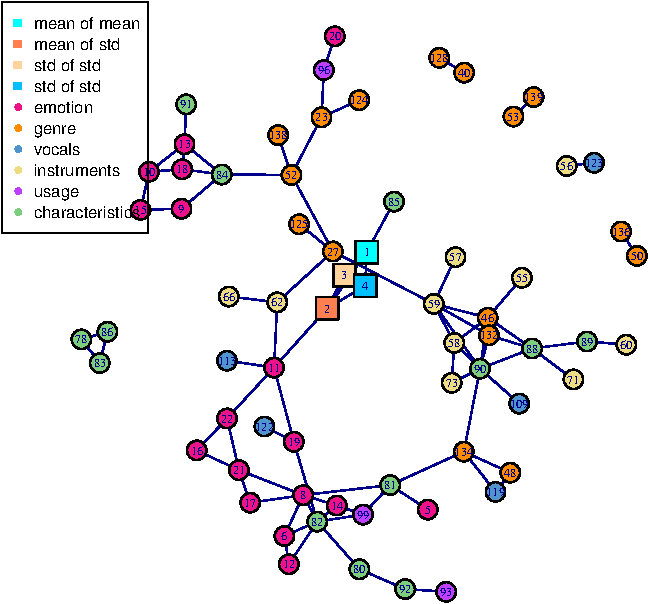
\includegraphics[width=0.49\textwidth]{./figures/real_asym2.pdf}
&
\hskip-0pt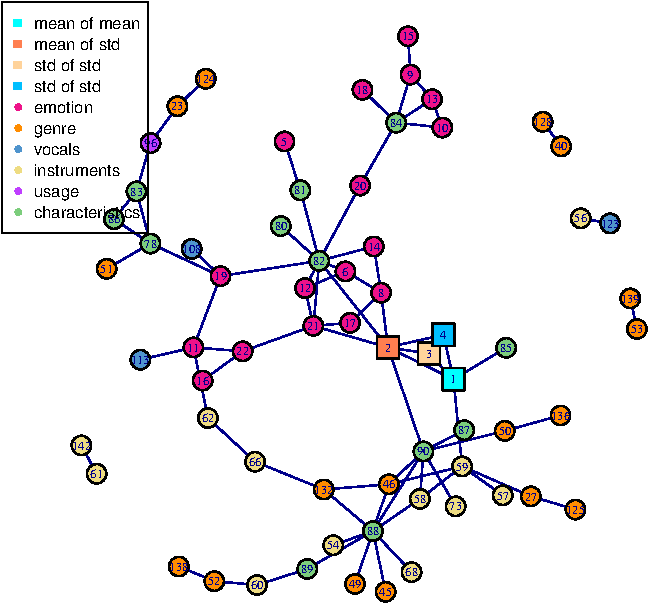
\includegraphics[width=0.49\textwidth]{./figures/real_asym.pdf}\\
\hskip-30pt (a). The asymmetric score test based on $L_k(\bbeta_k)$.&(b). Inconsistent edges of the asymmetric score test\\
\end{tabular}\\
\caption{In (a) we plot estimated graph in the \texttt{CAL500} dataset inferred by the asymmetric score test  based on the loss function $L_k(\bbeta_k)$ for testing $H_0\colon \beta_{jk}^* = 0$ for any $1\leq j < k \leq d$.  We plot the connected components of the estimated graph for illustration. Compared with Figure \ref{fig::real_data}, we observe that the two asymmetric score tests yields different graphs. In (b)  we plot the edges that appear in (a) and  Figure \ref{fig::real_data}-(a) but not in Figure \ref{fig::real_data}-(b). In other words, we plot the inconsistent edges of these two asymmetric score tests that are discovered by the pairwise score test. Thus, by taking symmetry into consideration, the pairwise score test is able to correct such inconsistency.}
\label{fig:real2}
\end{figure}


 










 









 

\vskip 0.2in
\bibliography{ref}

\end{document}
